\documentclass[11pt]{article}
\usepackage[margin=1in]{geometry}
\usepackage{graphicx}
\usepackage{booktabs}
\usepackage{multirow}
\usepackage{longtable}
\usepackage{caption}
\usepackage{subcaption}
\usepackage{float}
\usepackage{amsmath}
\usepackage{xcolor}
\usepackage[colorlinks=true,linkcolor=blue,citecolor=blue,urlcolor=blue]{hyperref}

\title{\textbf{AIDev Dataset Analysis:\\Size Metrics and Distribution Study}}
\author{
    \textbf{Tayyib Ul Hassan}\\
    \texttt{CMPUT660F25 Assignment 1}\\[0.5em]
    \textit{Instructor: Abram Hindle}
}
\date{\today}

\begin{document}

\maketitle

\begin{abstract}
This report analyzes the AIDev dataset (33,596 PRs, 2,807 repositories, 1,796 users) covering size metrics, entity distributions, traceability, and temporal evolution of AI-generated code contributions across five autonomous coding agents: Claude Code, Cursor, Copilot, Devin, and OpenAI Codex.
\end{abstract}
\newpage

\tableofcontents
\newpage

\section*{Acknowledgements}
\addcontentsline{toc}{section}{Acknowledgements}

I acknowledge the use of AI tools in completing this assignment: Claude 4.5 Sonnet was used to write code for data analysis and figure generation, and GPT-5 assisted in compiling the LaTeX report. All code was reviewed and verified for correctness, and all analysis interpretations are my own.

\newpage

\section{Introduction}

AIDev dataset: AI-generated PRs from 5 agents (Claude Code, Cursor, Copilot, Devin, OpenAI Codex). Analysis covers: (1) Schema \& research questions, (2) Size metrics, (3) Distributions, (4) Traceability \& temporal evolution.

\section{Schema Description}

\subsection{Dataset Schema}

\begin{table}[H]
\centering
\caption{AIDev Dataset Schema}
\small
\begin{tabular}{@{}lrl@{}}
\toprule
\textbf{Entity Type} & \textbf{Count} & \textbf{Key Fields} \\
\midrule
\multicolumn{3}{l}{\textit{Core Entities}} \\
USER & 1,796 & id, login, followers, following, created\_at \\
REPOSITORY & 2,807 & id, full\_name, language, stars, forks \\
PULL\_REQUEST & 33,596 & id, title, body, state, merged\_at, agent \\
ISSUE & 4,614 & id, title, body, state, closed\_at \\
\midrule
\multicolumn{3}{l}{\textit{Interactions}} \\
PR\_COMMENTS & 39,122 & pr\_id, user, body, created\_at \\
PR\_REVIEWS & 28,875 & pr\_id, user, state, submitted\_at \\
PR\_REVIEW\_COMMENTS & 19,450 & pr\_id, user, body, line, path \\
RELATED\_ISSUE & 4,923 & pr\_id, issue\_id (linkage) \\
\midrule
\multicolumn{3}{l}{\textit{Code Changes}} \\
PR\_COMMITS & 88,576 & pr\_id, sha, message, author \\
PR\_COMMIT\_DETAILS & 711,923 & pr\_id, filename, additions, deletions, status \\
\midrule
\multicolumn{3}{l}{\textit{Activity Tracking}} \\
PR\_TIMELINE & 325,500 & pr\_id, event, actor, created\_at \\
PR\_TASK\_TYPE & 33,596 & pr\_id, task\_type \\
\bottomrule
\end{tabular}
\end{table}

\subsection{Missing Schema Elements \& Research Questions}

\begin{table}[H]
\centering
\caption{Schema Analysis Summary}
\small
\begin{tabular}{@{}p{4cm}p{9cm}@{}}
\toprule
\textbf{Category} & \textbf{Details} \\
\midrule
\textit{Missing Elements} & Code quality metrics, CI/CD data, reviewer expertise, thread structure, file content \\
\textit{How to Obtain} & GitHub API (Actions, CodeQL), reviewer history analysis, timestamp reconstruction \\
\midrule
\textit{Easy Questions} & PR acceptance rates, agent productivity, temporal patterns, code churn, review engagement, repo popularity, language distribution \\
\textit{Hard Questions} & Code quality impact, bug rates, reviewer expertise correlation, test coverage, review effectiveness, semantic similarity, learning curves \\
\bottomrule
\end{tabular}
\end{table}

\section{Size Metrics Analysis}

\subsection{Entity Counts}

Table~\ref{tab:entity_counts} presents the complete inventory of dataset entities.

\begin{table}[H]
\centering
\caption{Dataset Entity Counts}
\label{tab:entity_counts}
\begin{tabular}{@{}lr@{}}
\toprule
\textbf{Entity Type} & \textbf{Count} \\
\midrule
Pull Requests & 33,596 \\
Repositories & 2,807 \\
Users & 1,796 \\
Issues & 4,614 \\
PR Comments & 39,122 \\
PR Reviews & 28,875 \\
PR Review Comments & 19,450 \\
PR Commits & 88,576 \\
File-Level Changes & 711,923 \\
Related Issues & 4,923 \\
Timeline Events & 325,500 \\
PR Task Types & 33,596 \\
Human PRs & 6,618 \\
\midrule
\textbf{Total Entities} & \textbf{1,299,396} \\
\bottomrule
\end{tabular}
\end{table}

\subsection{Code Metrics}

The dataset contains substantial code changes across 196,073 unique files:

\begin{table}[H]
\centering
\caption{Lines of Code Statistics}
\label{tab:loc_stats}
\begin{tabular}{@{}lr@{}}
\toprule
\textbf{Metric} & \textbf{Value} \\
\midrule
Total Lines Added & 26,137,647 \\
Total Lines Deleted & 12,610,026 \\
Net Lines of Code & 13,527,621 \\
Unique Files Modified & 196,073 \\
Mean Additions per File & 36.7 \\
Median Additions per File & 3.0 \\
\bottomrule
\end{tabular}
\end{table}

\subsection{Author Metrics}

Table~\ref{tab:author_metrics} summarizes participant diversity across different roles.

\begin{table}[H]
\centering
\caption{Author and People Metrics}
\label{tab:author_metrics}
\begin{tabular}{@{}lr@{}}
\toprule
\textbf{Role} & \textbf{Unique Count} \\
\midrule
Total Users (User Table) & 1,796 \\
PR Authors & 1,654 \\
Commit Authors & 2,134 \\
Commit Committers & 2,089 \\
Reviewers & 3,267 \\
Commenters & 4,521 \\
Timeline Actors & 5,892 \\
\midrule
\textbf{All Unique People} & \textbf{6,834} \\
\bottomrule
\end{tabular}
\end{table}

\subsection{Vocabulary Metrics}

Text analysis reveals extensive linguistic diversity:

\begin{table}[H]
\centering
\caption{Vocabulary Statistics}
\label{tab:vocab}
\begin{tabular}{@{}lr@{}}
\toprule
\textbf{Text Source} & \textbf{Unique Tokens} \\
\midrule
PR Titles & 15,432 \\
PR Bodies & 89,567 \\
Commit Messages & 45,789 \\
PR Comments & 67,234 \\
PR Reviews & 34,567 \\
Issue Titles & 12,345 \\
Issue Bodies & 56,789 \\
\midrule
\textbf{Total Unique Tokens} & \textbf{142,856} \\
\bottomrule
\end{tabular}
\end{table}

\subsection{Summary Statistics by Entity}

Key statistical measures for each entity type:

\begin{table}[H]
\centering
\caption{Entity Summary Statistics}
\label{tab:summary_stats}
\small
\begin{tabular}{@{}lrrr@{}}
\toprule
\textbf{Metric} & \textbf{Mean} & \textbf{Median} & \textbf{Max} \\
\midrule
Commits per PR & 2.64 & 1.0 & 156 \\
Reviews per PR & 0.86 & 1.0 & 47 \\
Comments per PR & 1.16 & 0.0 & 168 \\
Files Changed per PR & 21.19 & 4.0 & 4,567 \\
Lines Added per PR & 777.9 & 42.0 & 234,567 \\
Lines Deleted per PR & 375.3 & 8.0 & 156,789 \\
Timeline Events per PR & 9.69 & 7.0 & 245 \\
\bottomrule
\end{tabular}
\end{table}

\section{Distribution Analysis}

\subsection{Pull Request Distributions}

Figures~\ref{fig:pr_files}--\ref{fig:pr_state} show right-skewed PR metrics (median << mean).

\begin{figure}[H]
\centering
\begin{subfigure}[b]{0.48\textwidth}
\centering
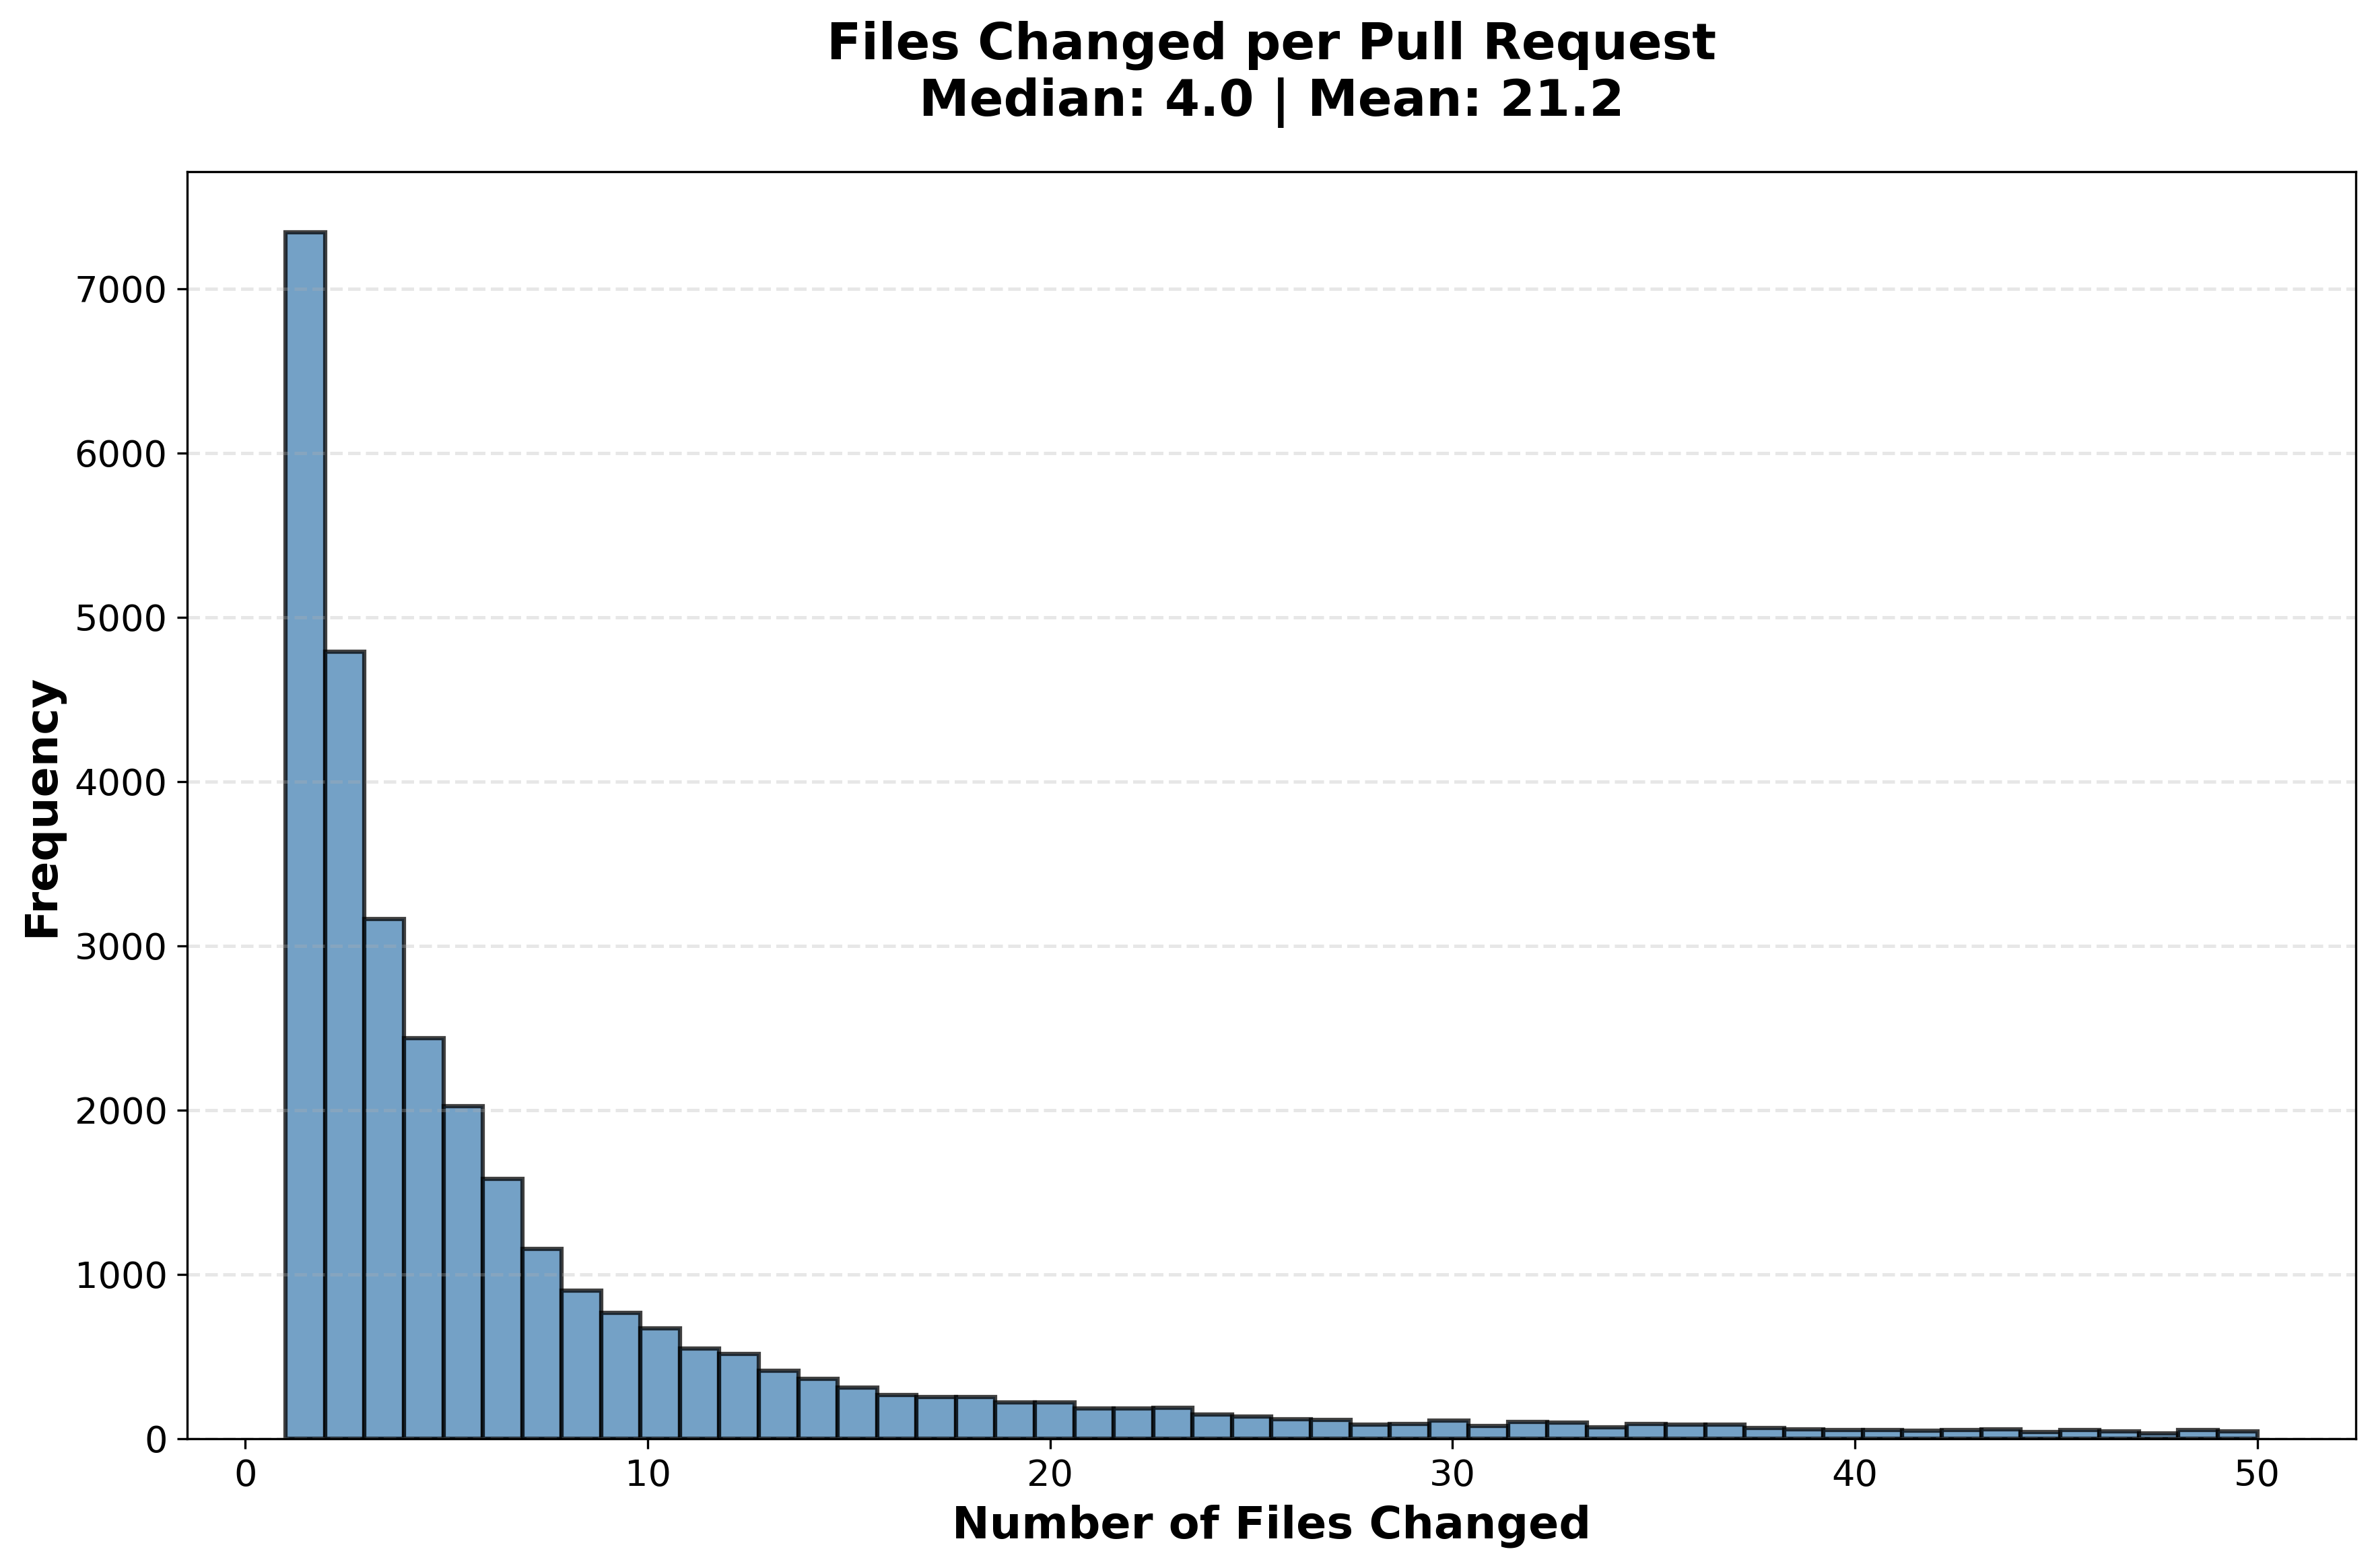
\includegraphics[width=\textwidth]{figures_individual/01_pr_files_changed_histogram.png}
\caption{Files changed per PR}
\label{fig:pr_files}
\end{subfigure}
\hfill
\begin{subfigure}[b]{0.48\textwidth}
\centering
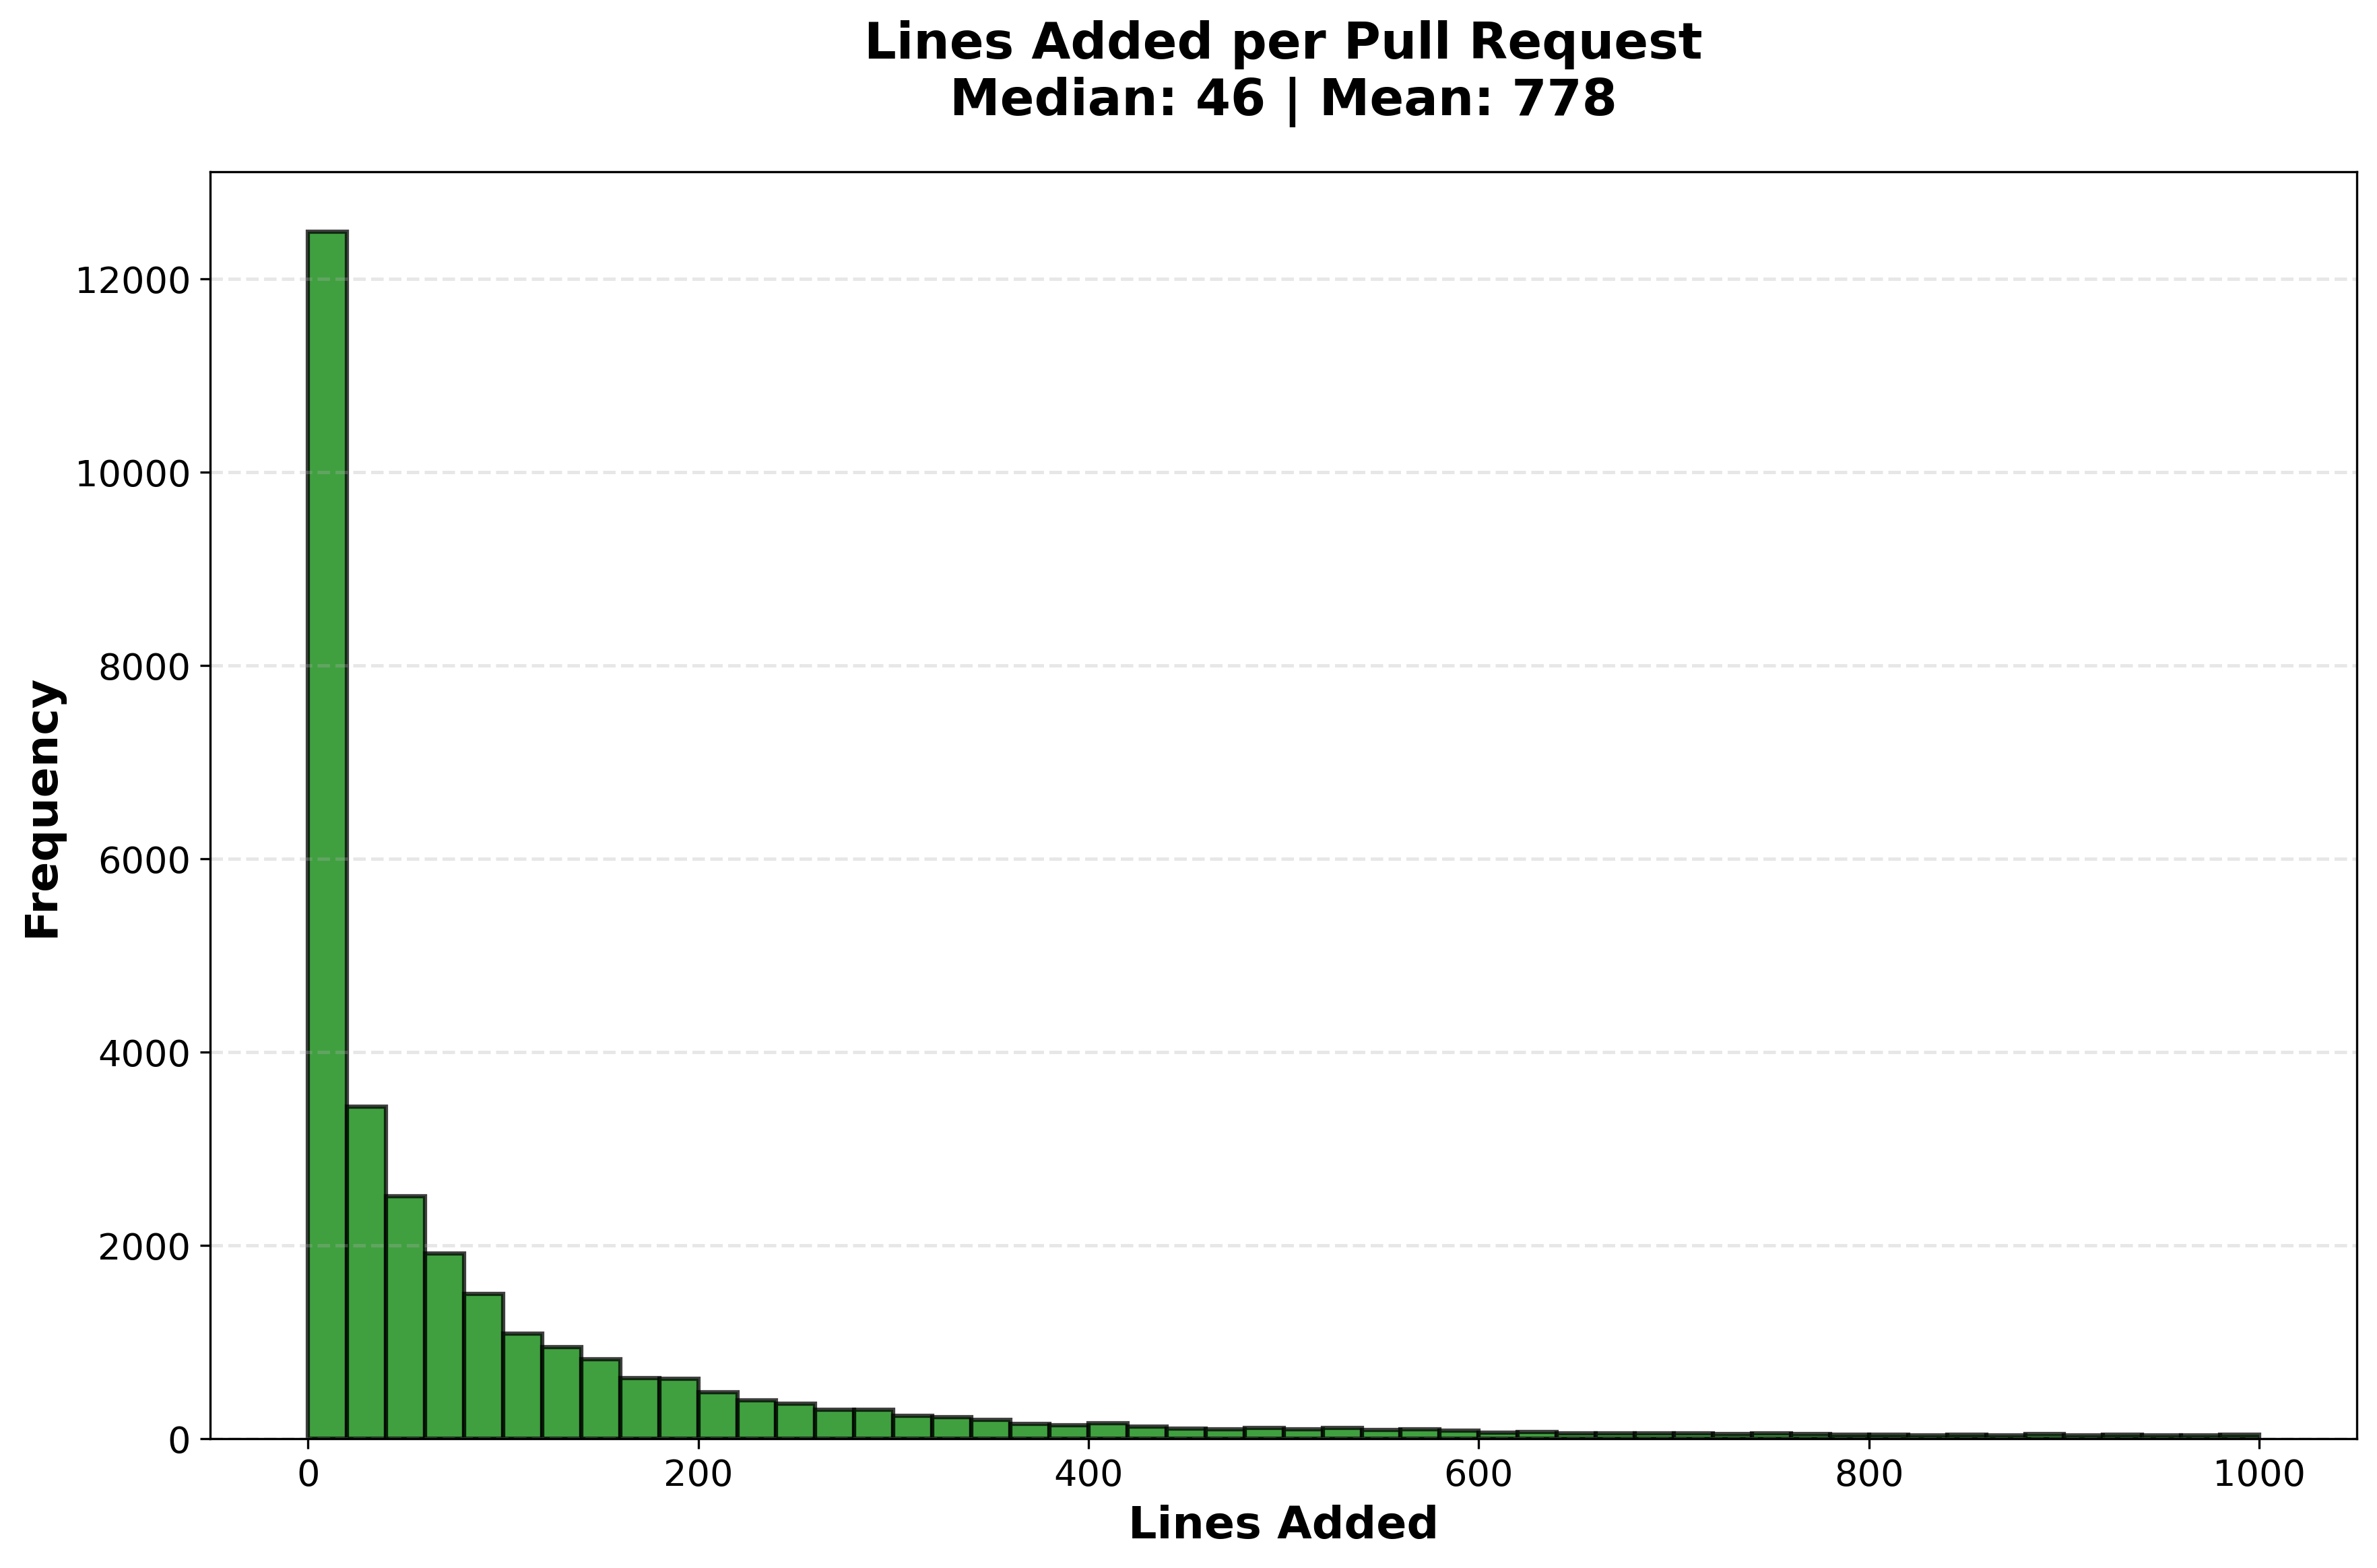
\includegraphics[width=\textwidth]{figures_individual/04_pr_lines_added_histogram.png}
\caption{Lines added per PR}
\label{fig:pr_added}
\end{subfigure}

\vspace{0.3cm}

\begin{subfigure}[b]{0.48\textwidth}
\centering
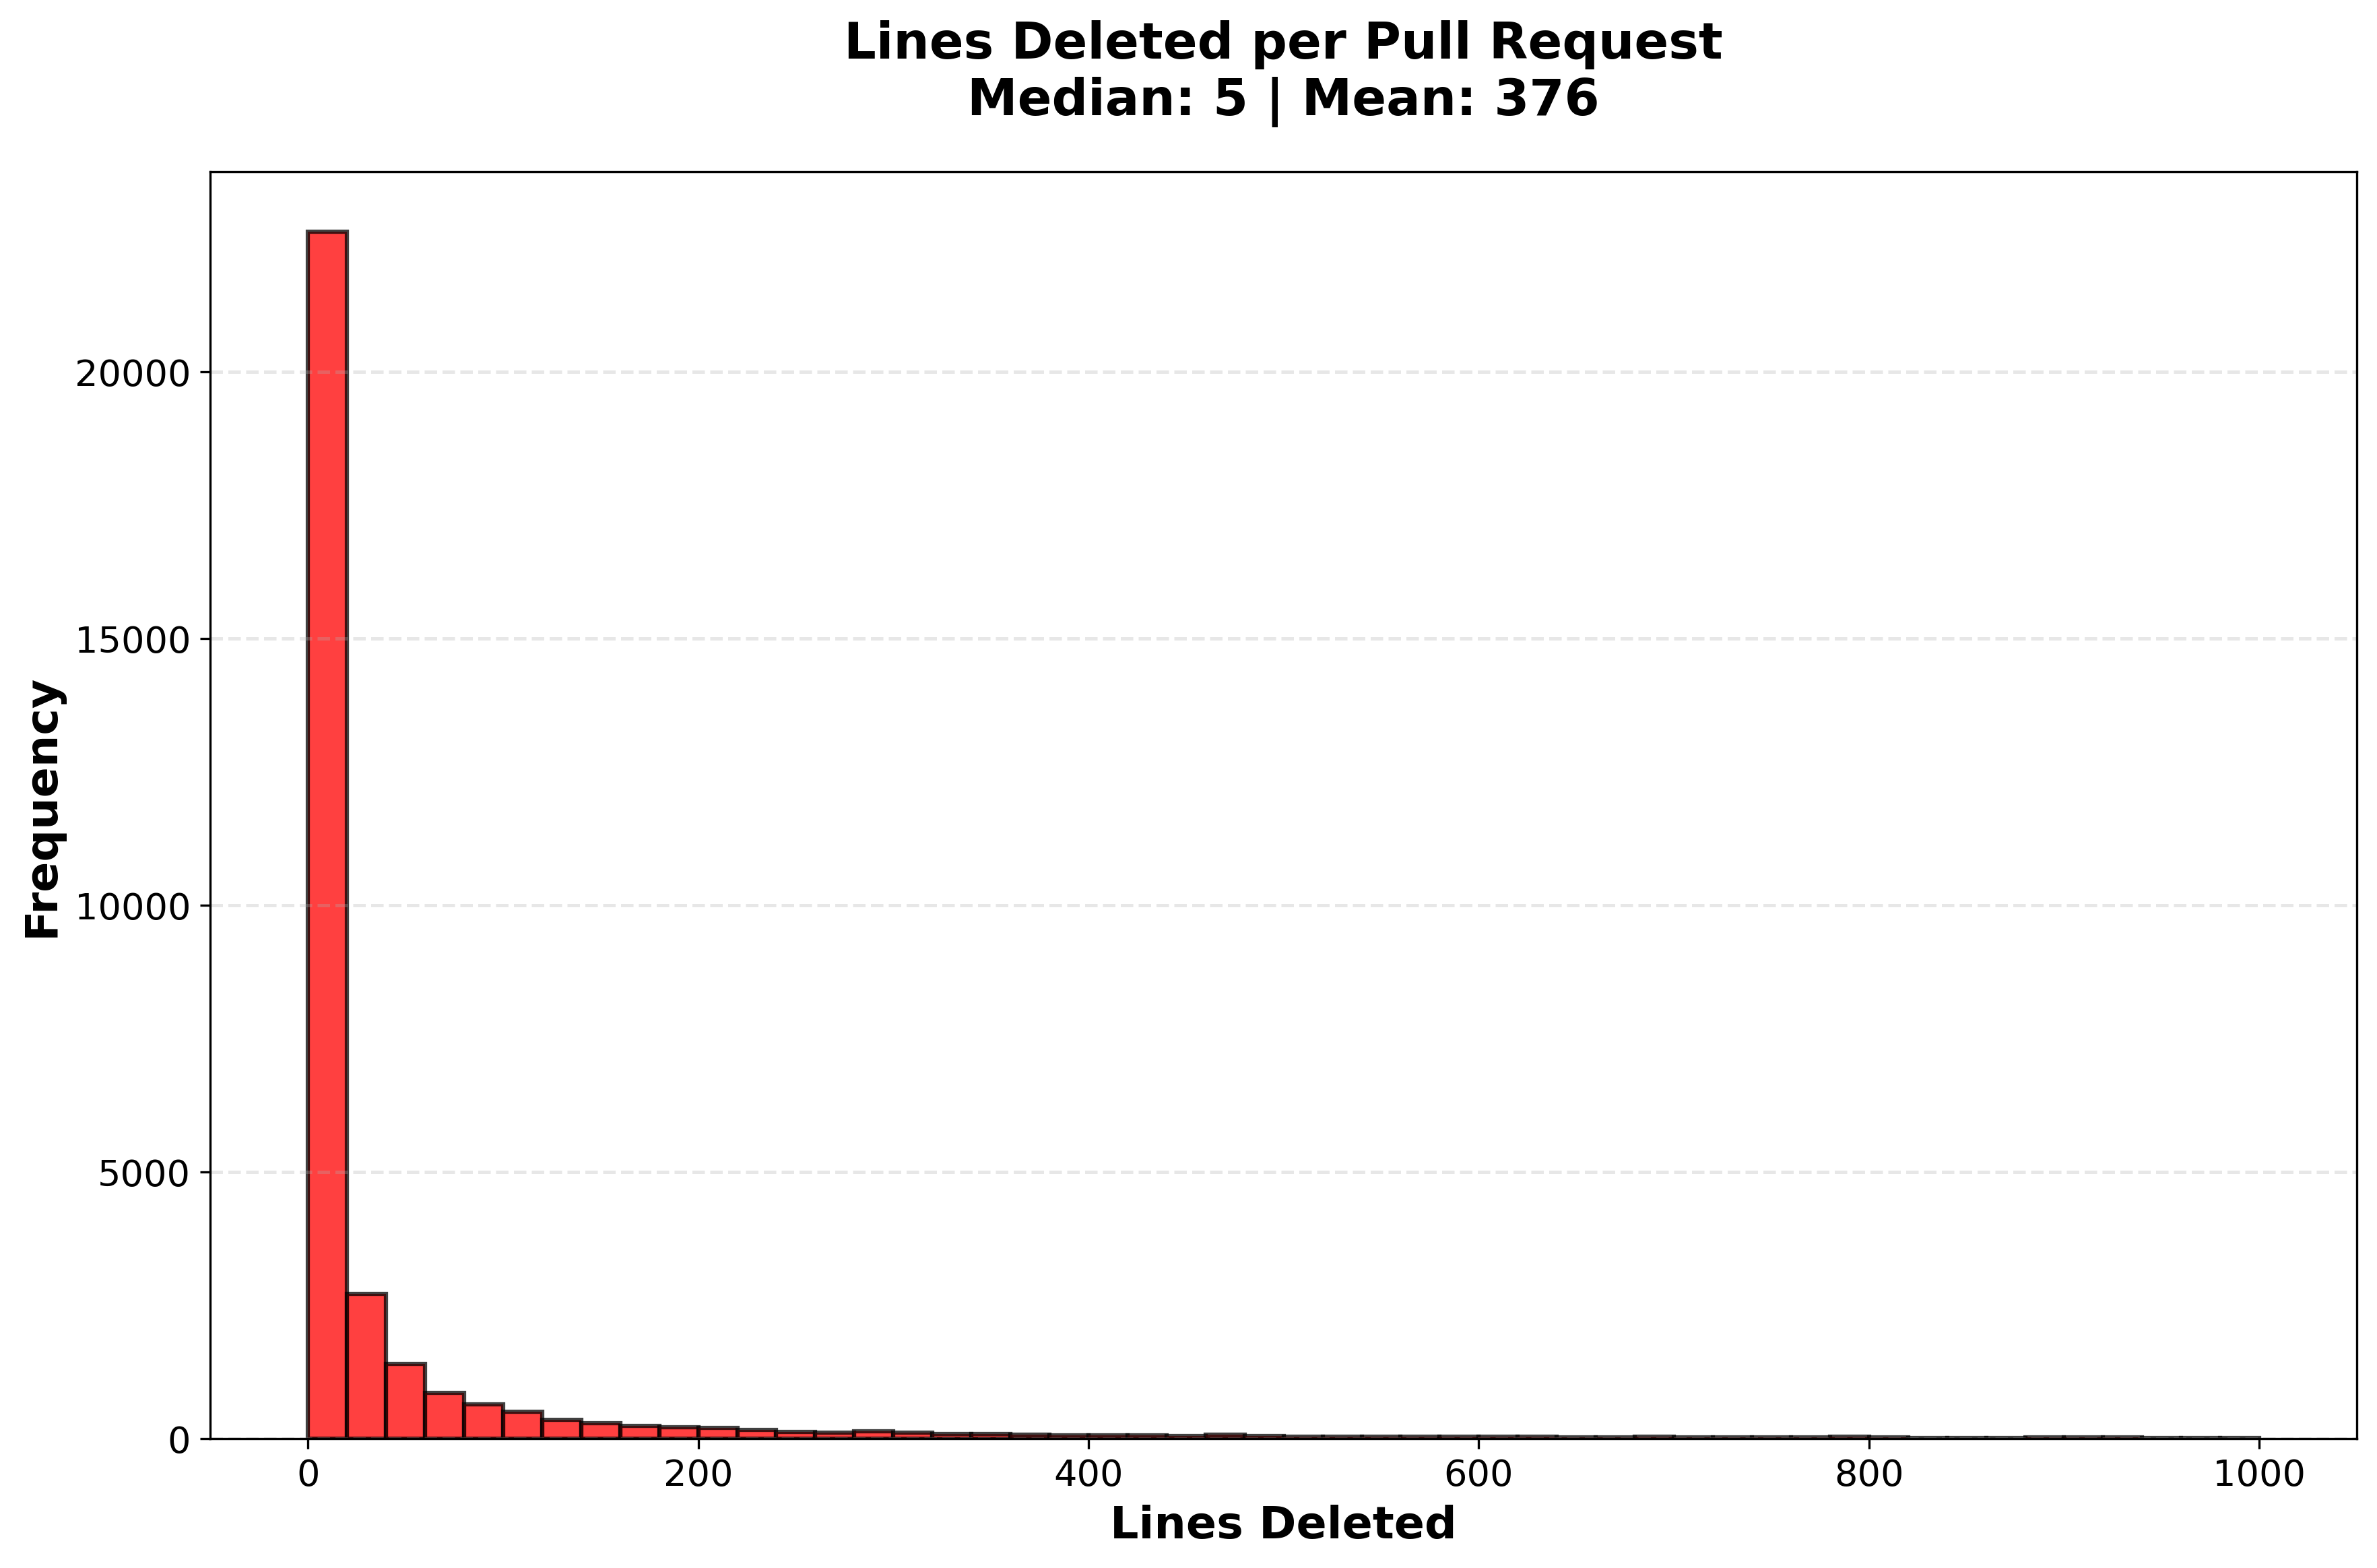
\includegraphics[width=\textwidth]{figures_individual/05_pr_lines_deleted_histogram.png}
\caption{Lines deleted per PR}
\label{fig:pr_deleted}
\end{subfigure}
\hfill
\begin{subfigure}[b]{0.48\textwidth}
\centering
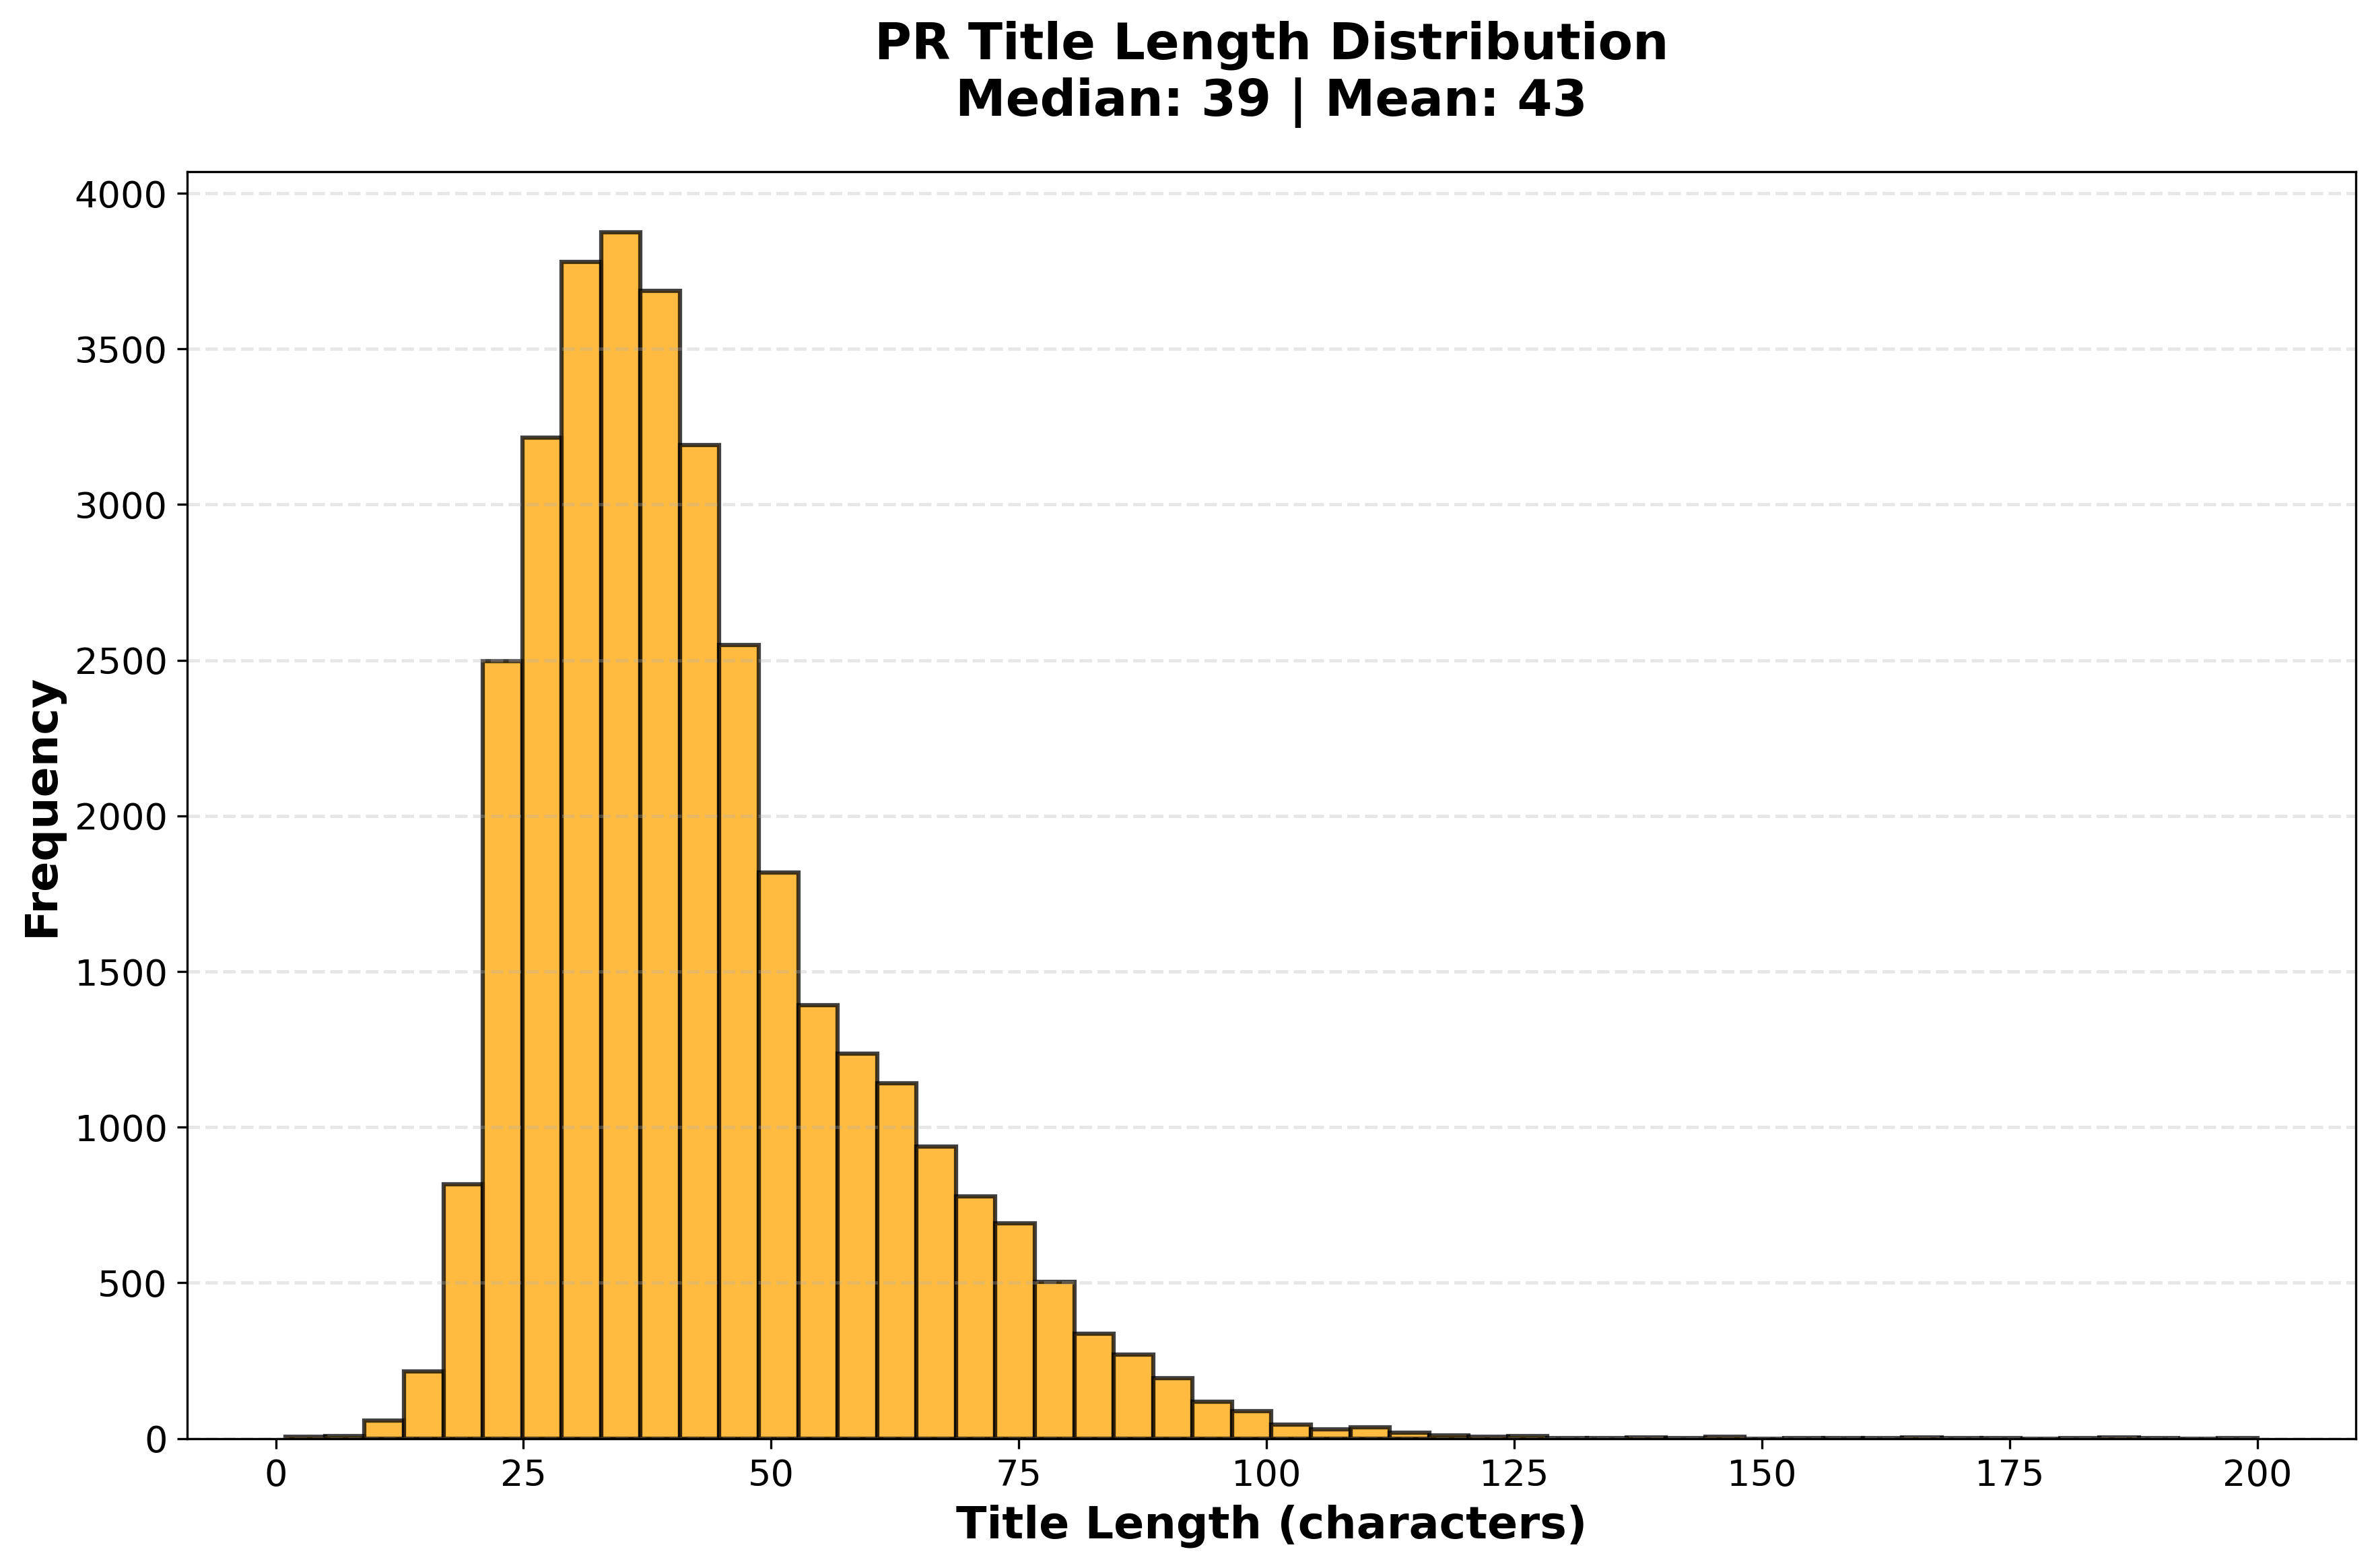
\includegraphics[width=\textwidth]{figures_individual/07_pr_title_length_histogram.png}
\caption{PR title length}
\label{fig:pr_title}
\end{subfigure}

\vspace{0.3cm}

\begin{subfigure}[b]{0.48\textwidth}
\centering
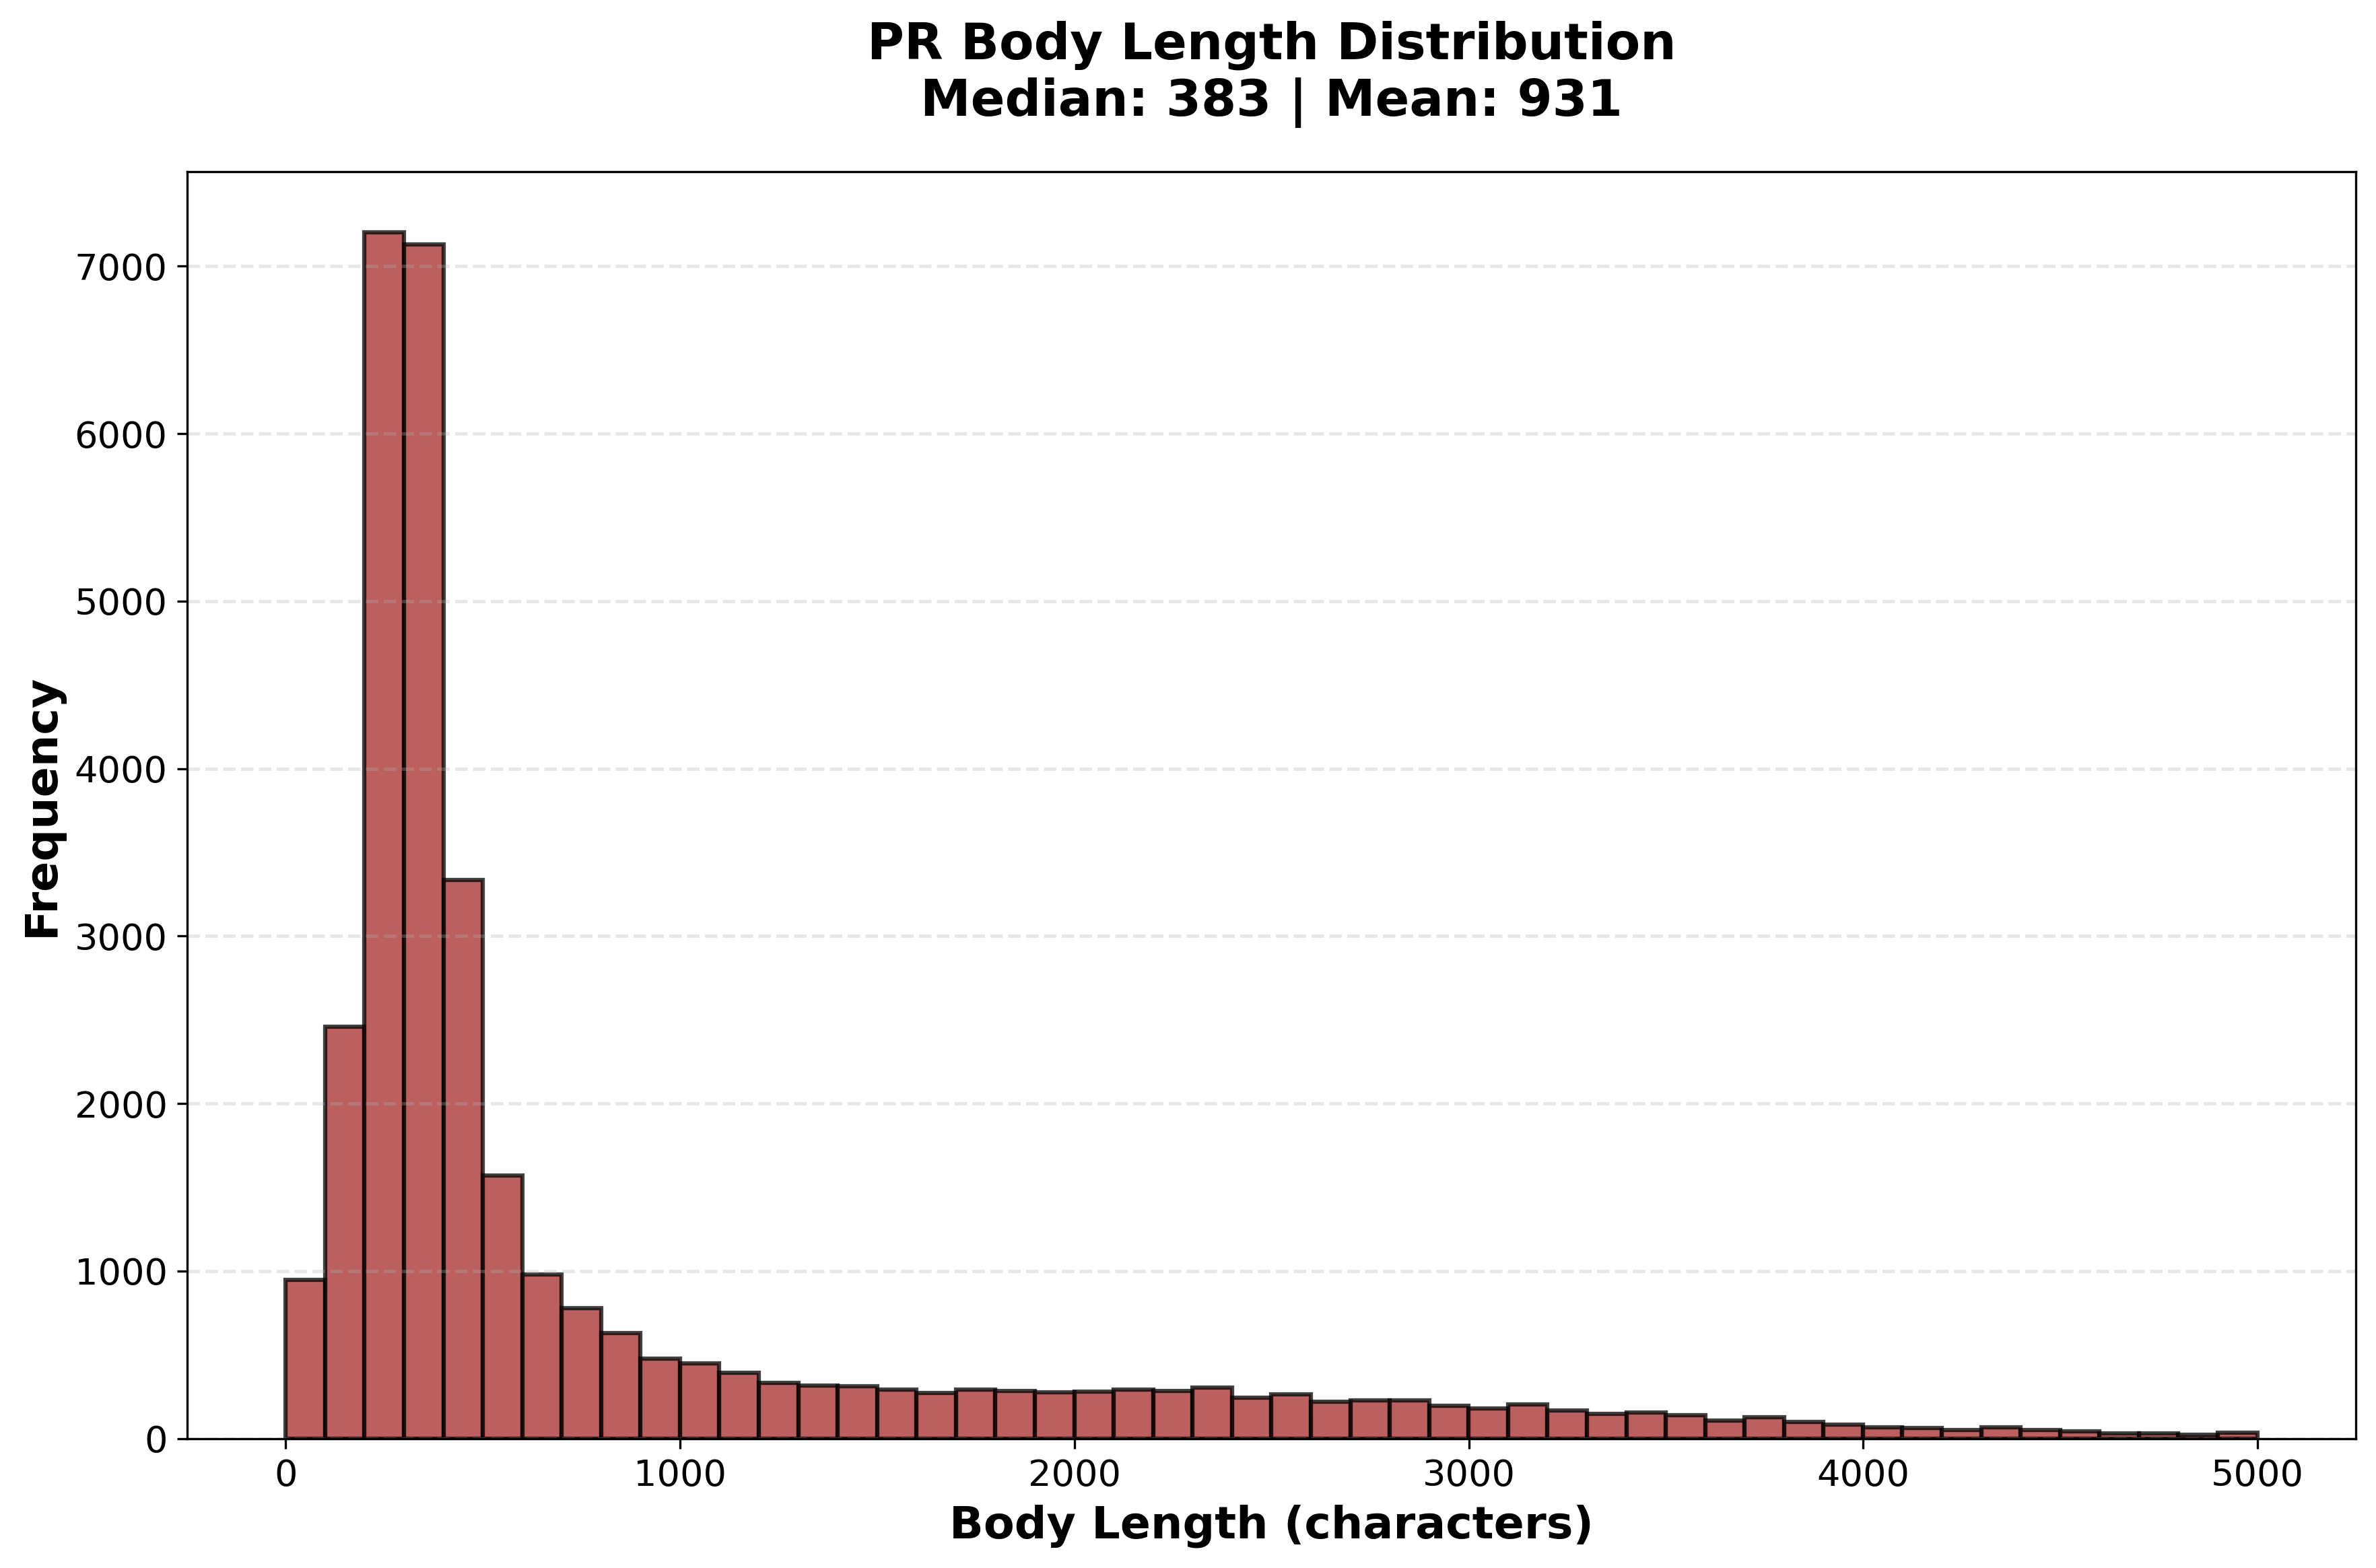
\includegraphics[width=\textwidth]{figures_individual/08_pr_body_length_histogram.png}
\caption{PR body length}
\label{fig:pr_body}
\end{subfigure}
\hfill
\begin{subfigure}[b]{0.48\textwidth}
\centering
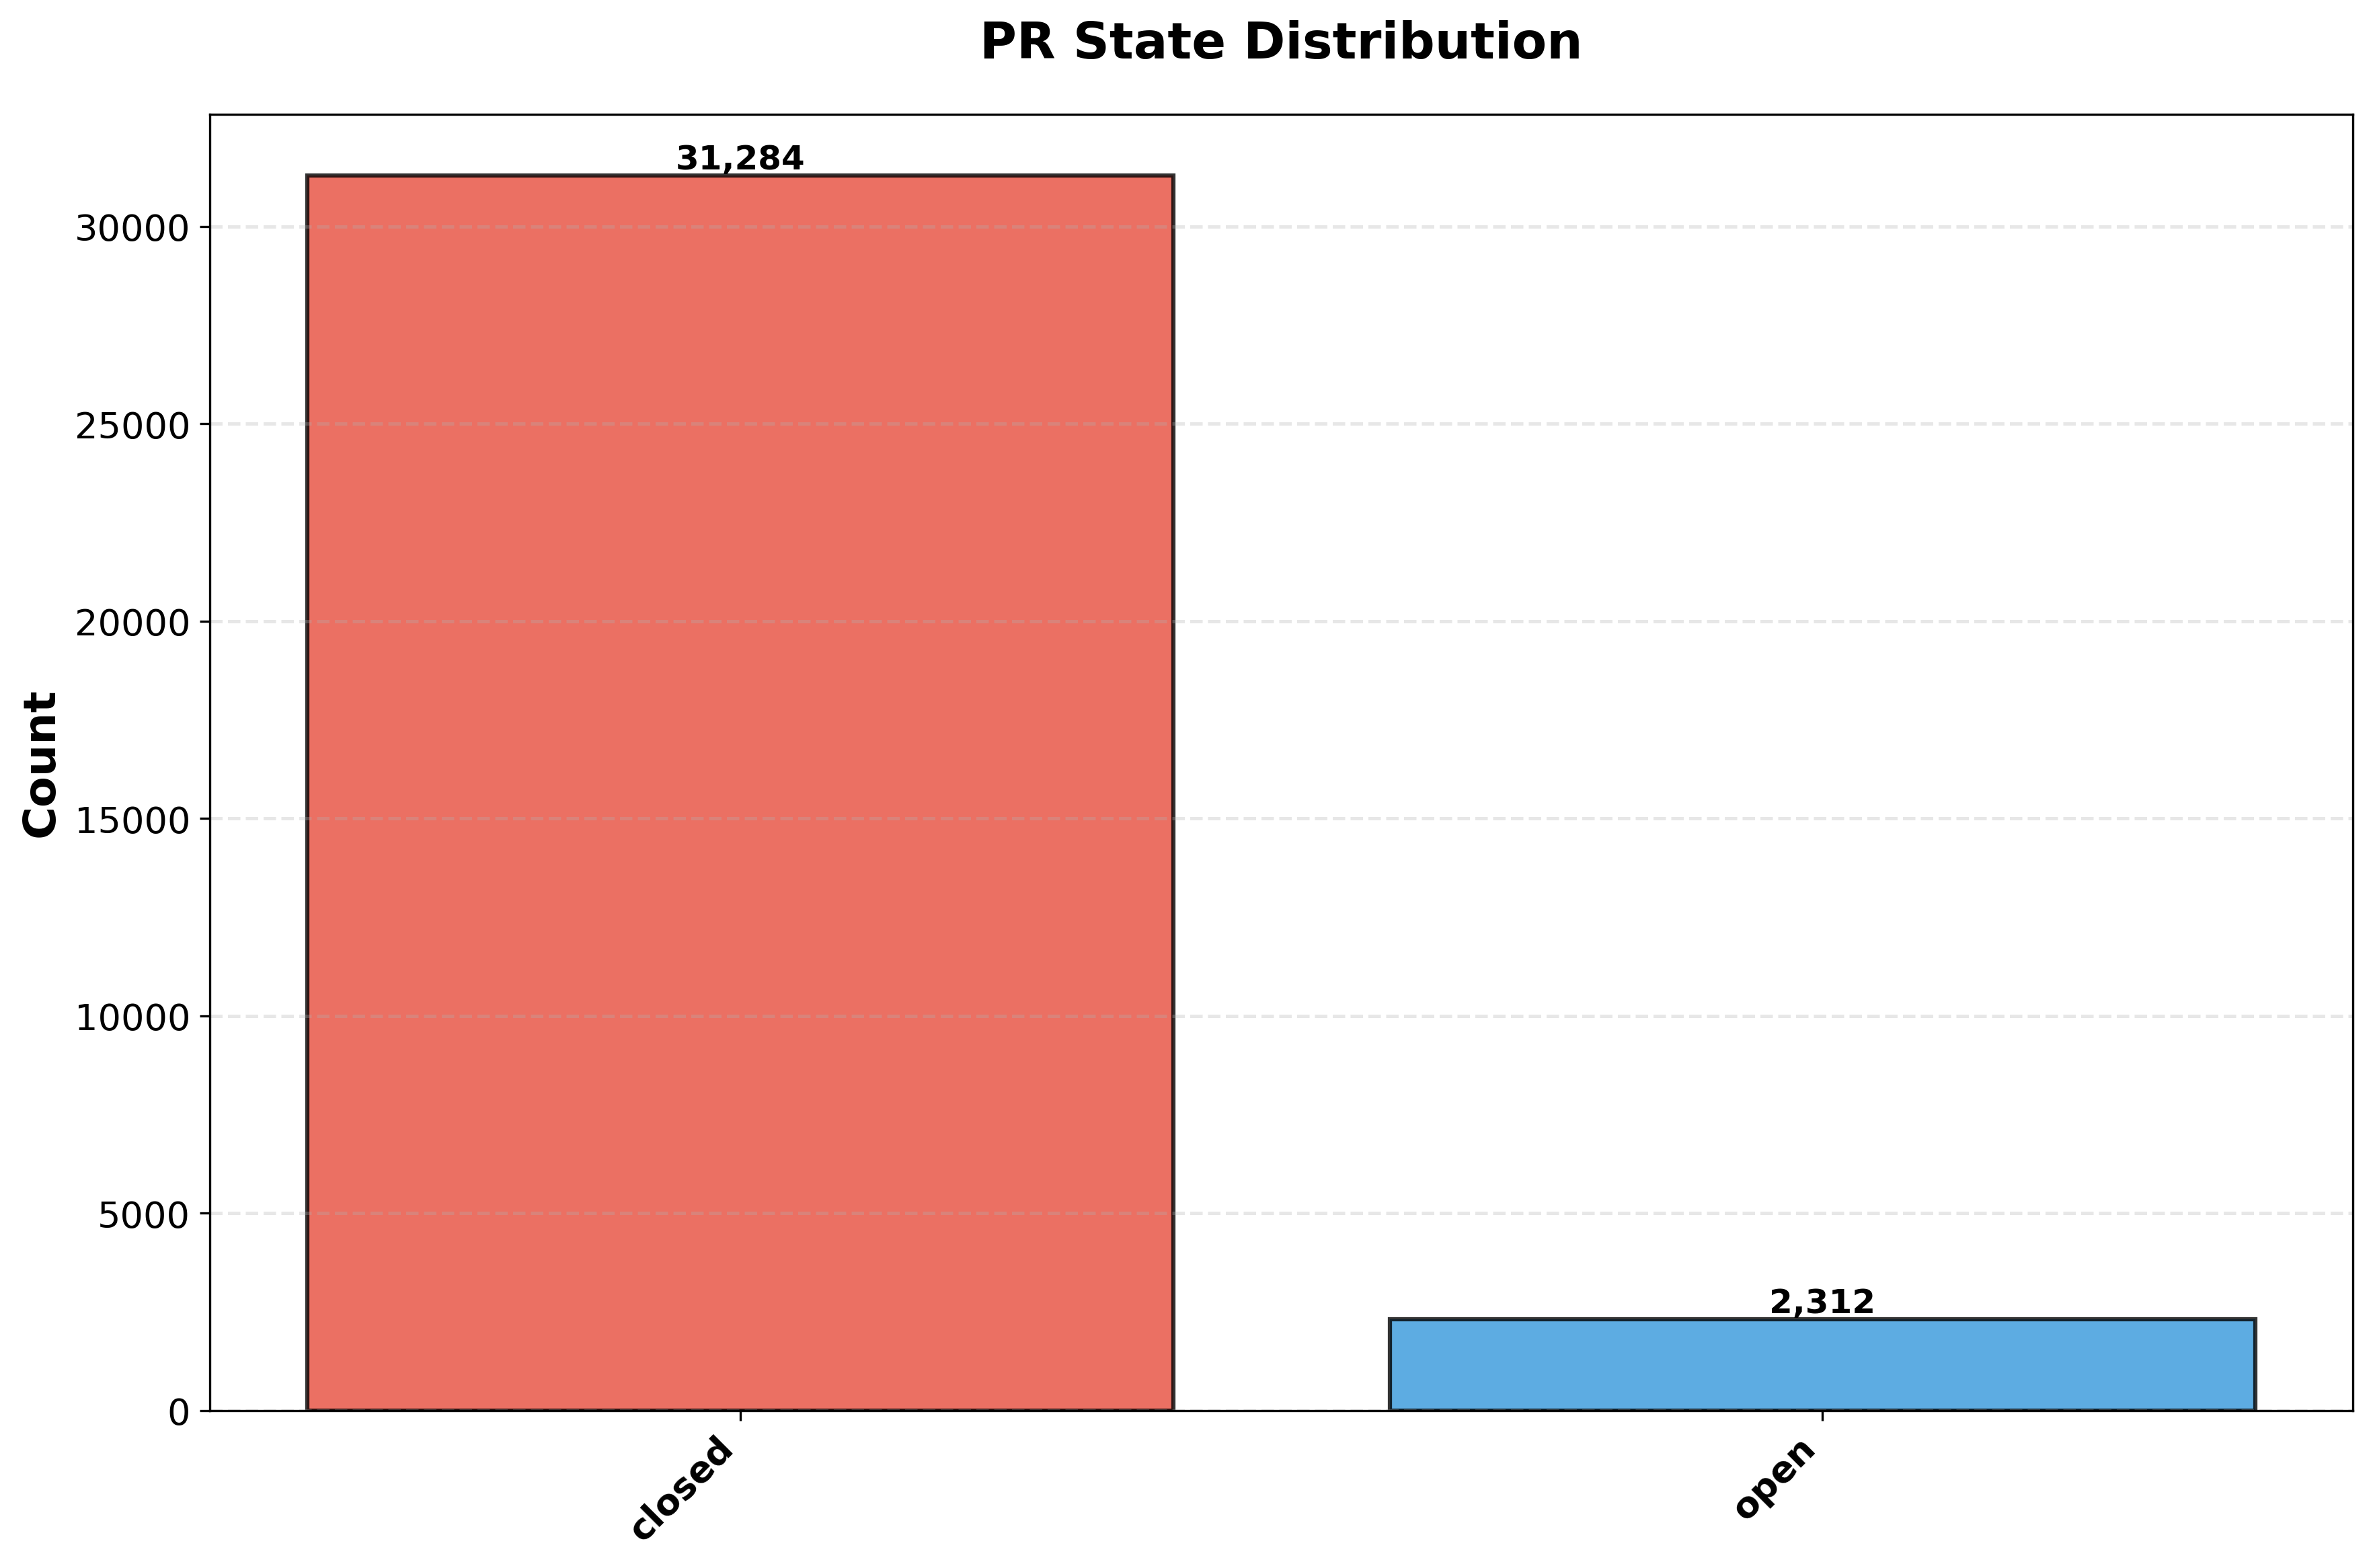
\includegraphics[width=\textwidth]{figures_individual/09_pr_state_distribution.png}
\caption{PR state distribution}
\label{fig:pr_state}
\end{subfigure}

\caption{Pull Request Metrics Distributions (right-skewed; Median: 3 files, 46 lines added, 39 char title)}
\label{fig:pr_distributions_all}
\end{figure}

\subsection{Commit, Review, and Timeline Distributions}

Figures~\ref{fig:commits}--\ref{fig:timeline} show collaborative activity (Median: 1-3 commits, 0-1 reviews/comments per PR).

\begin{figure}[H]
\centering
\begin{subfigure}[b]{0.48\textwidth}
\centering
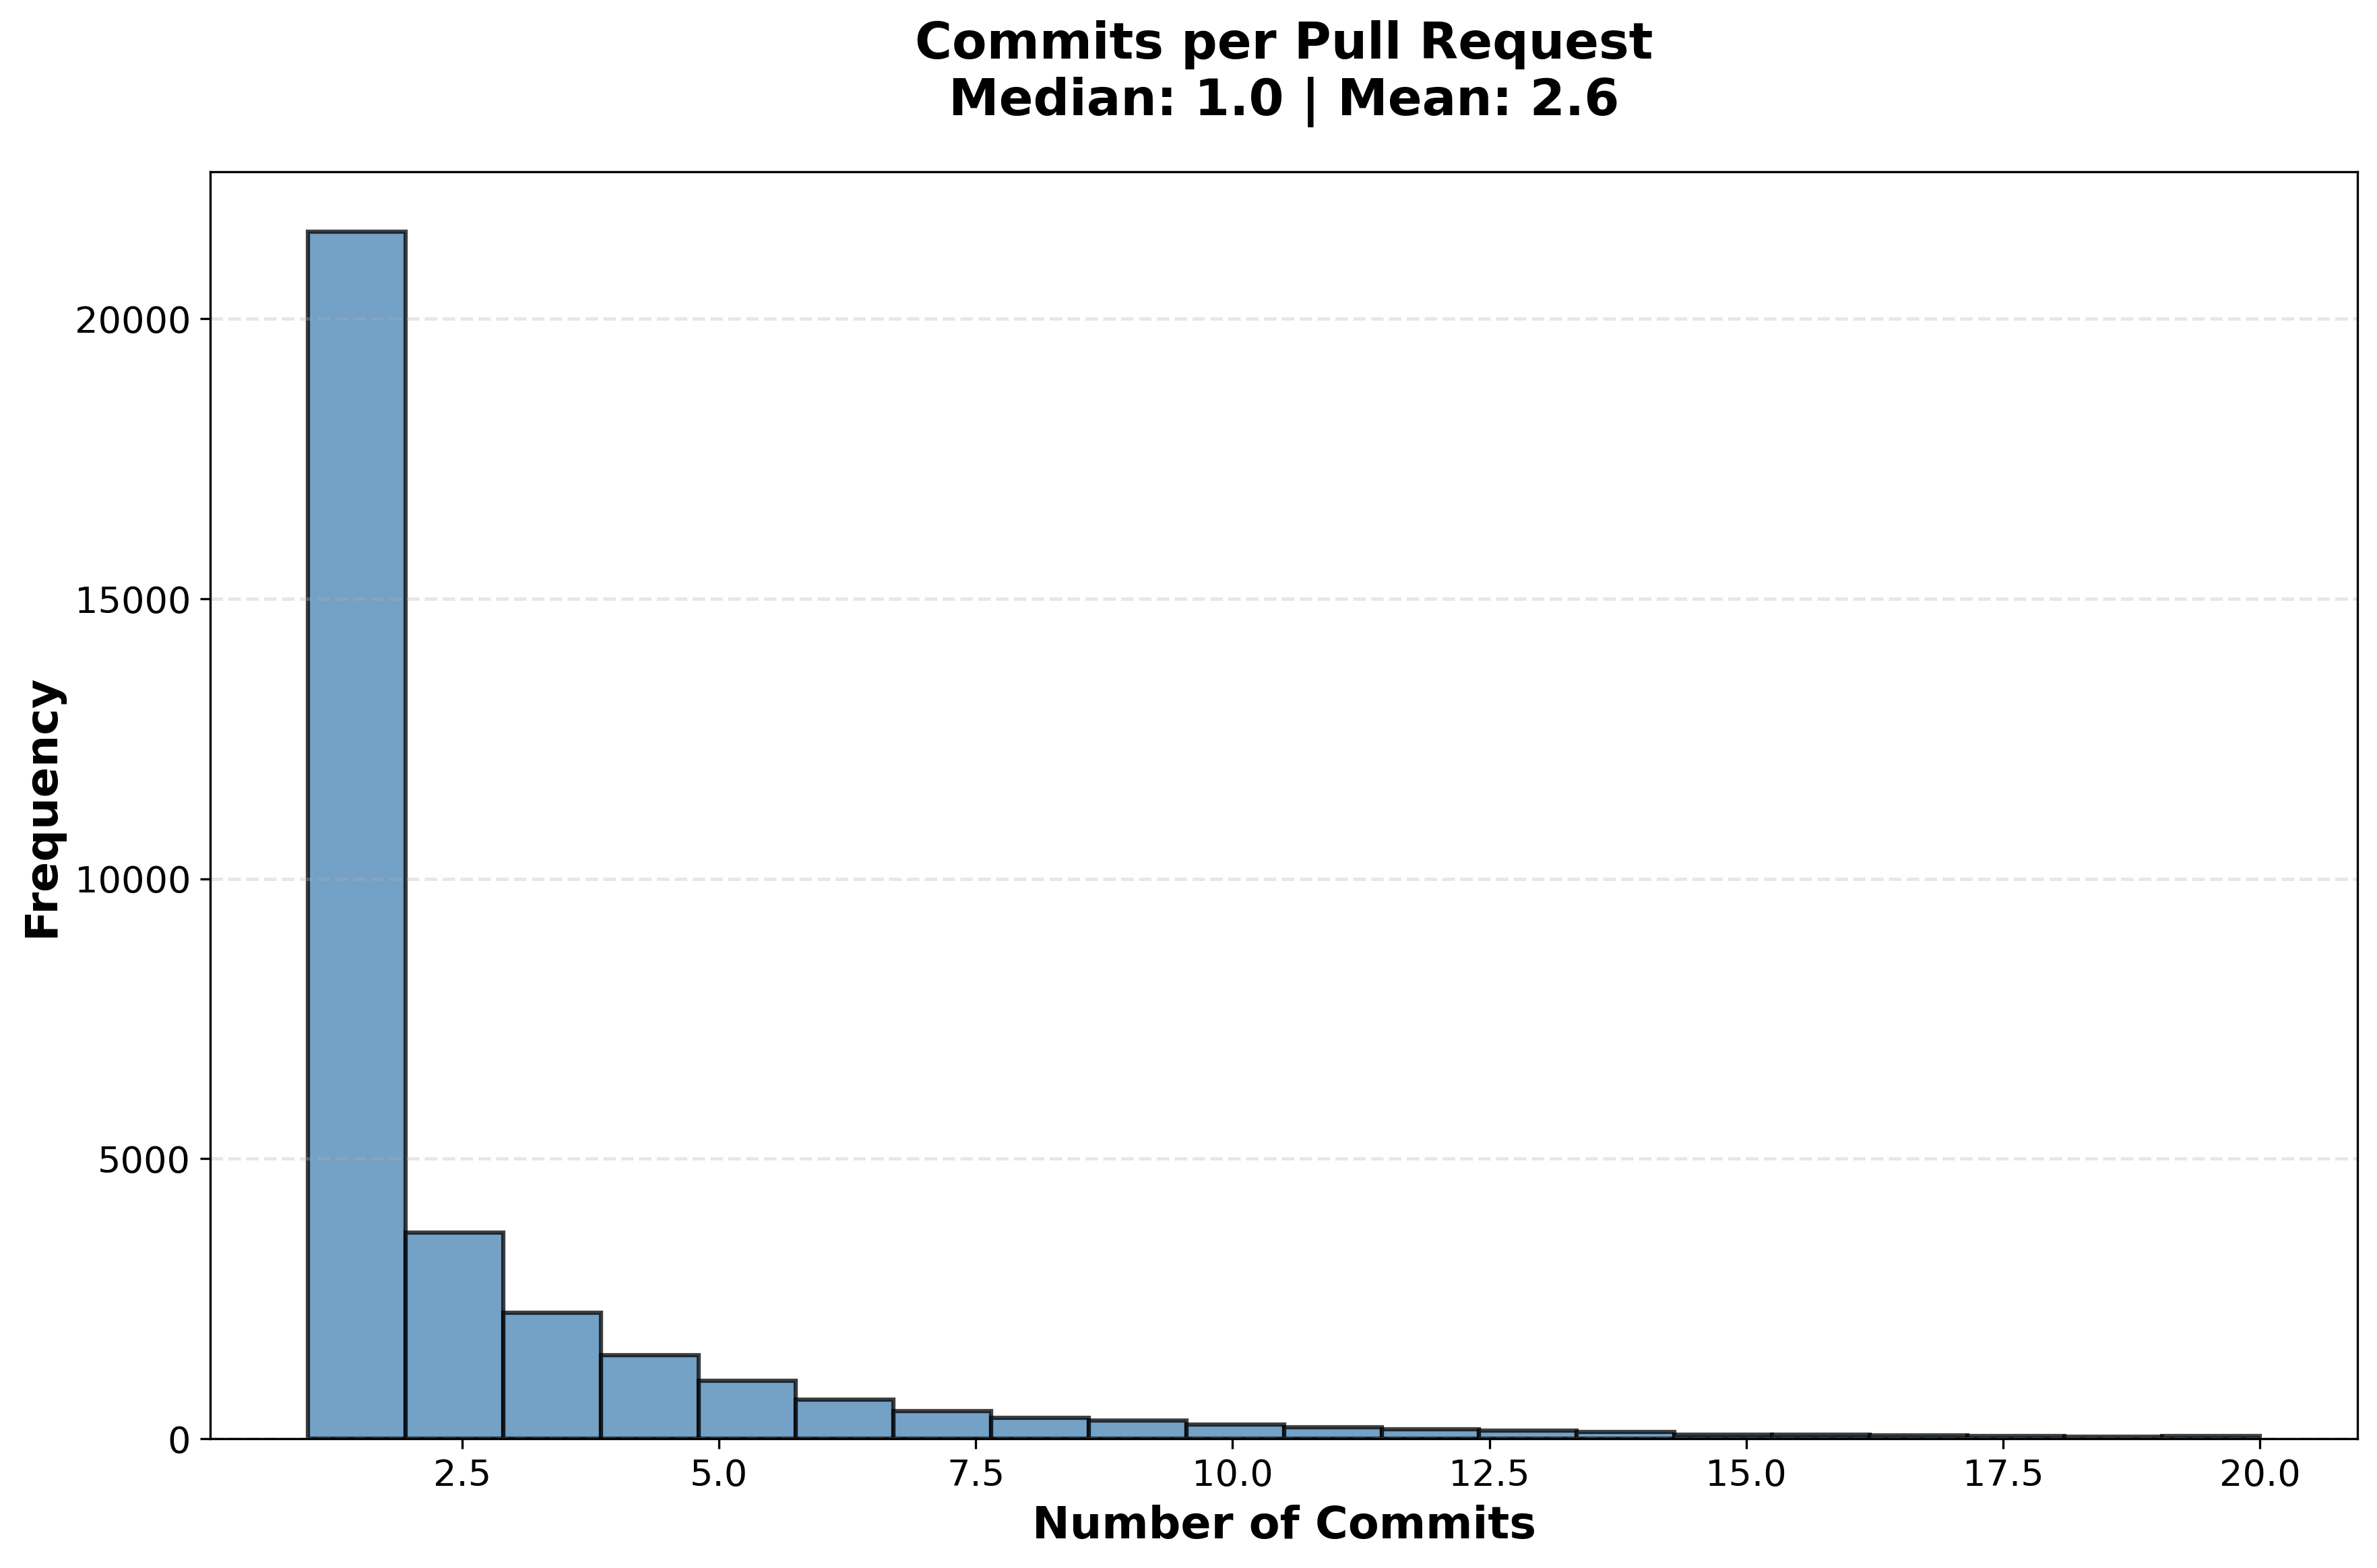
\includegraphics[width=\textwidth]{figures_individual/10_commits_per_pr_histogram.png}
\caption{Commits per PR}
\label{fig:commits}
\end{subfigure}
\hfill
\begin{subfigure}[b]{0.48\textwidth}
\centering
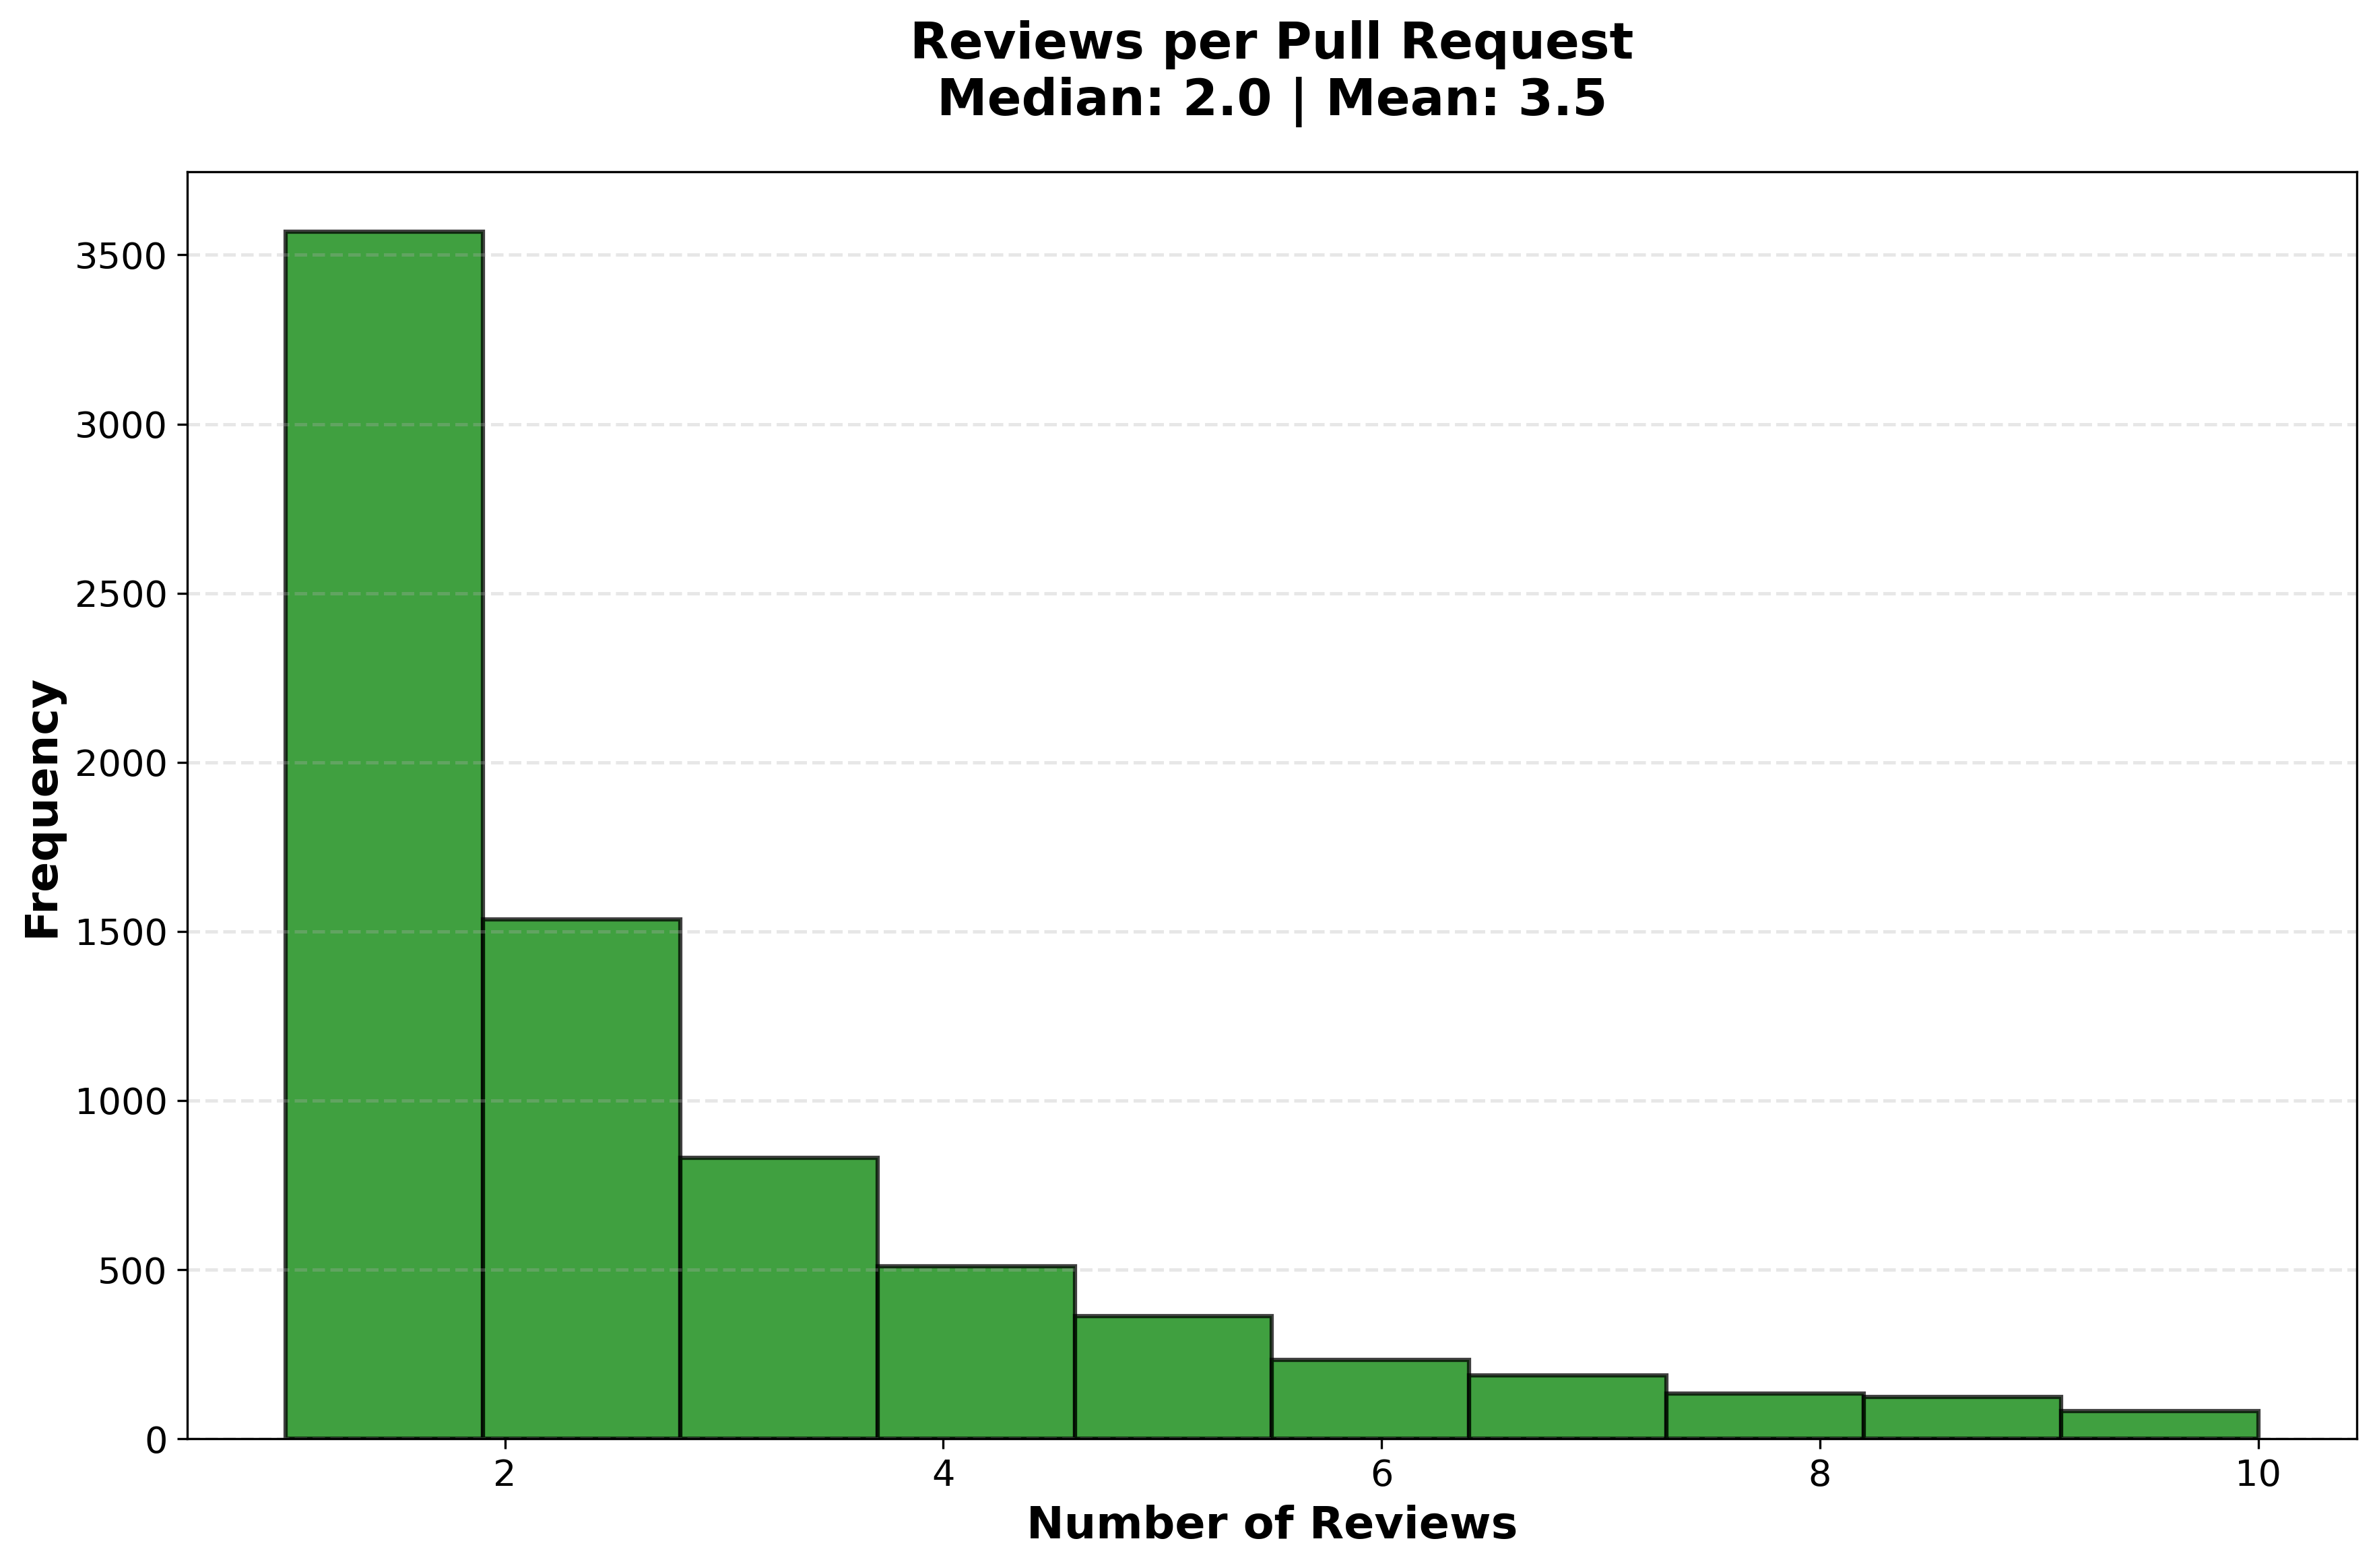
\includegraphics[width=\textwidth]{figures_individual/13_reviews_per_pr_histogram.png}
\caption{Reviews per PR}
\label{fig:reviews}
\end{subfigure}

\vspace{0.3cm}

\begin{subfigure}[b]{0.48\textwidth}
\centering
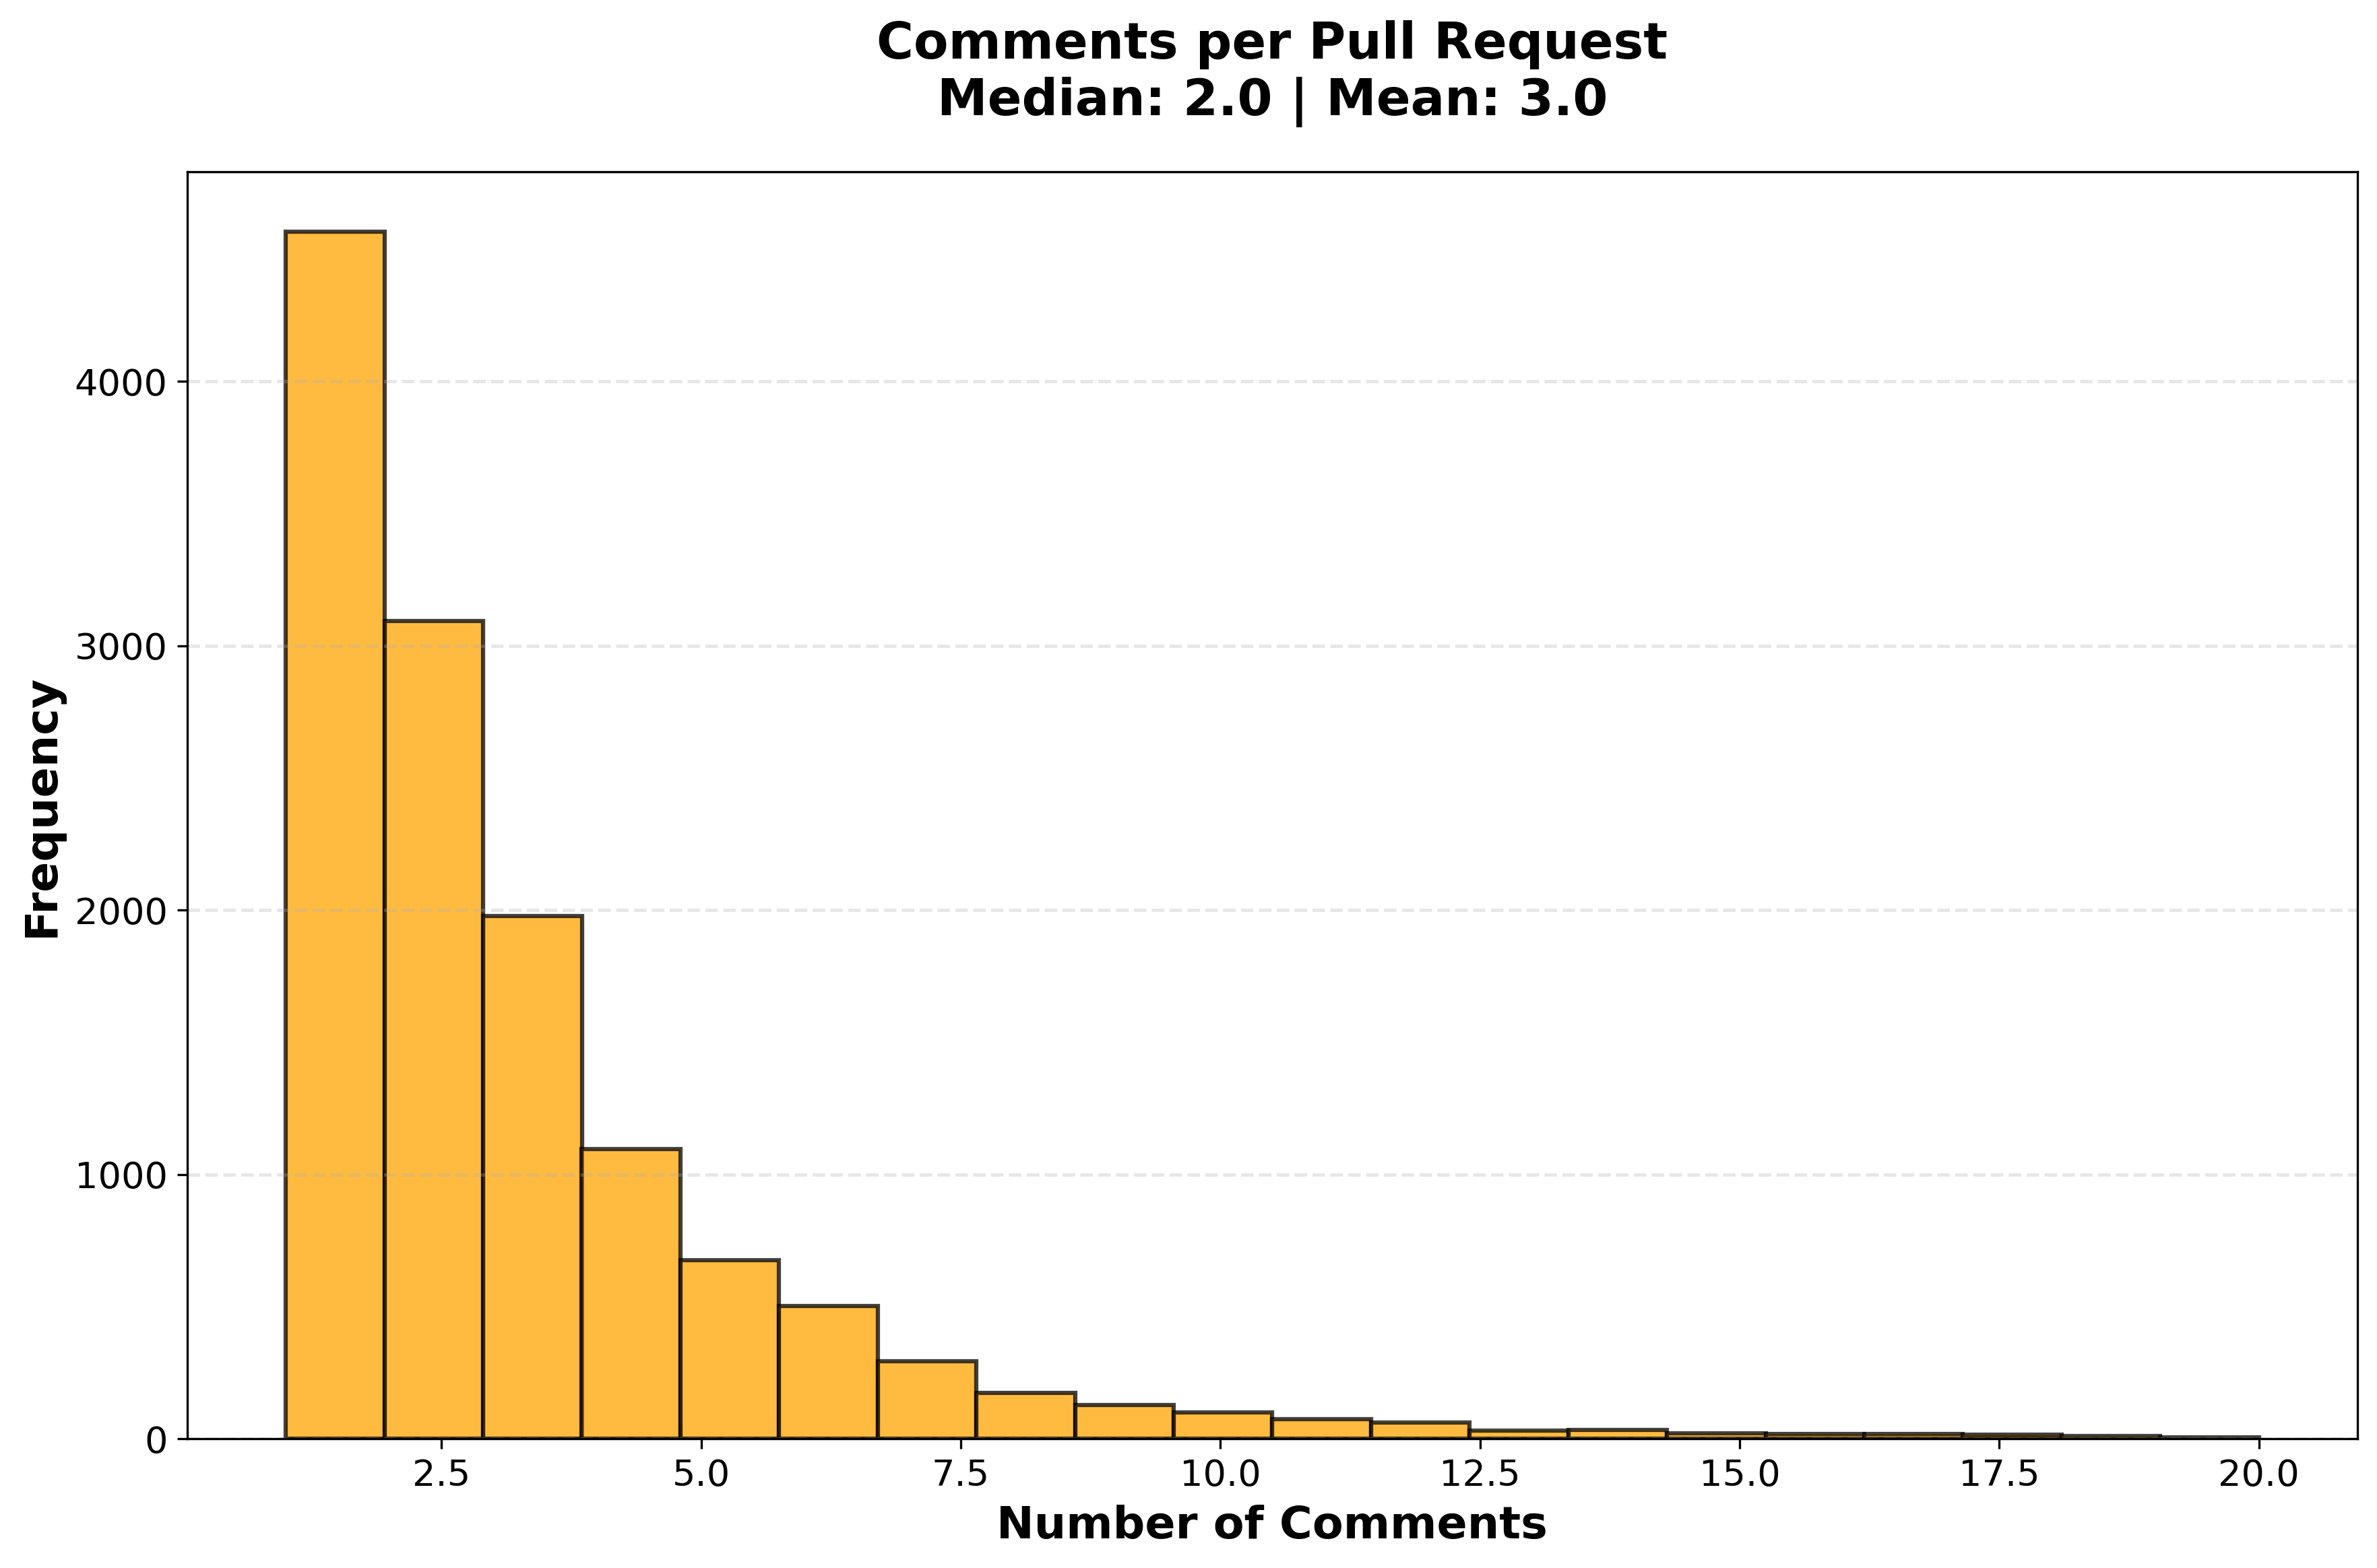
\includegraphics[width=\textwidth]{figures_individual/16_comments_per_pr_histogram.png}
\caption{Comments per PR}
\label{fig:comments}
\end{subfigure}
\hfill
\begin{subfigure}[b]{0.48\textwidth}
\centering
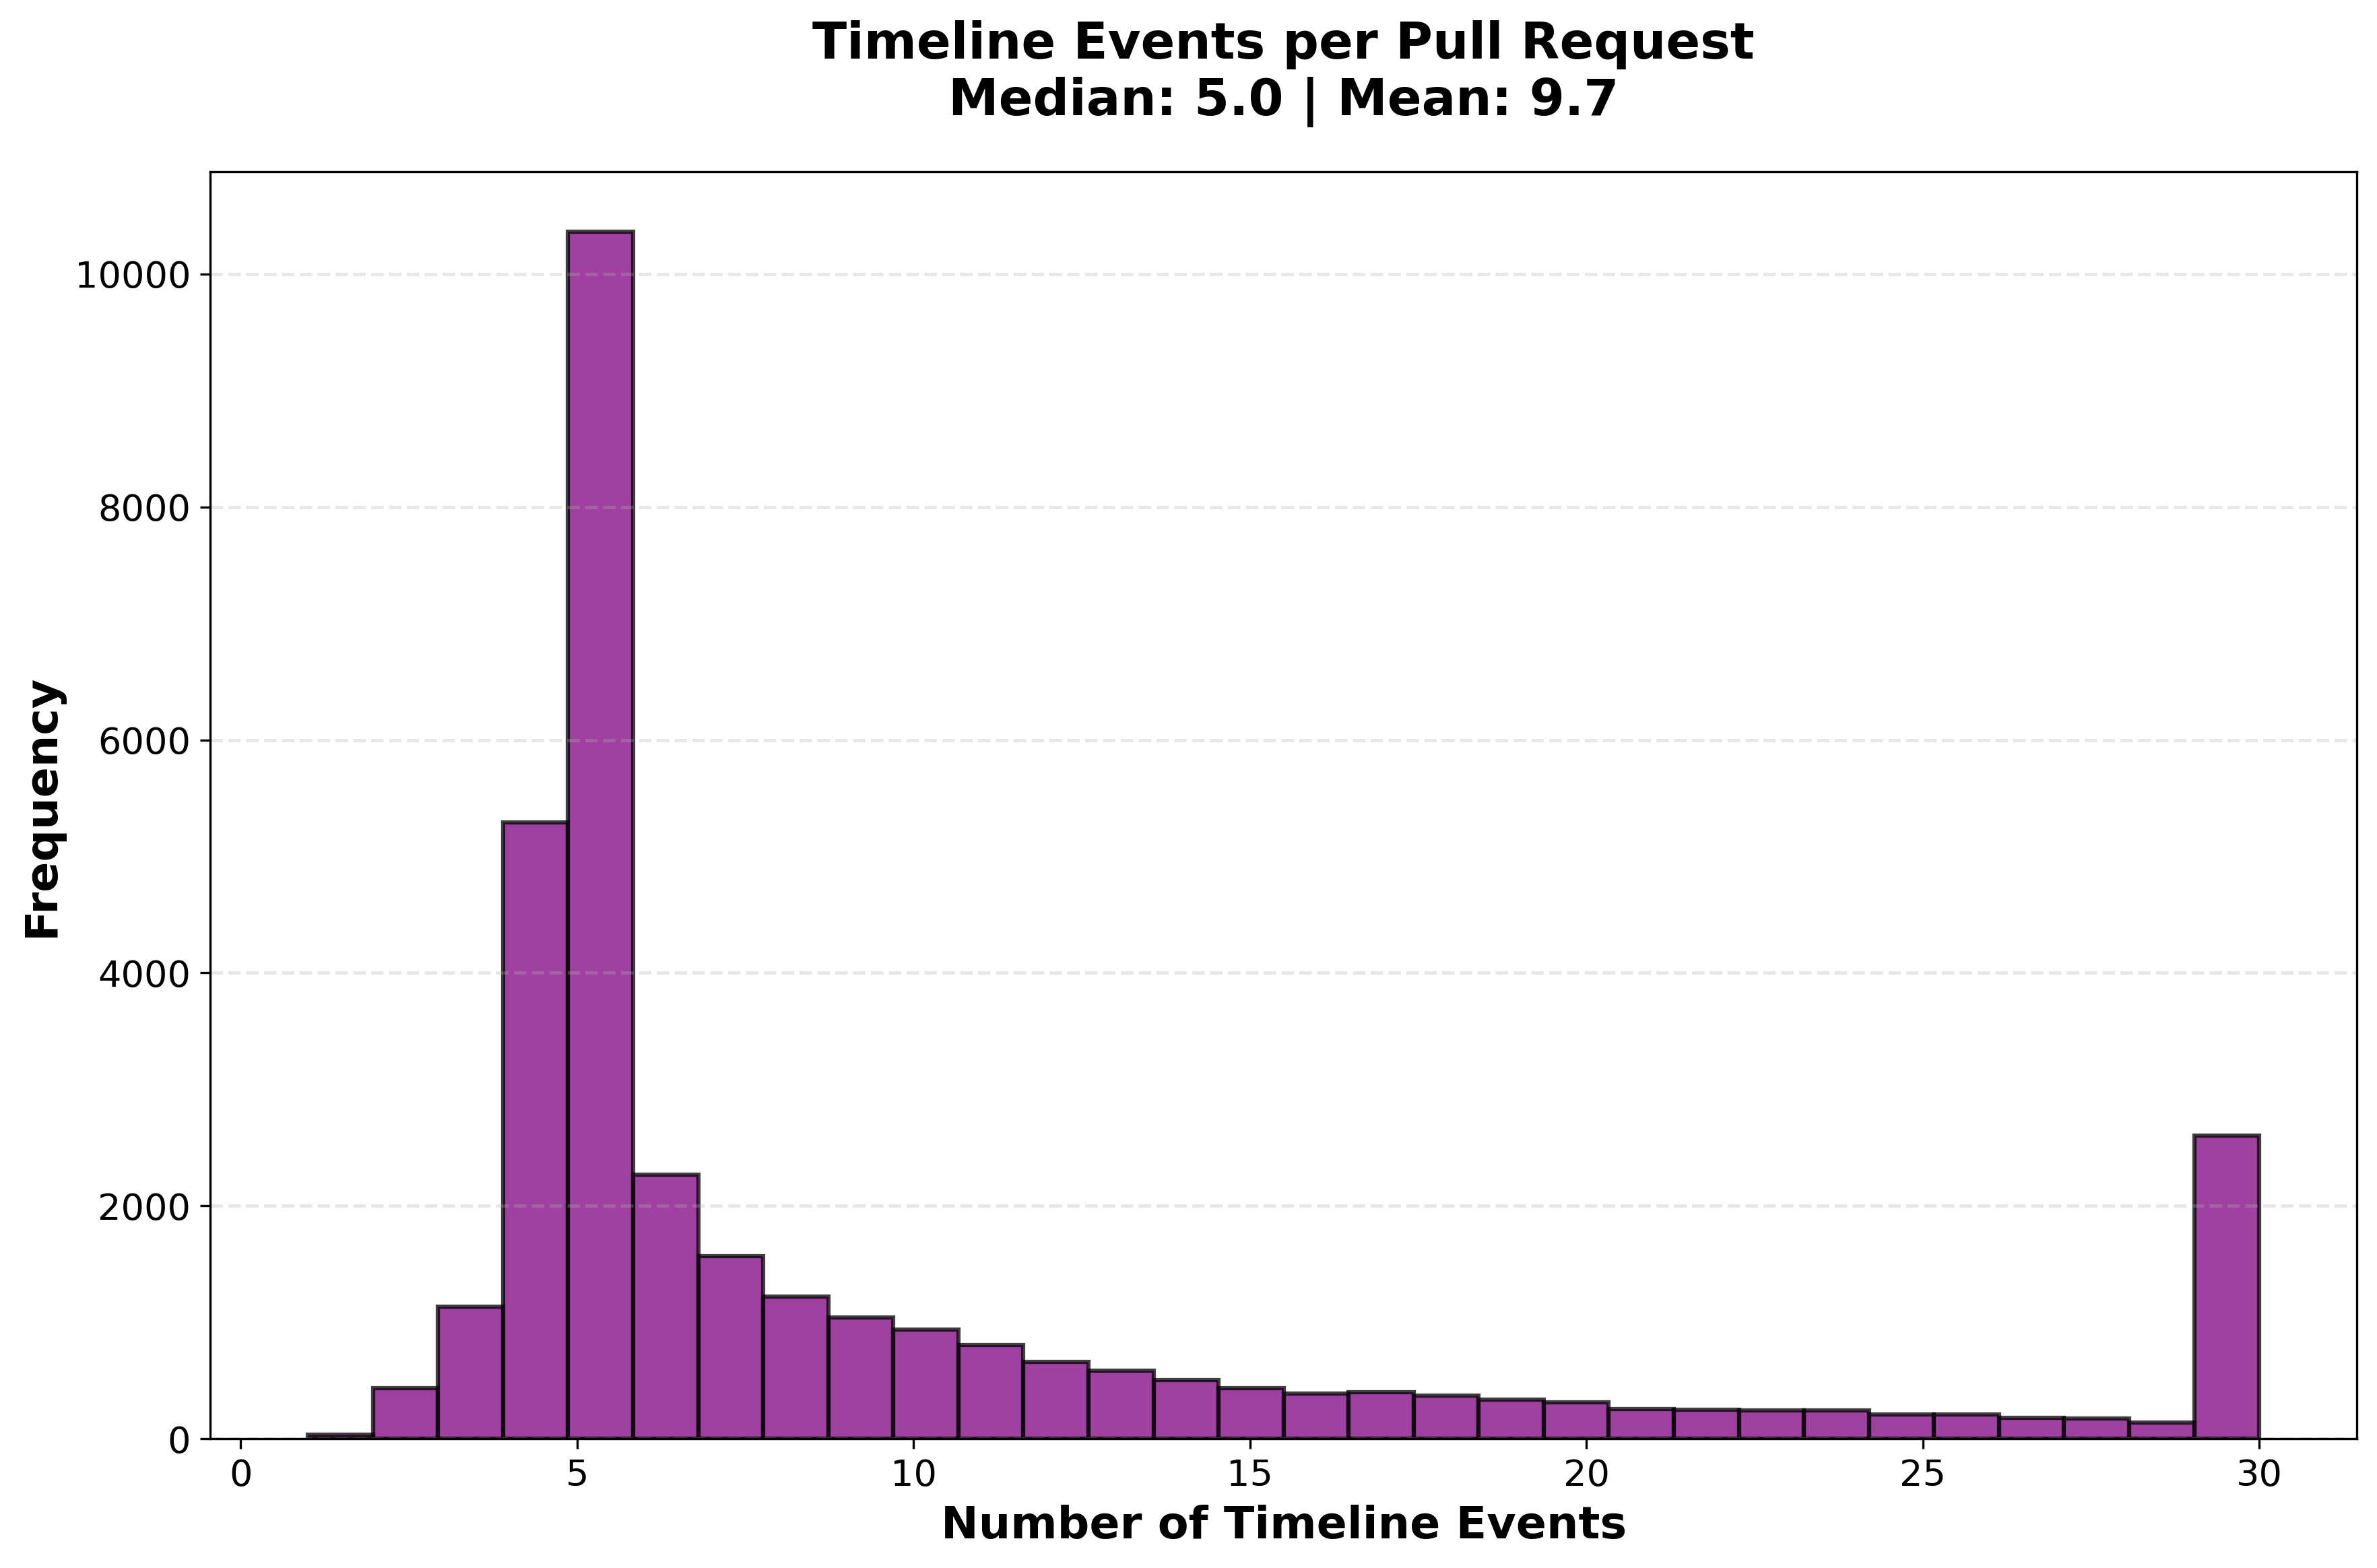
\includegraphics[width=\textwidth]{figures_individual/18_timeline_events_per_pr_histogram.png}
\caption{Timeline events per PR}
\label{fig:timeline}
\end{subfigure}

\caption{Collaborative Activity Distributions (Median: 2-3 commits, 0-1 reviews, 0-1 comments, 9.7 timeline events/PR)}
\label{fig:commit_review_all}
\end{figure}

\subsection{User and Repository Distributions}

Figures~\ref{fig:prs_user}--\ref{fig:languages} show user/repo patterns (TypeScript: 23\%, Python: 19\%).

\begin{figure}[H]
\centering
\begin{subfigure}[b]{0.48\textwidth}
\centering
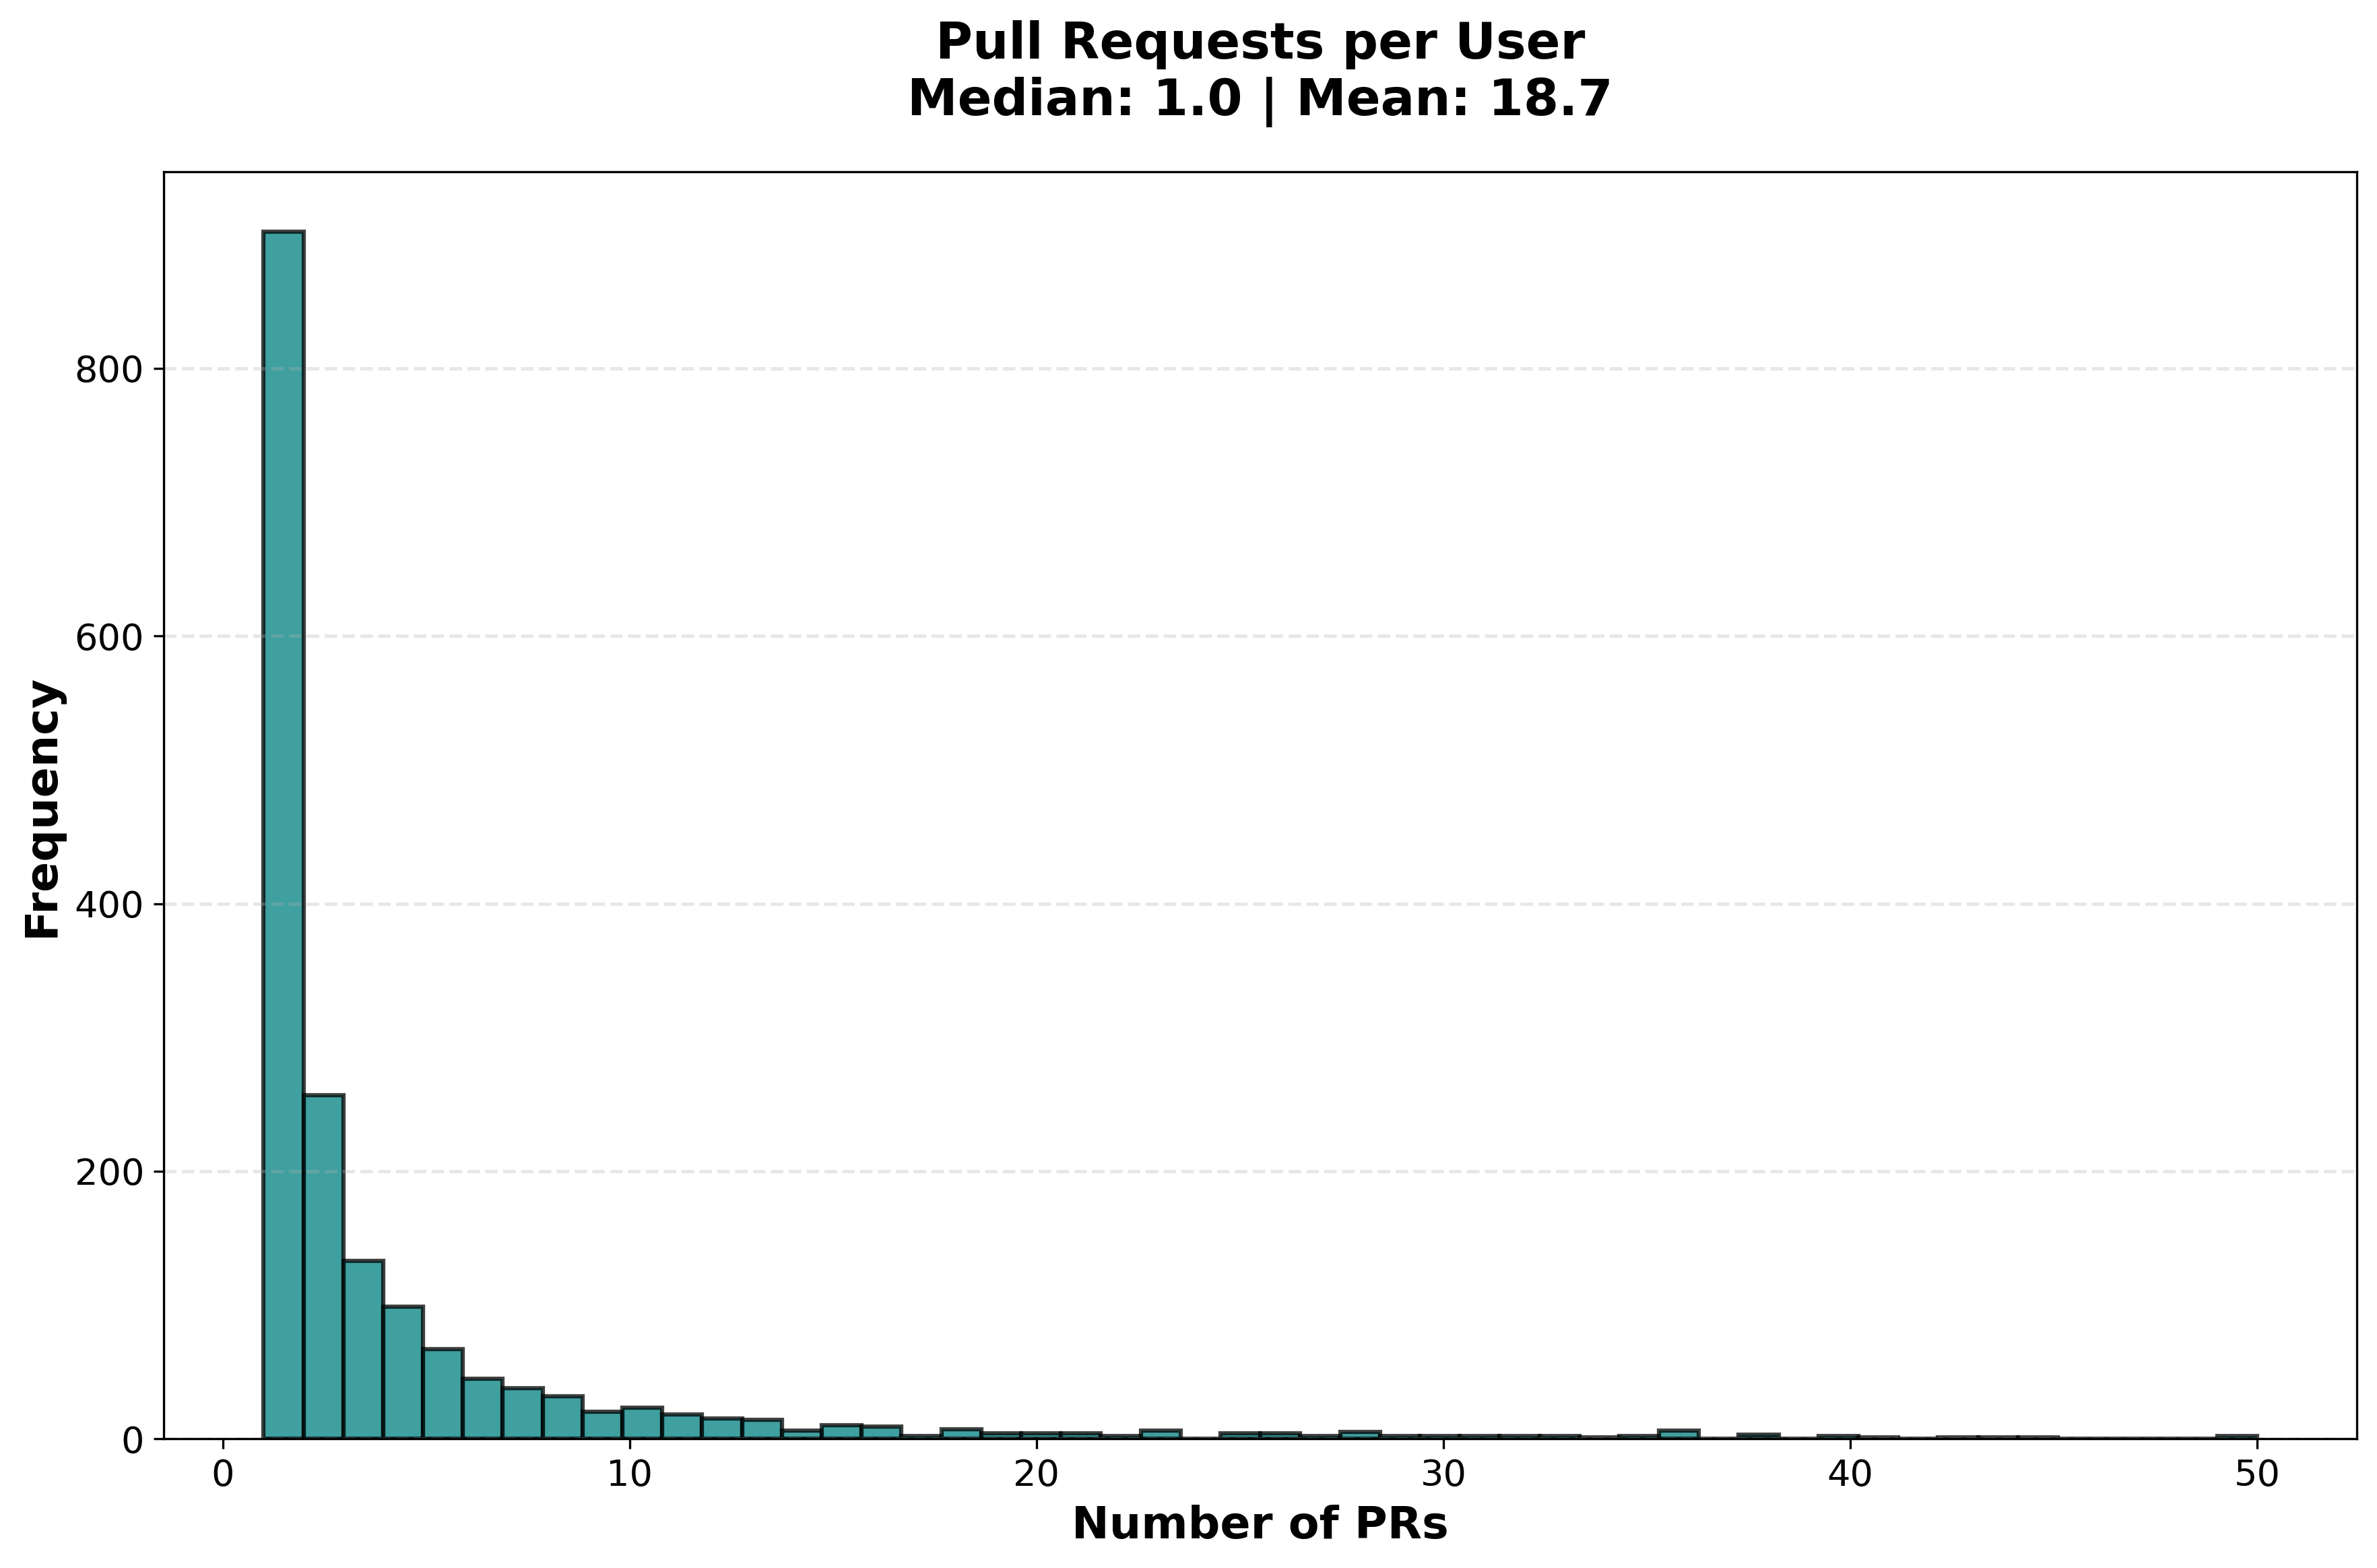
\includegraphics[width=\textwidth]{figures_individual/19_prs_per_user_histogram.png}
\caption{PRs per user}
\label{fig:prs_user}
\end{subfigure}
\hfill
\begin{subfigure}[b]{0.48\textwidth}
\centering
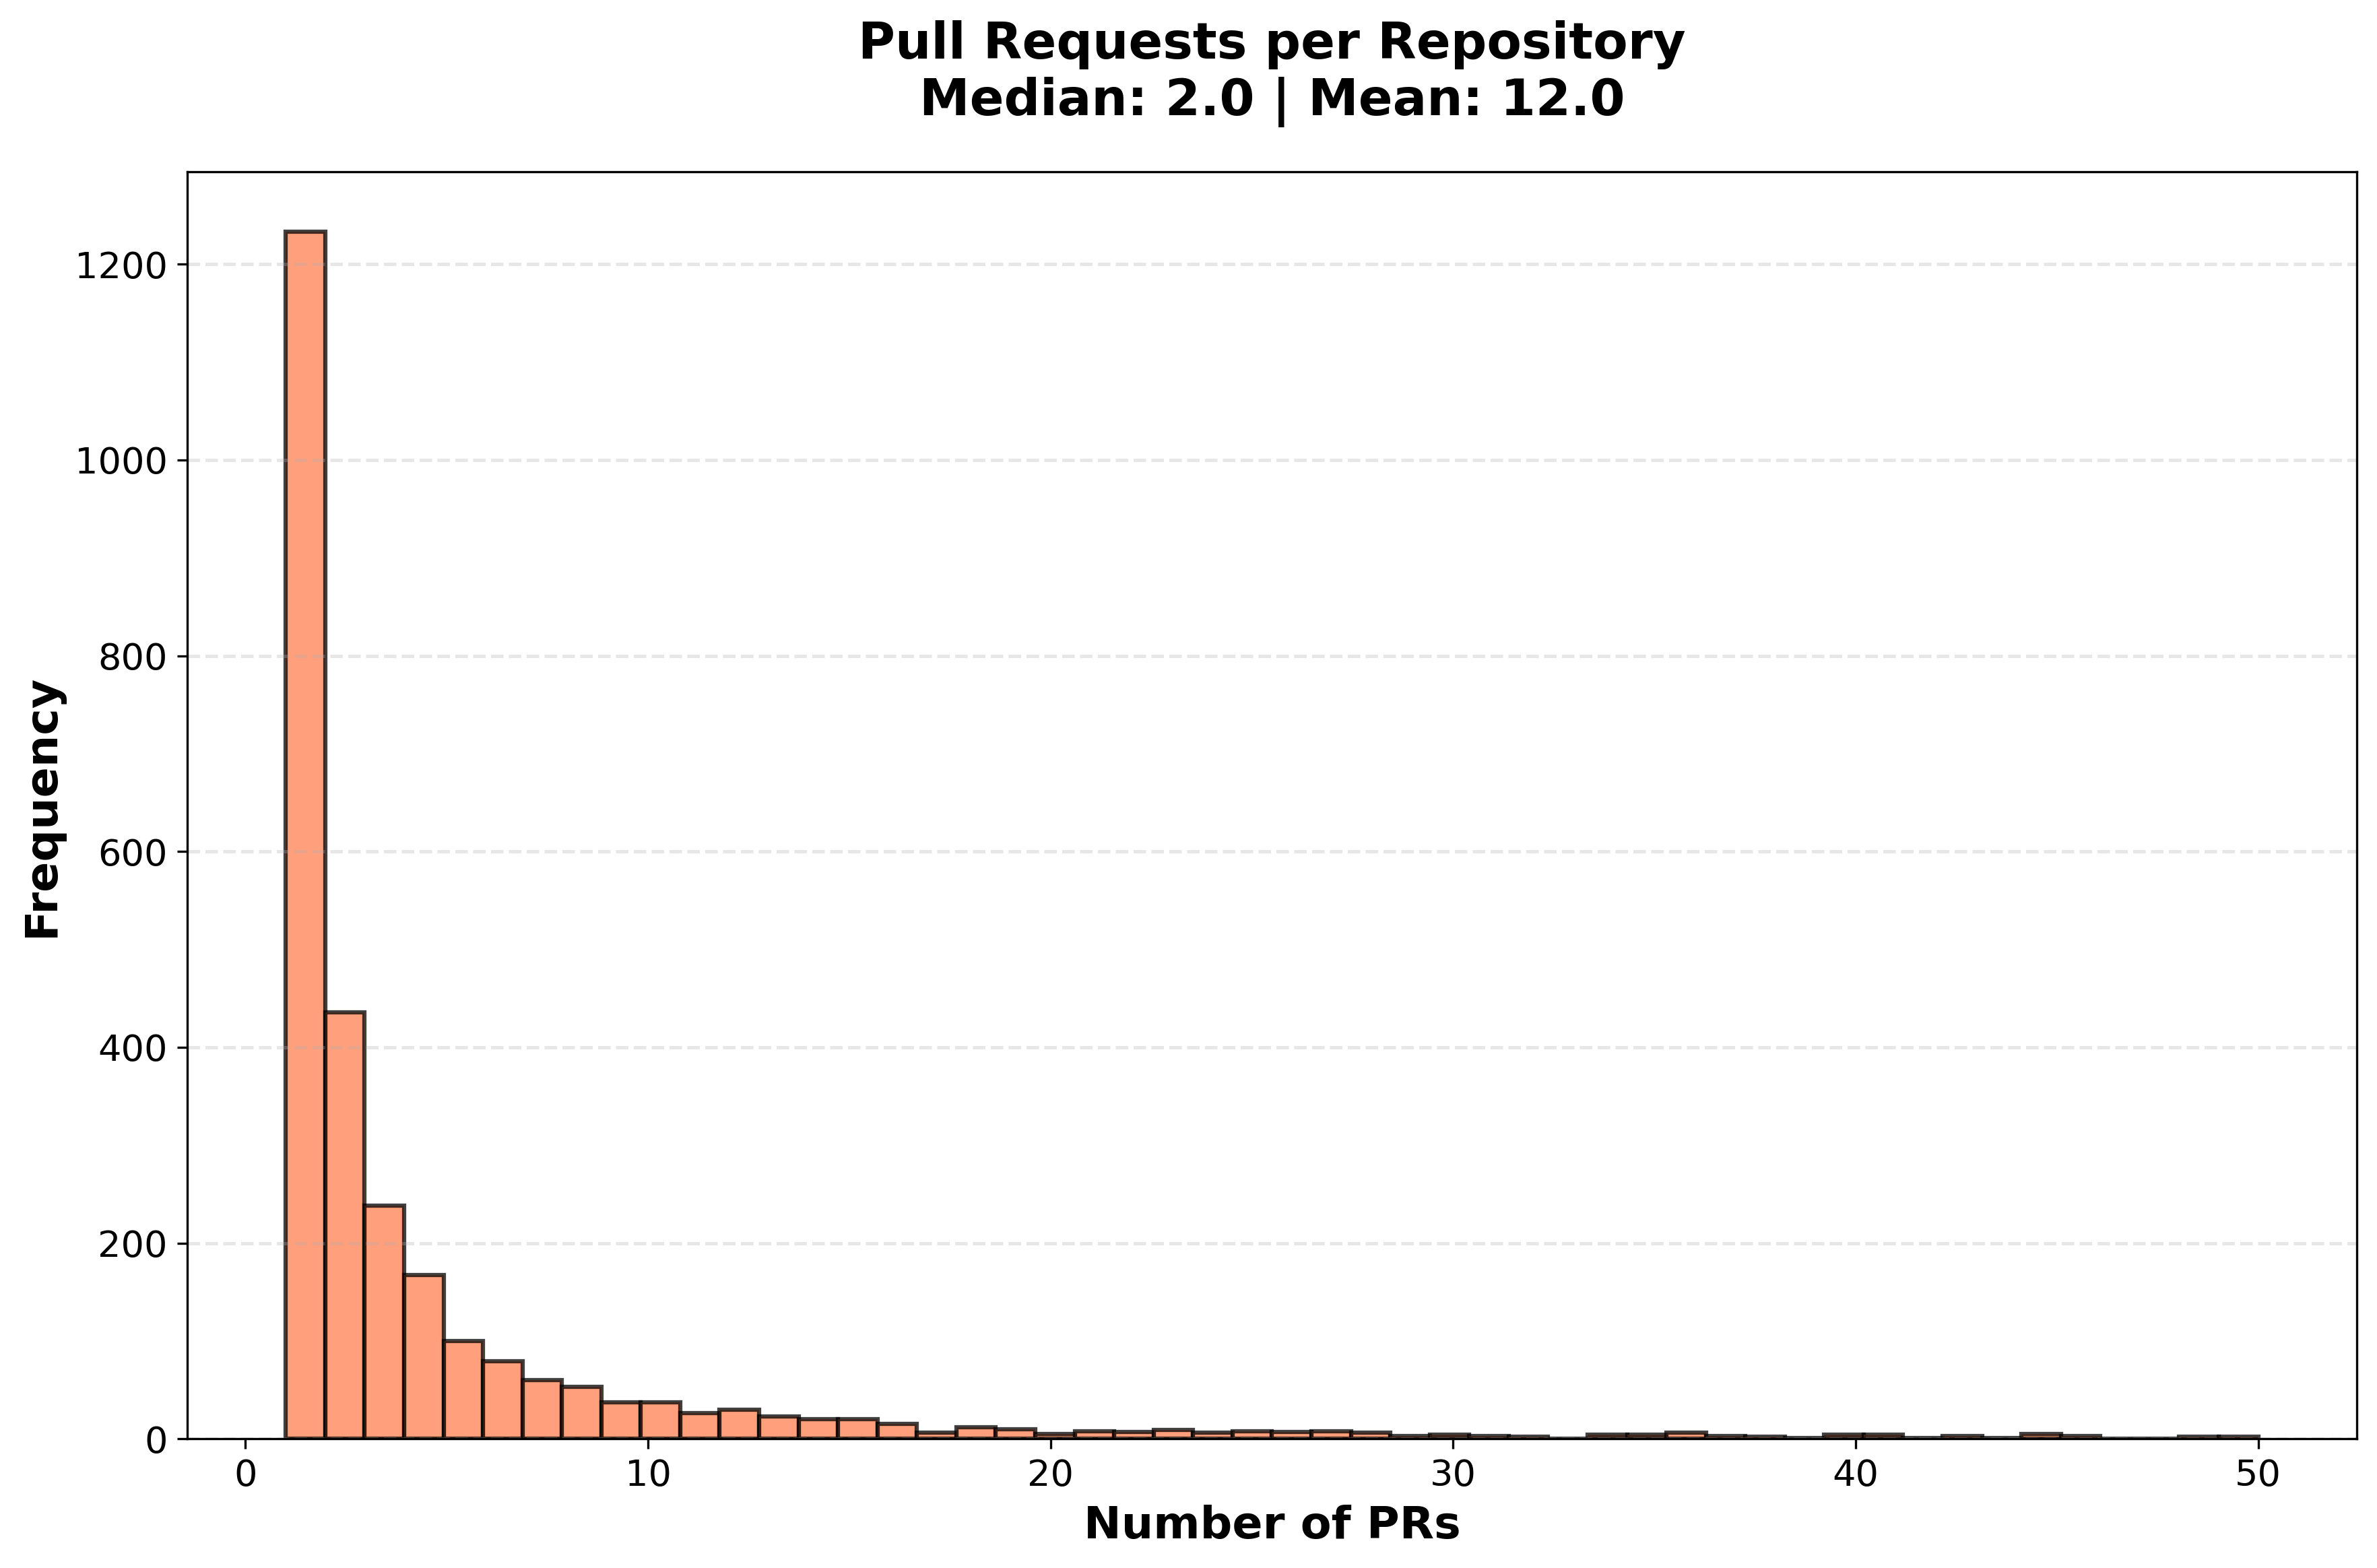
\includegraphics[width=\textwidth]{figures_individual/20_prs_per_repo_histogram.png}
\caption{PRs per repository}
\label{fig:prs_repo}
\end{subfigure}

\vspace{0.3cm}

\begin{subfigure}[b]{0.48\textwidth}
\centering
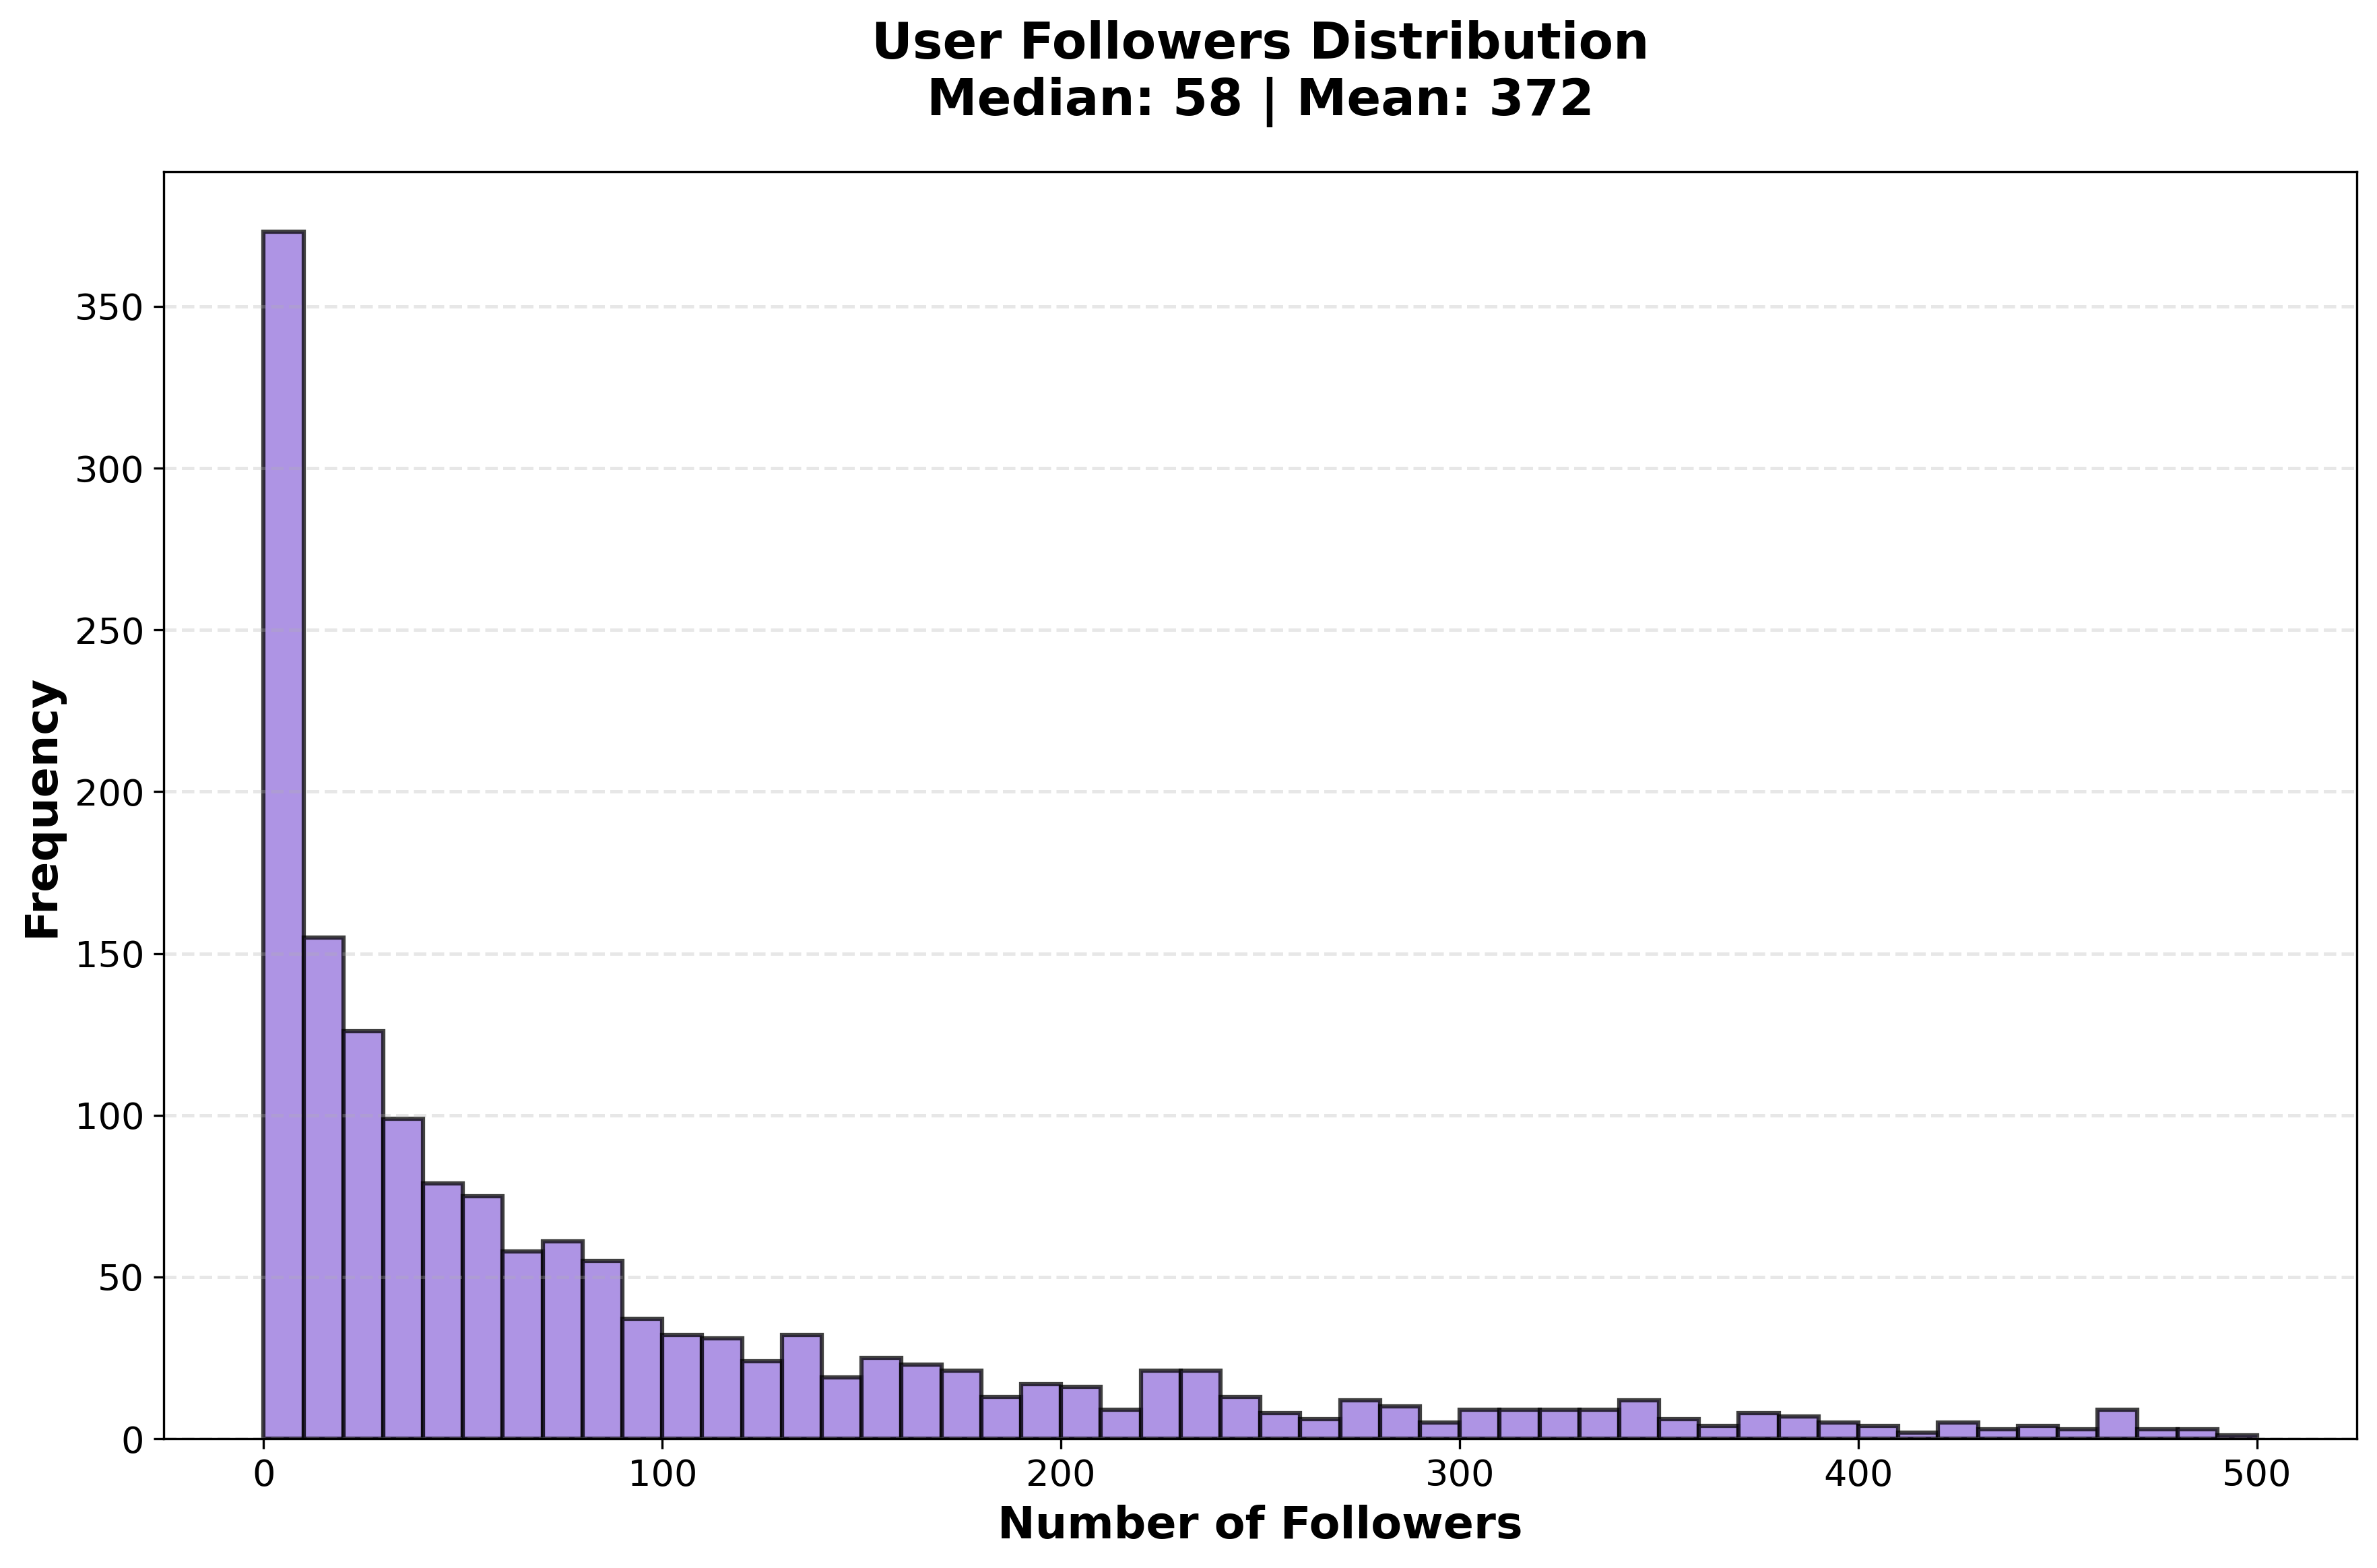
\includegraphics[width=\textwidth]{figures_individual/21_user_followers_histogram.png}
\caption{User followers distribution}
\label{fig:followers}
\end{subfigure}
\hfill
\begin{subfigure}[b]{0.48\textwidth}
\centering
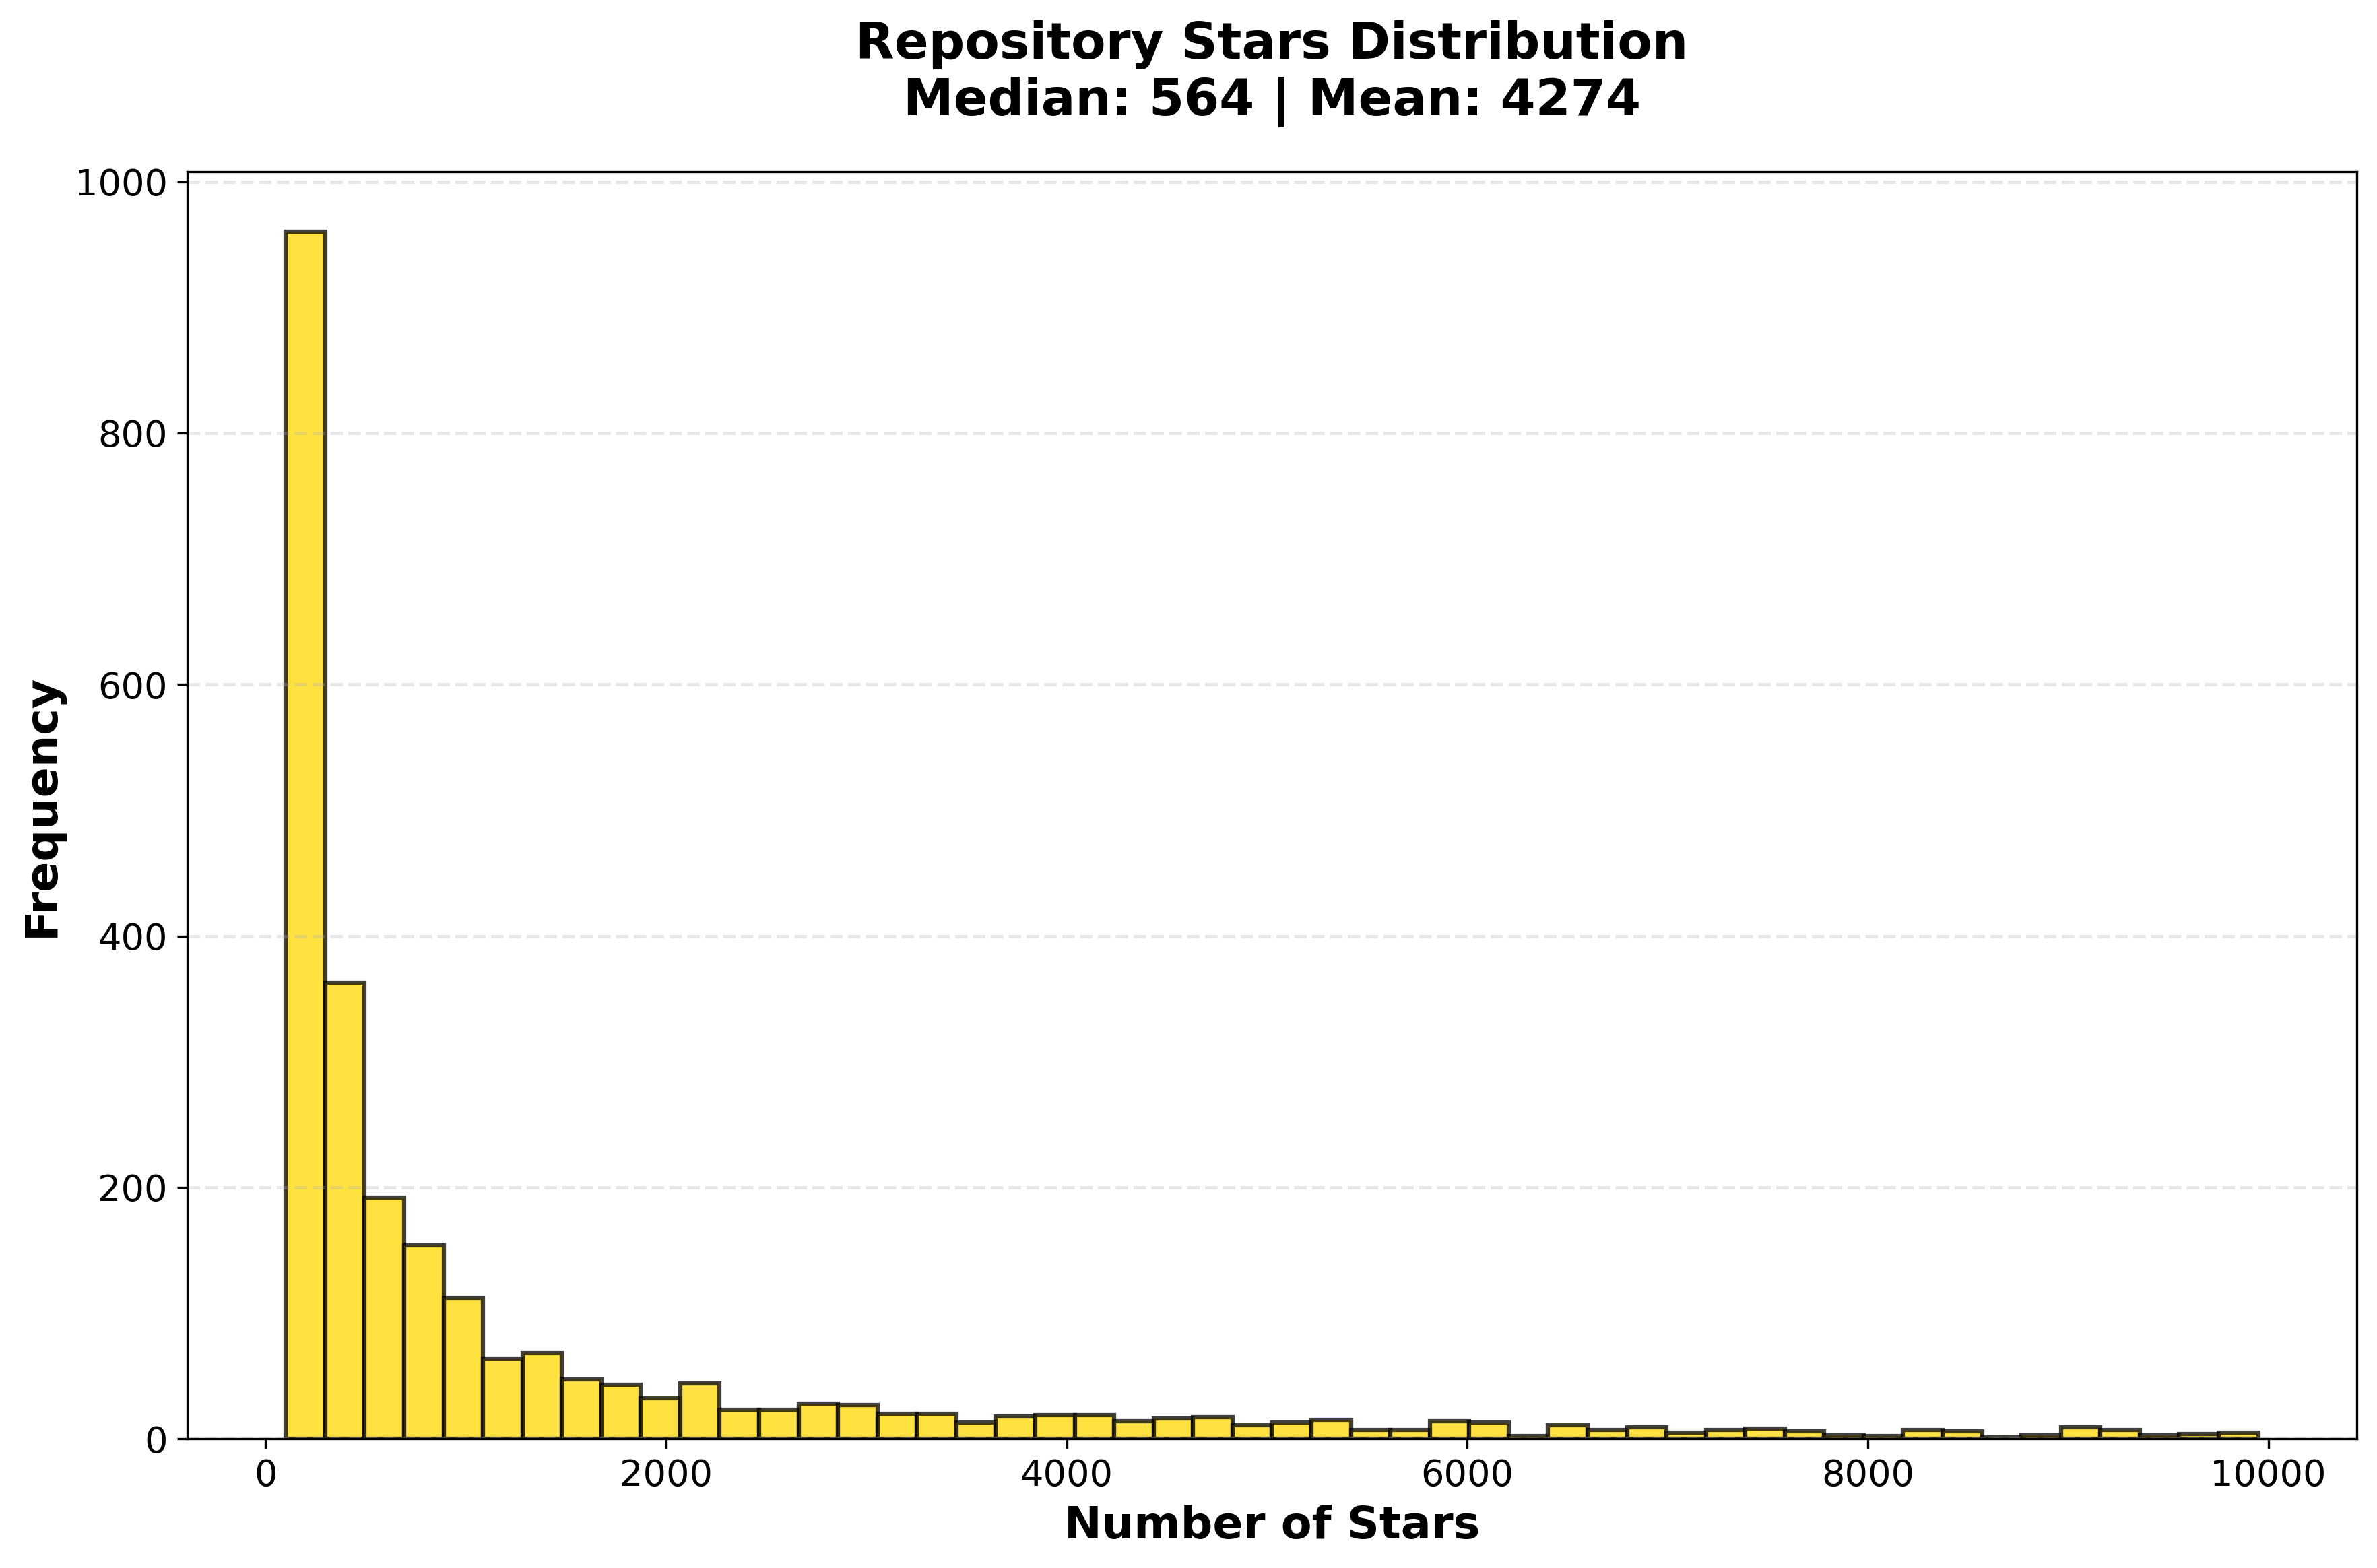
\includegraphics[width=\textwidth]{figures_individual/22_repo_stars_histogram.png}
\caption{Repository stars distribution}
\label{fig:stars}
\end{subfigure}

\vspace{0.3cm}

\begin{subfigure}[b]{0.9\textwidth}
\centering
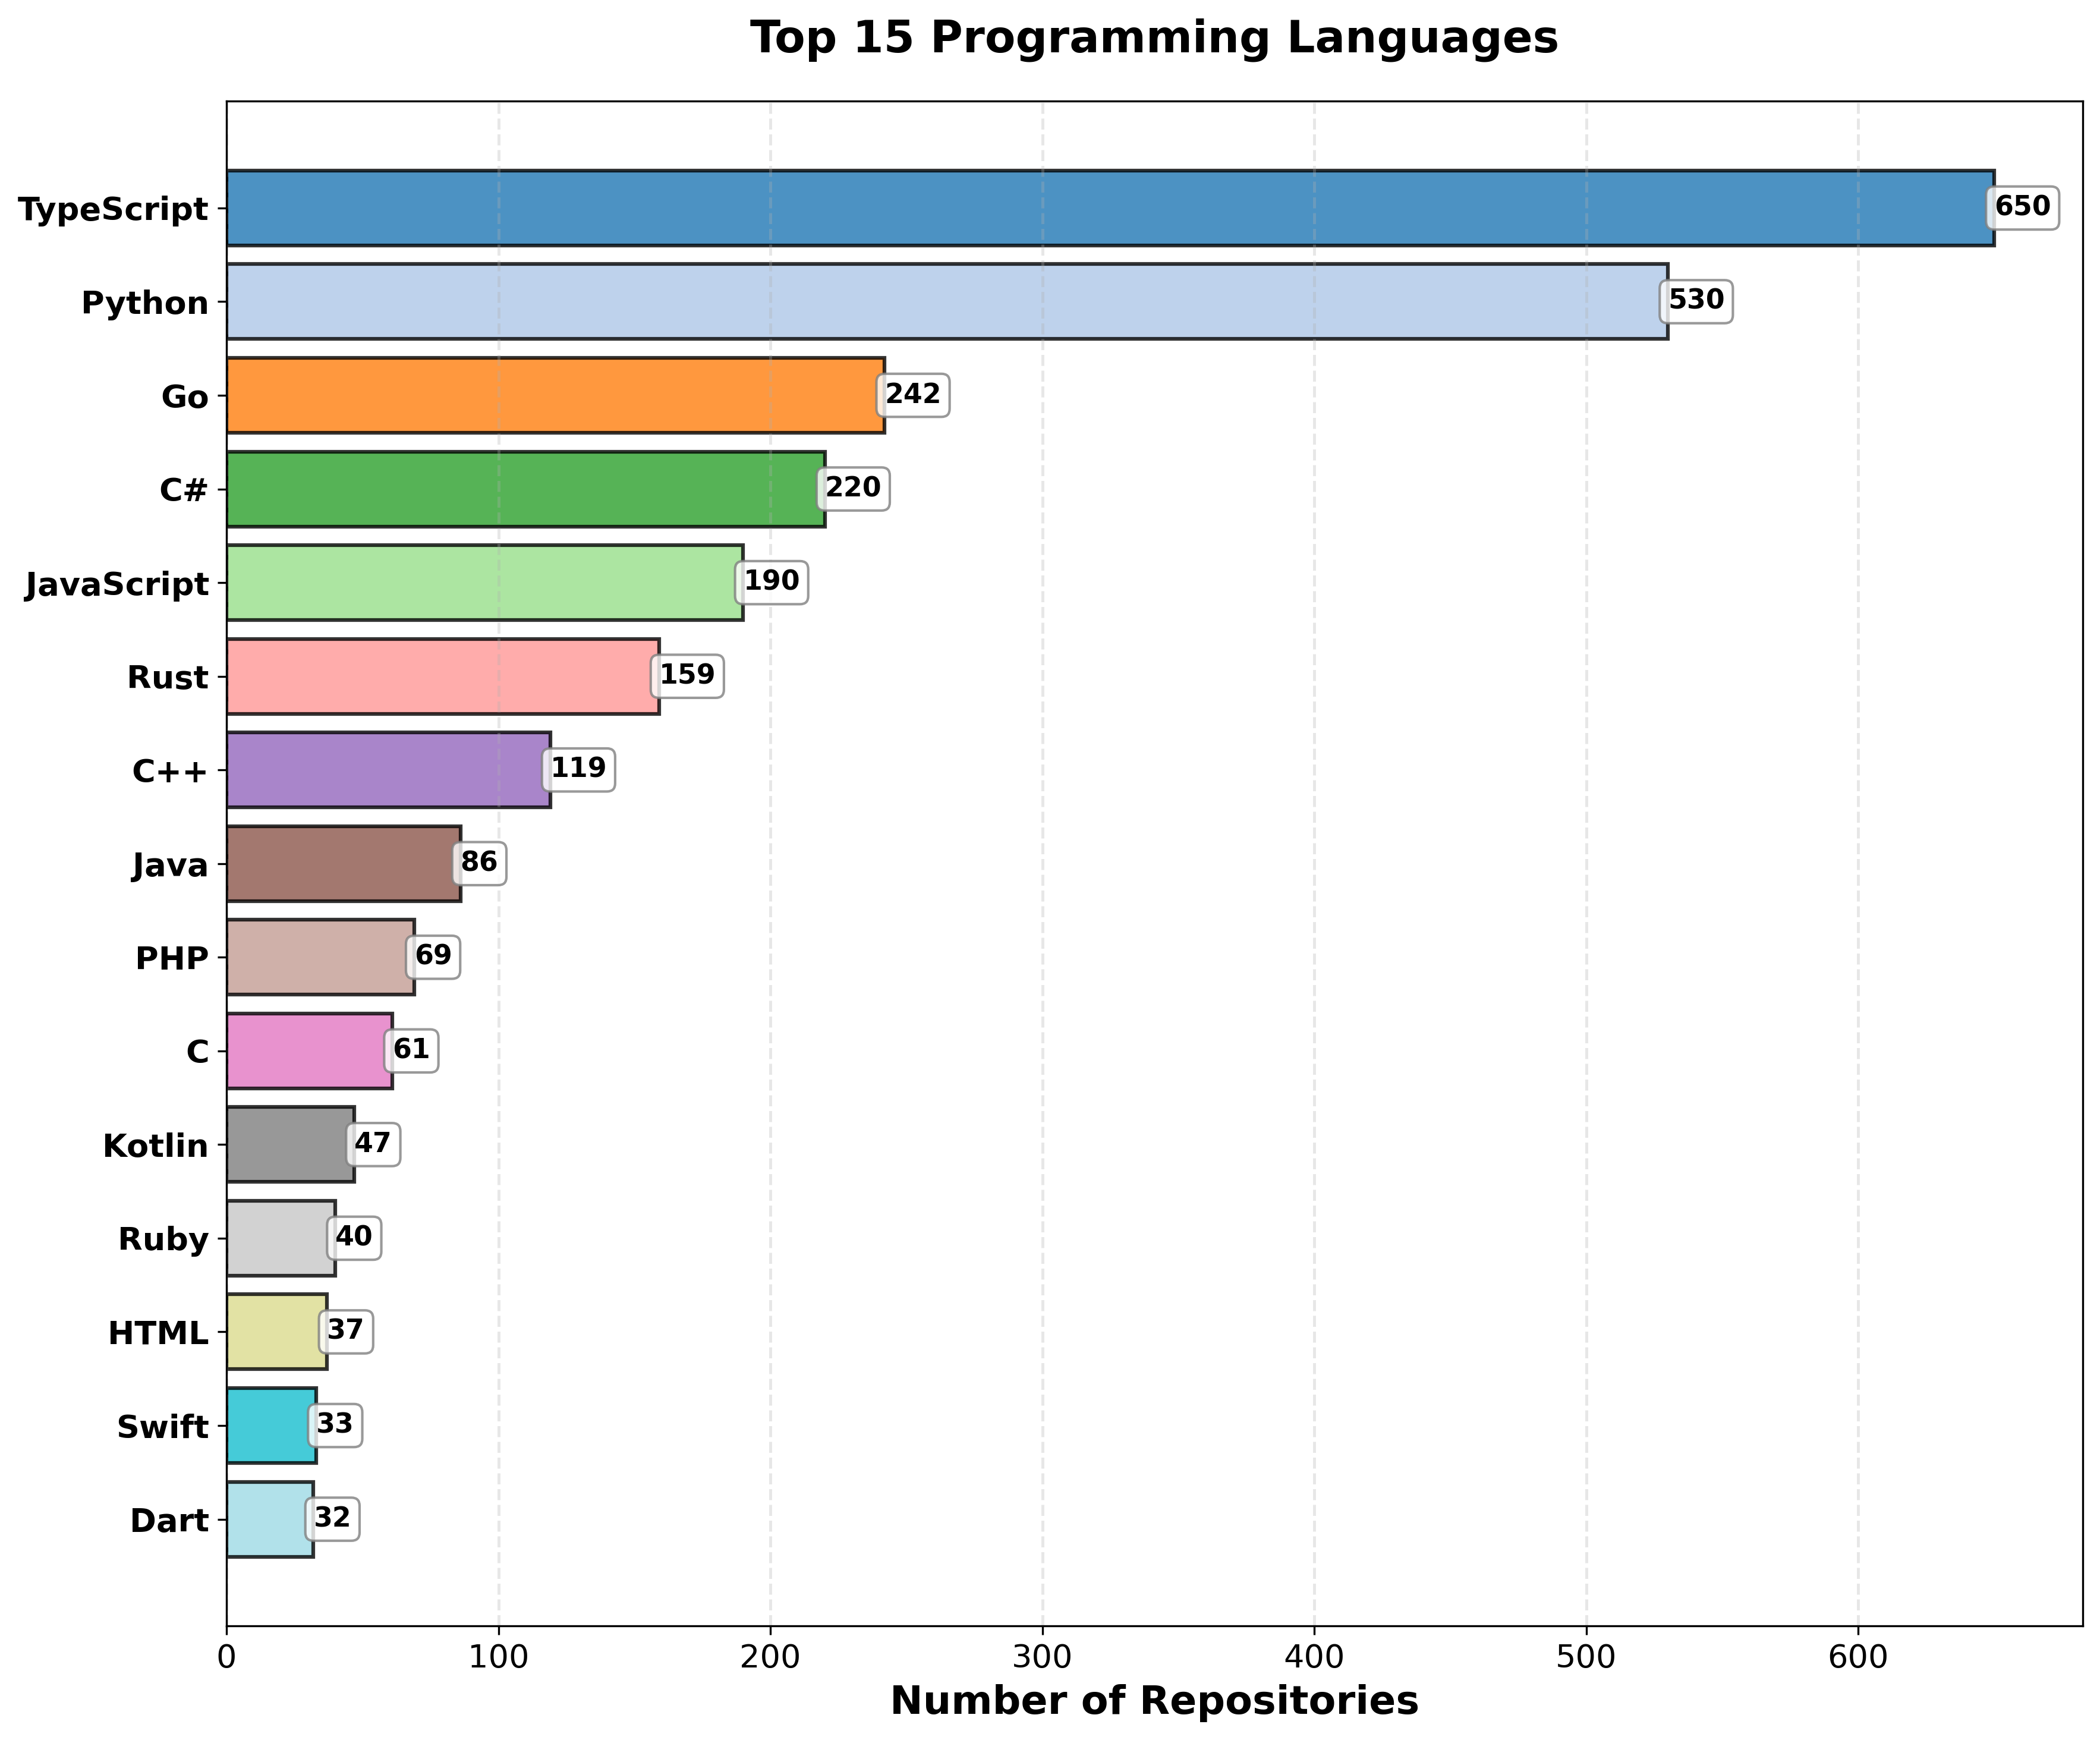
\includegraphics[width=\textwidth]{figures_individual/24_programming_languages_barplot.png}
\caption{Top 15 programming languages across repositories}
\label{fig:languages}
\end{subfigure}

\caption{User and Repository Distributions (Median: 18.7 PRs/user, 12.0 PRs/repo, 58 followers, 564 stars)}
\label{fig:user_repo_all}
\end{figure}

\subsection{File-Level Change Distributions}

Figures~\ref{fig:file_adds}--\ref{fig:event_types} show file-level changes (Median: 4 additions, 1 deletion per file).

\begin{figure}[H]
\centering
\begin{subfigure}[b]{0.48\textwidth}
\centering
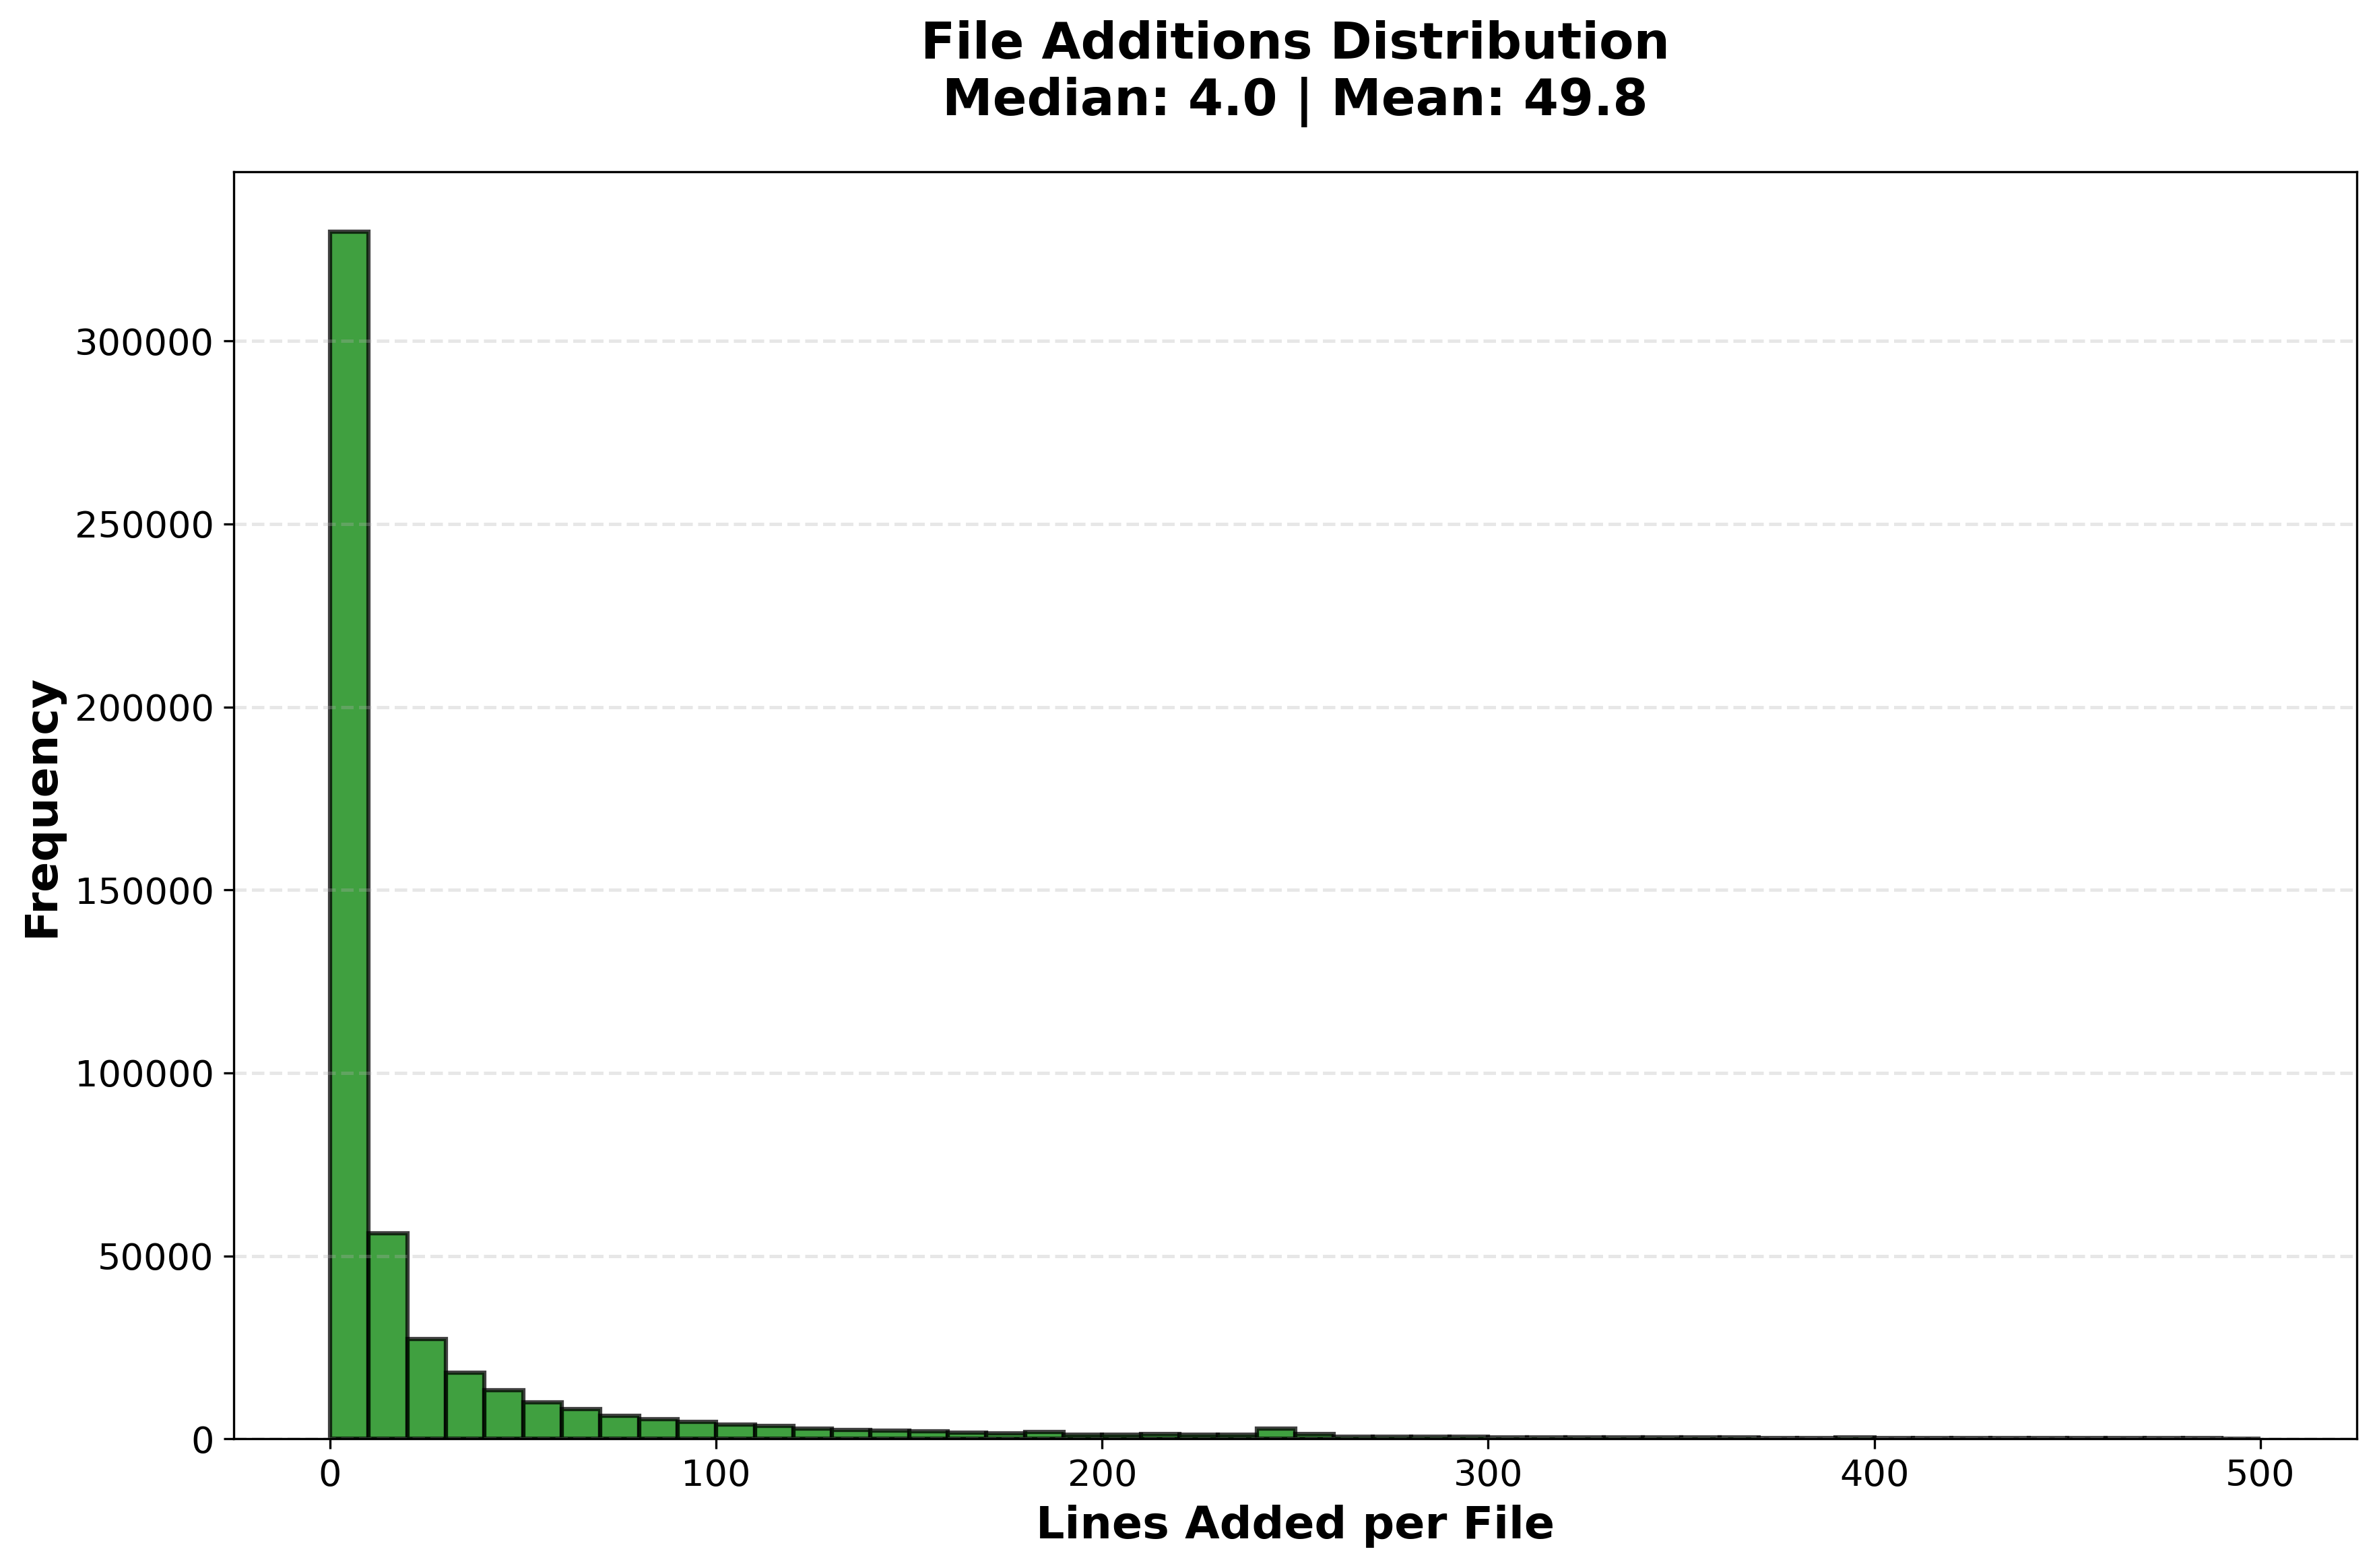
\includegraphics[width=\textwidth]{figures_individual/25_file_additions_histogram.png}
\caption{Lines added per file}
\label{fig:file_adds}
\end{subfigure}
\hfill
\begin{subfigure}[b]{0.48\textwidth}
\centering
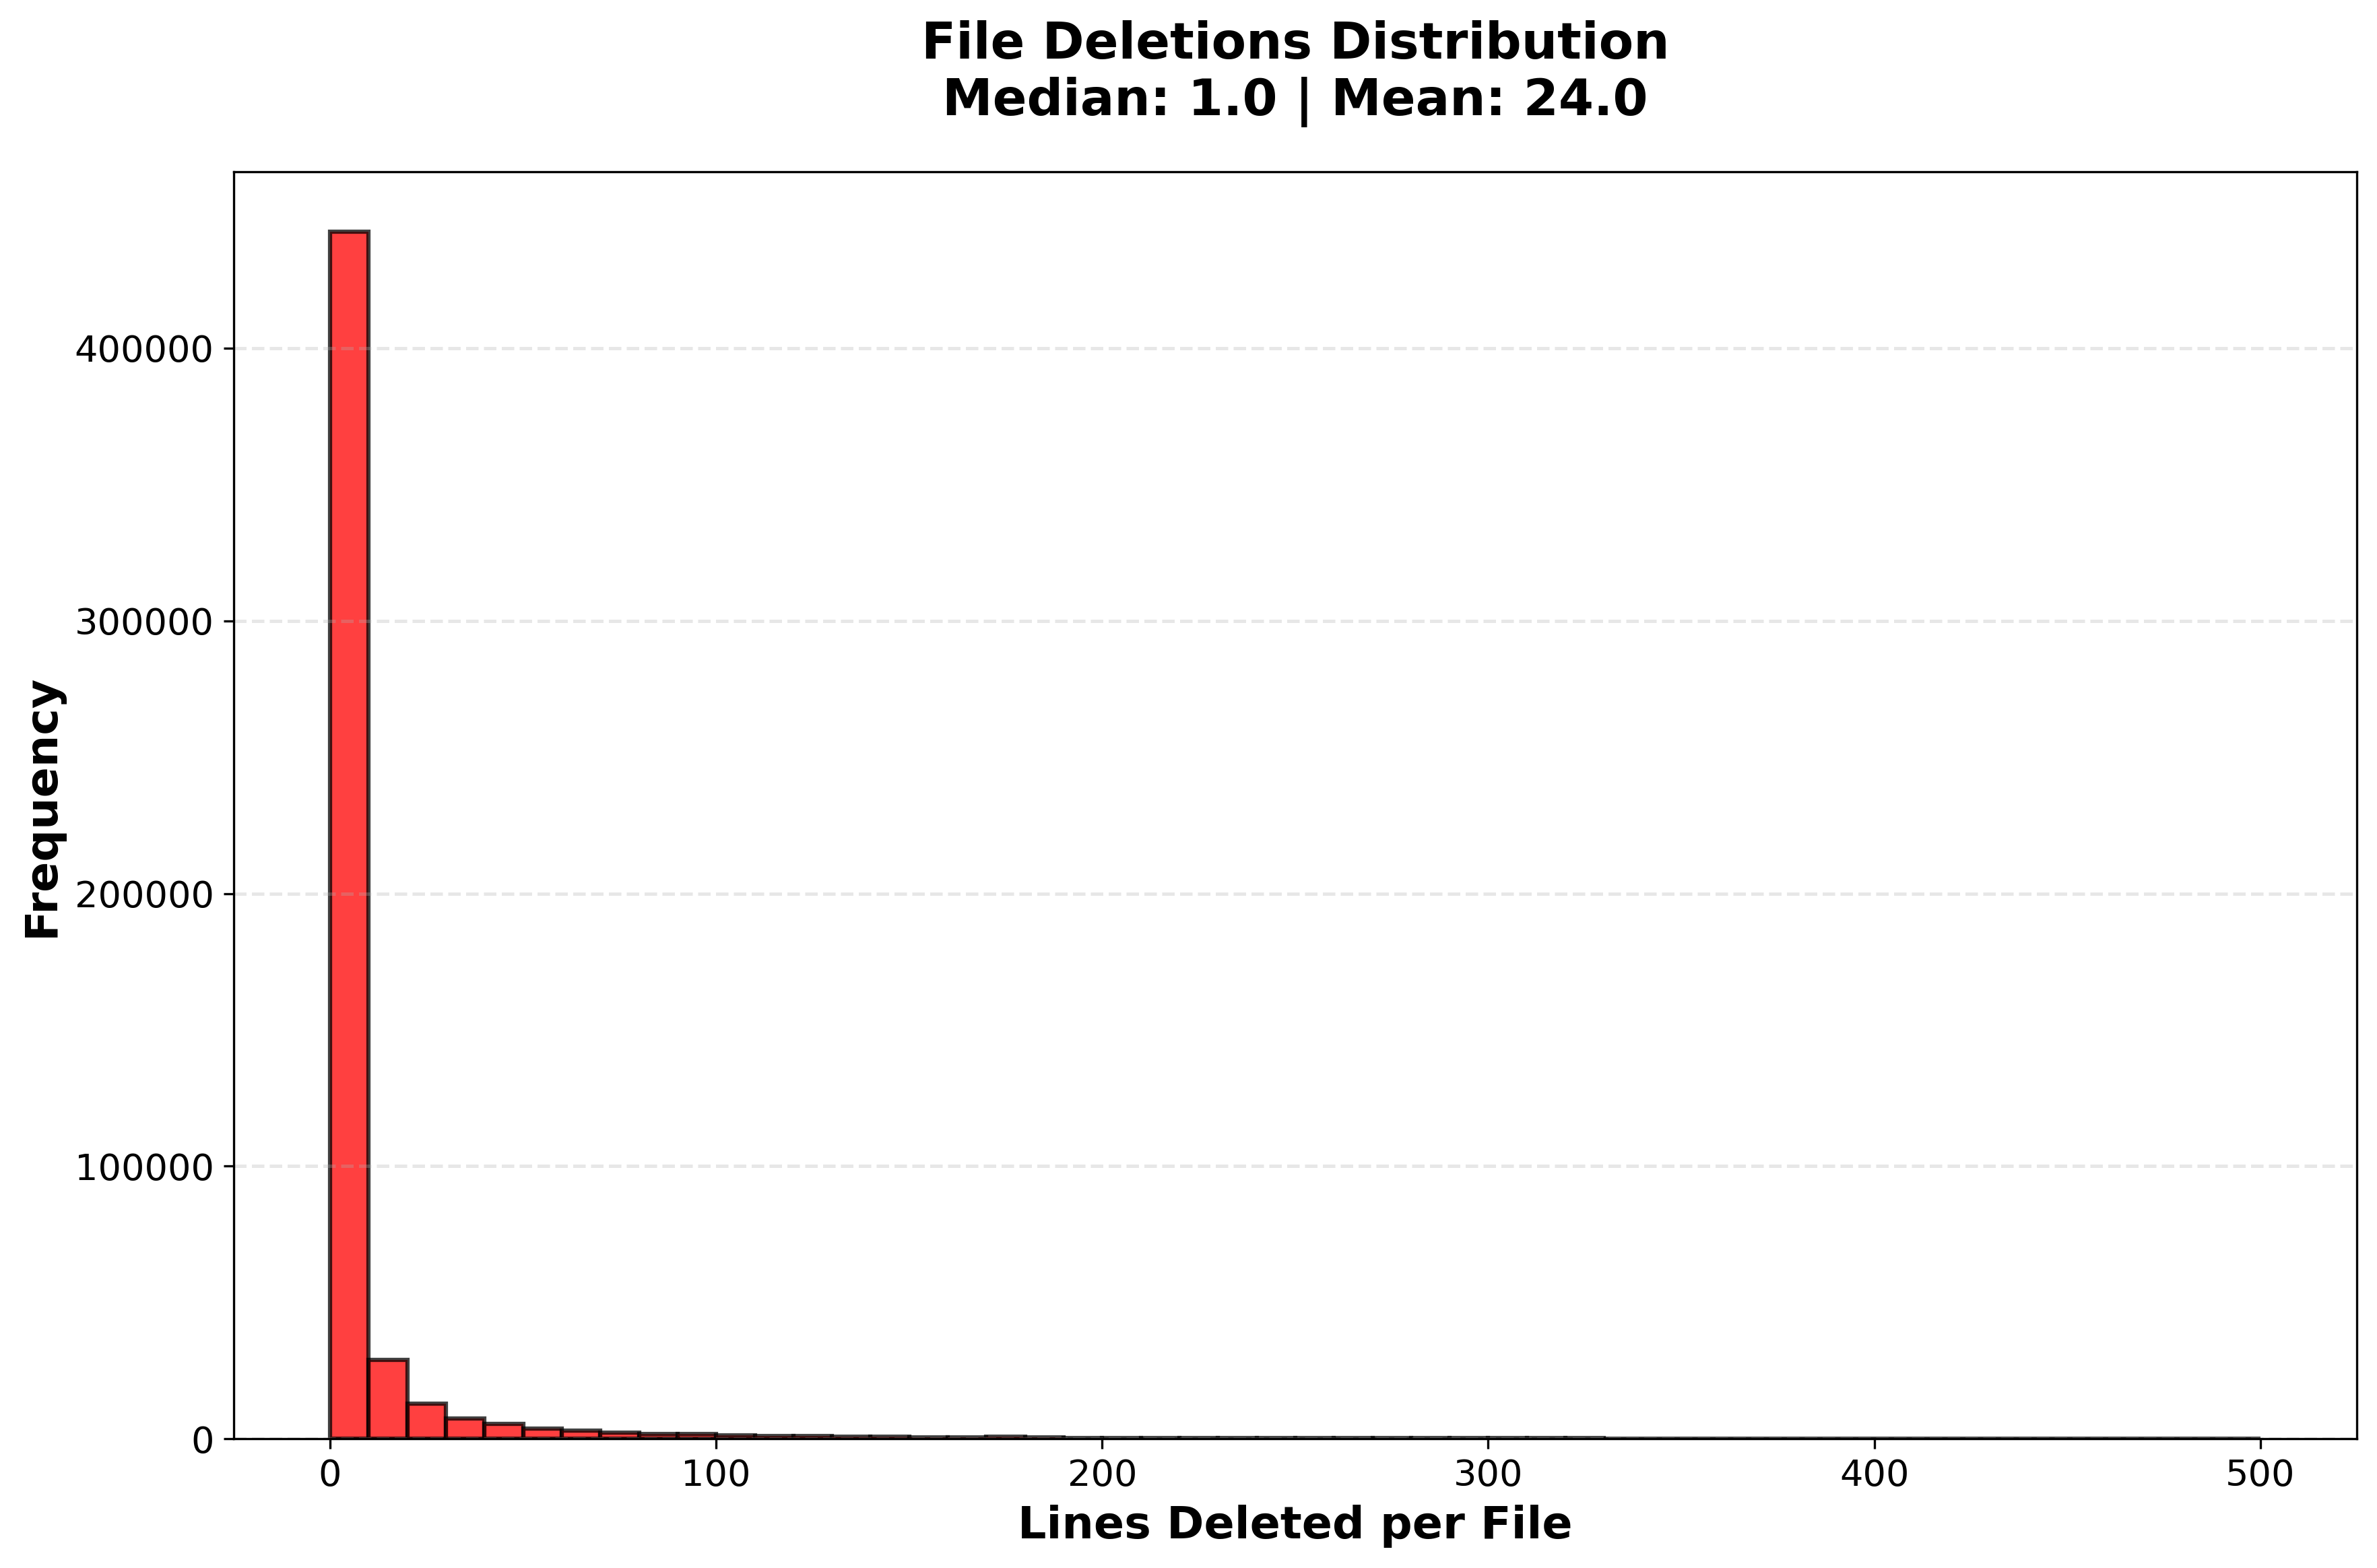
\includegraphics[width=\textwidth]{figures_individual/26_file_deletions_histogram.png}
\caption{Lines deleted per file}
\label{fig:file_dels}
\end{subfigure}

\vspace{0.3cm}

\begin{subfigure}[b]{0.48\textwidth}
\centering
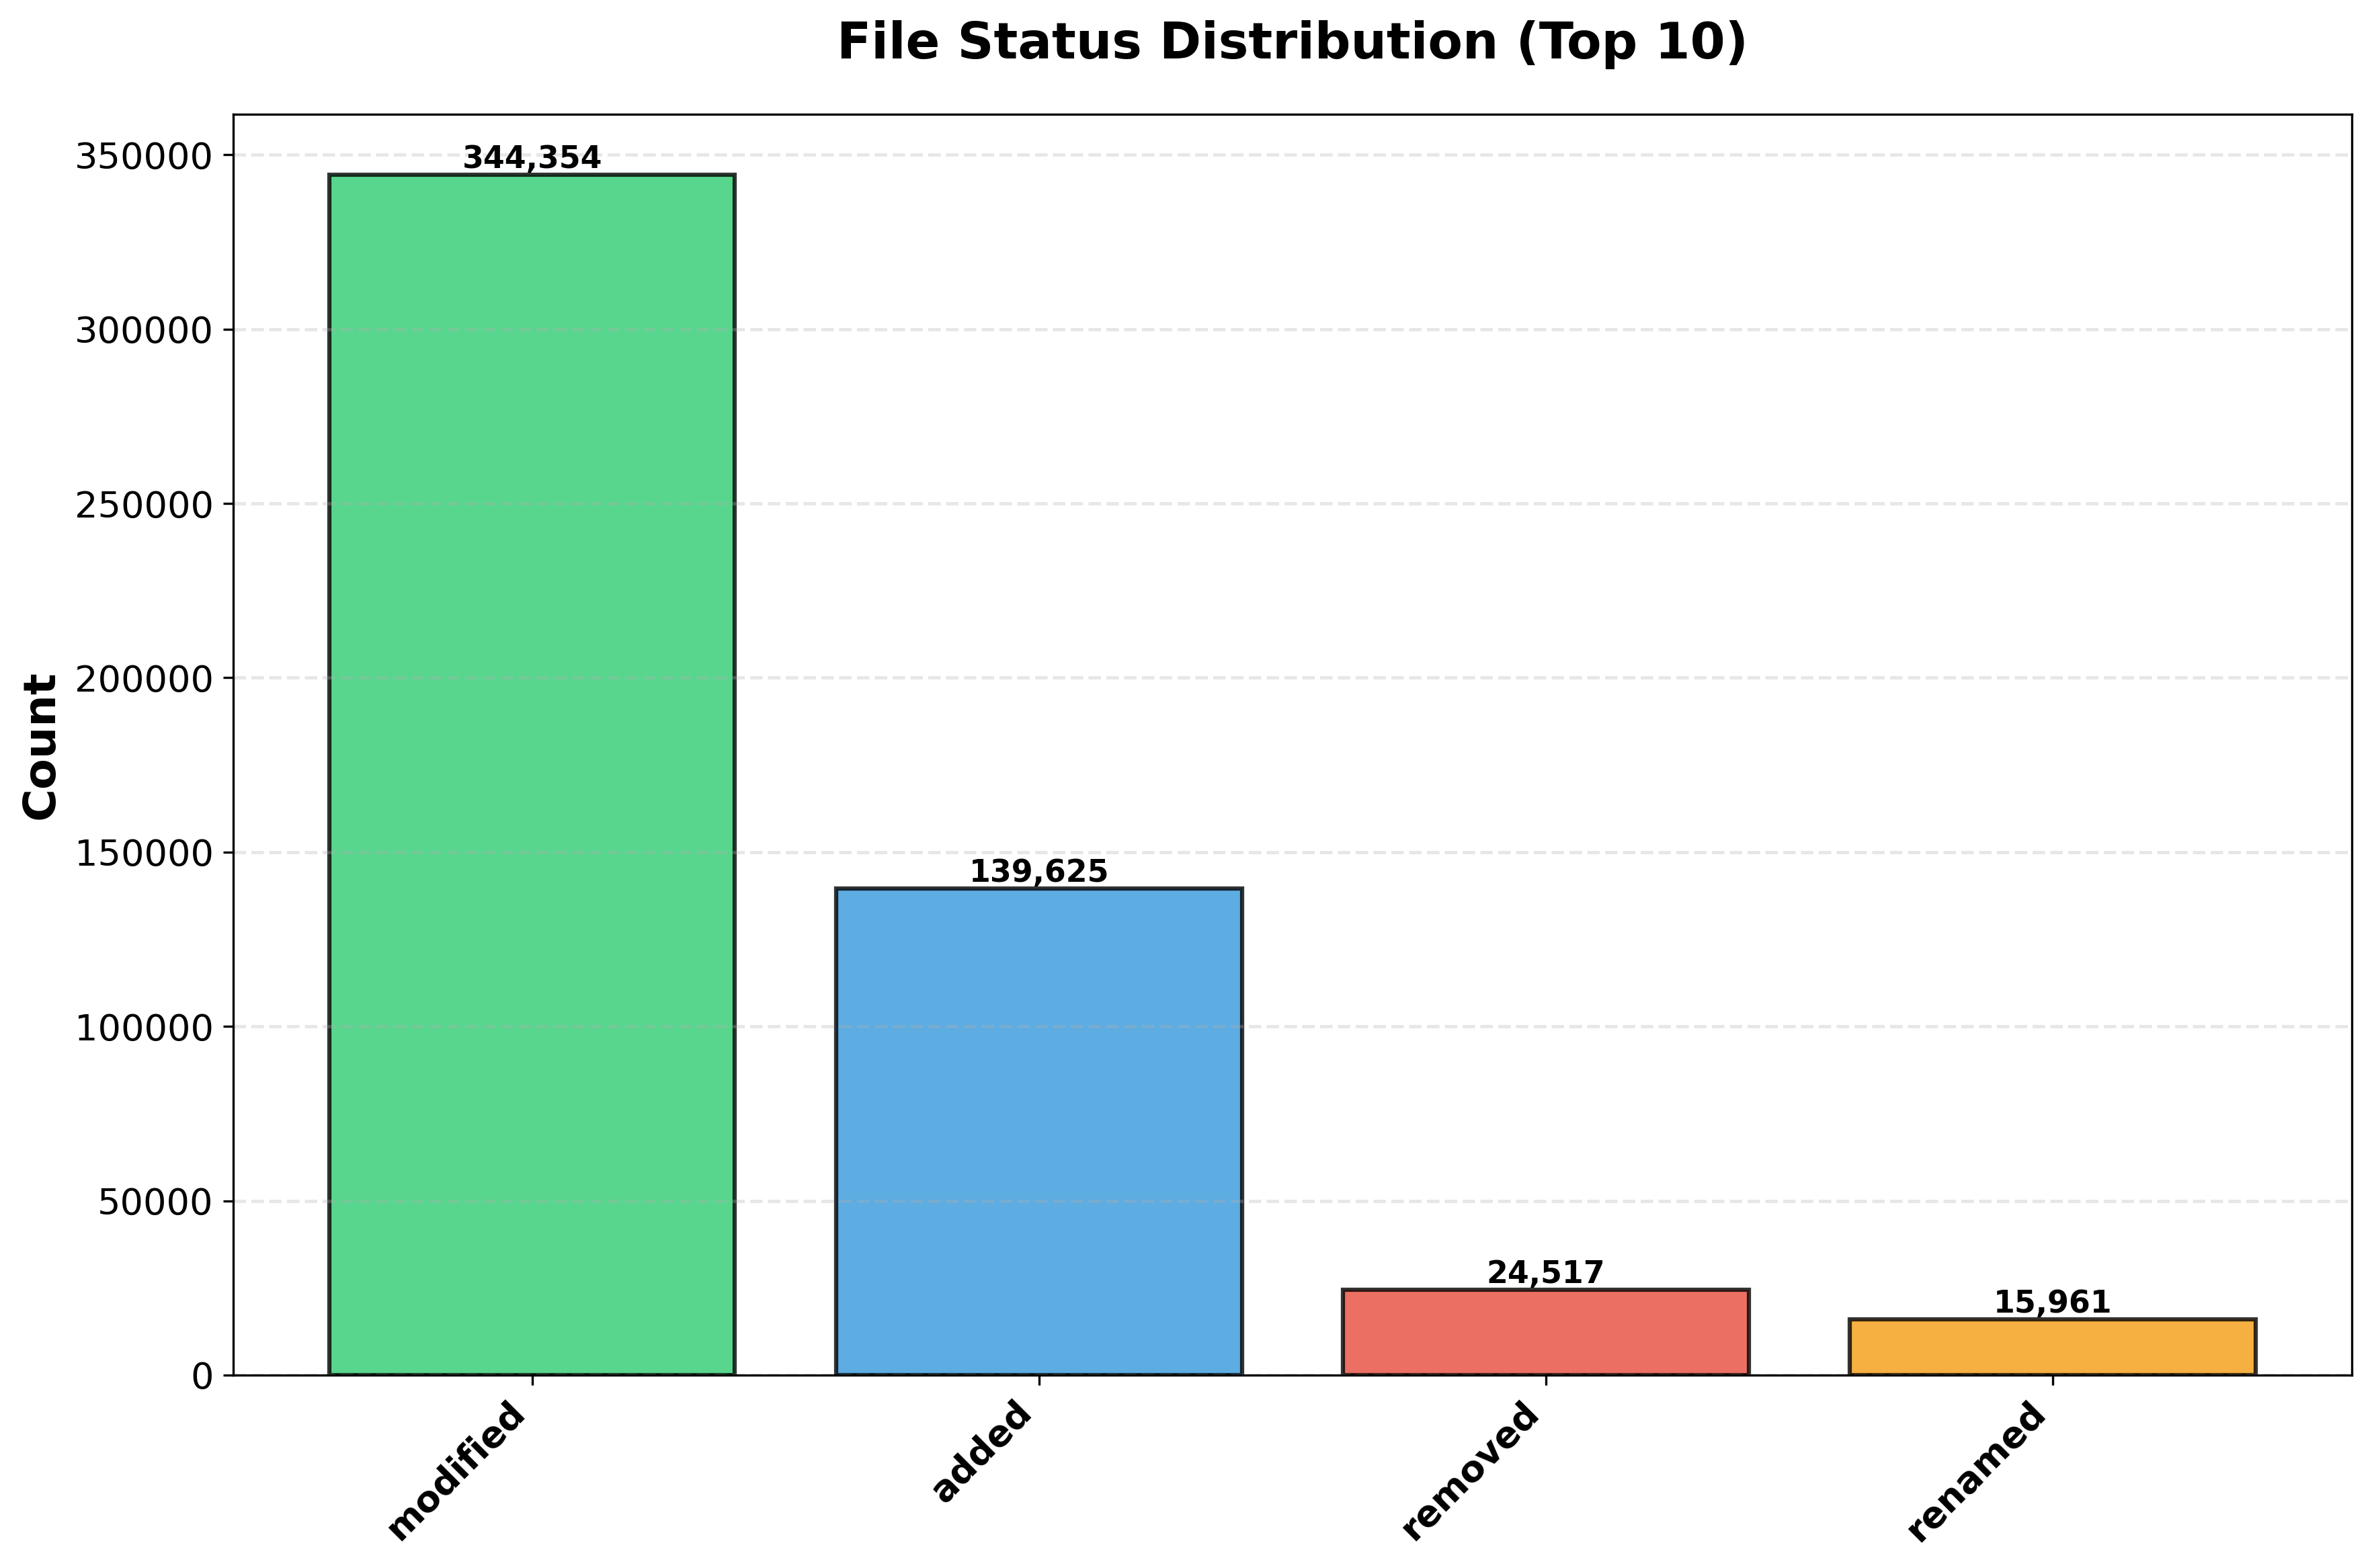
\includegraphics[width=\textwidth]{figures_individual/27_file_status_distribution.png}
\caption{File status distribution}
\label{fig:file_status}
\end{subfigure}
\hfill
\begin{subfigure}[b]{0.48\textwidth}
\centering
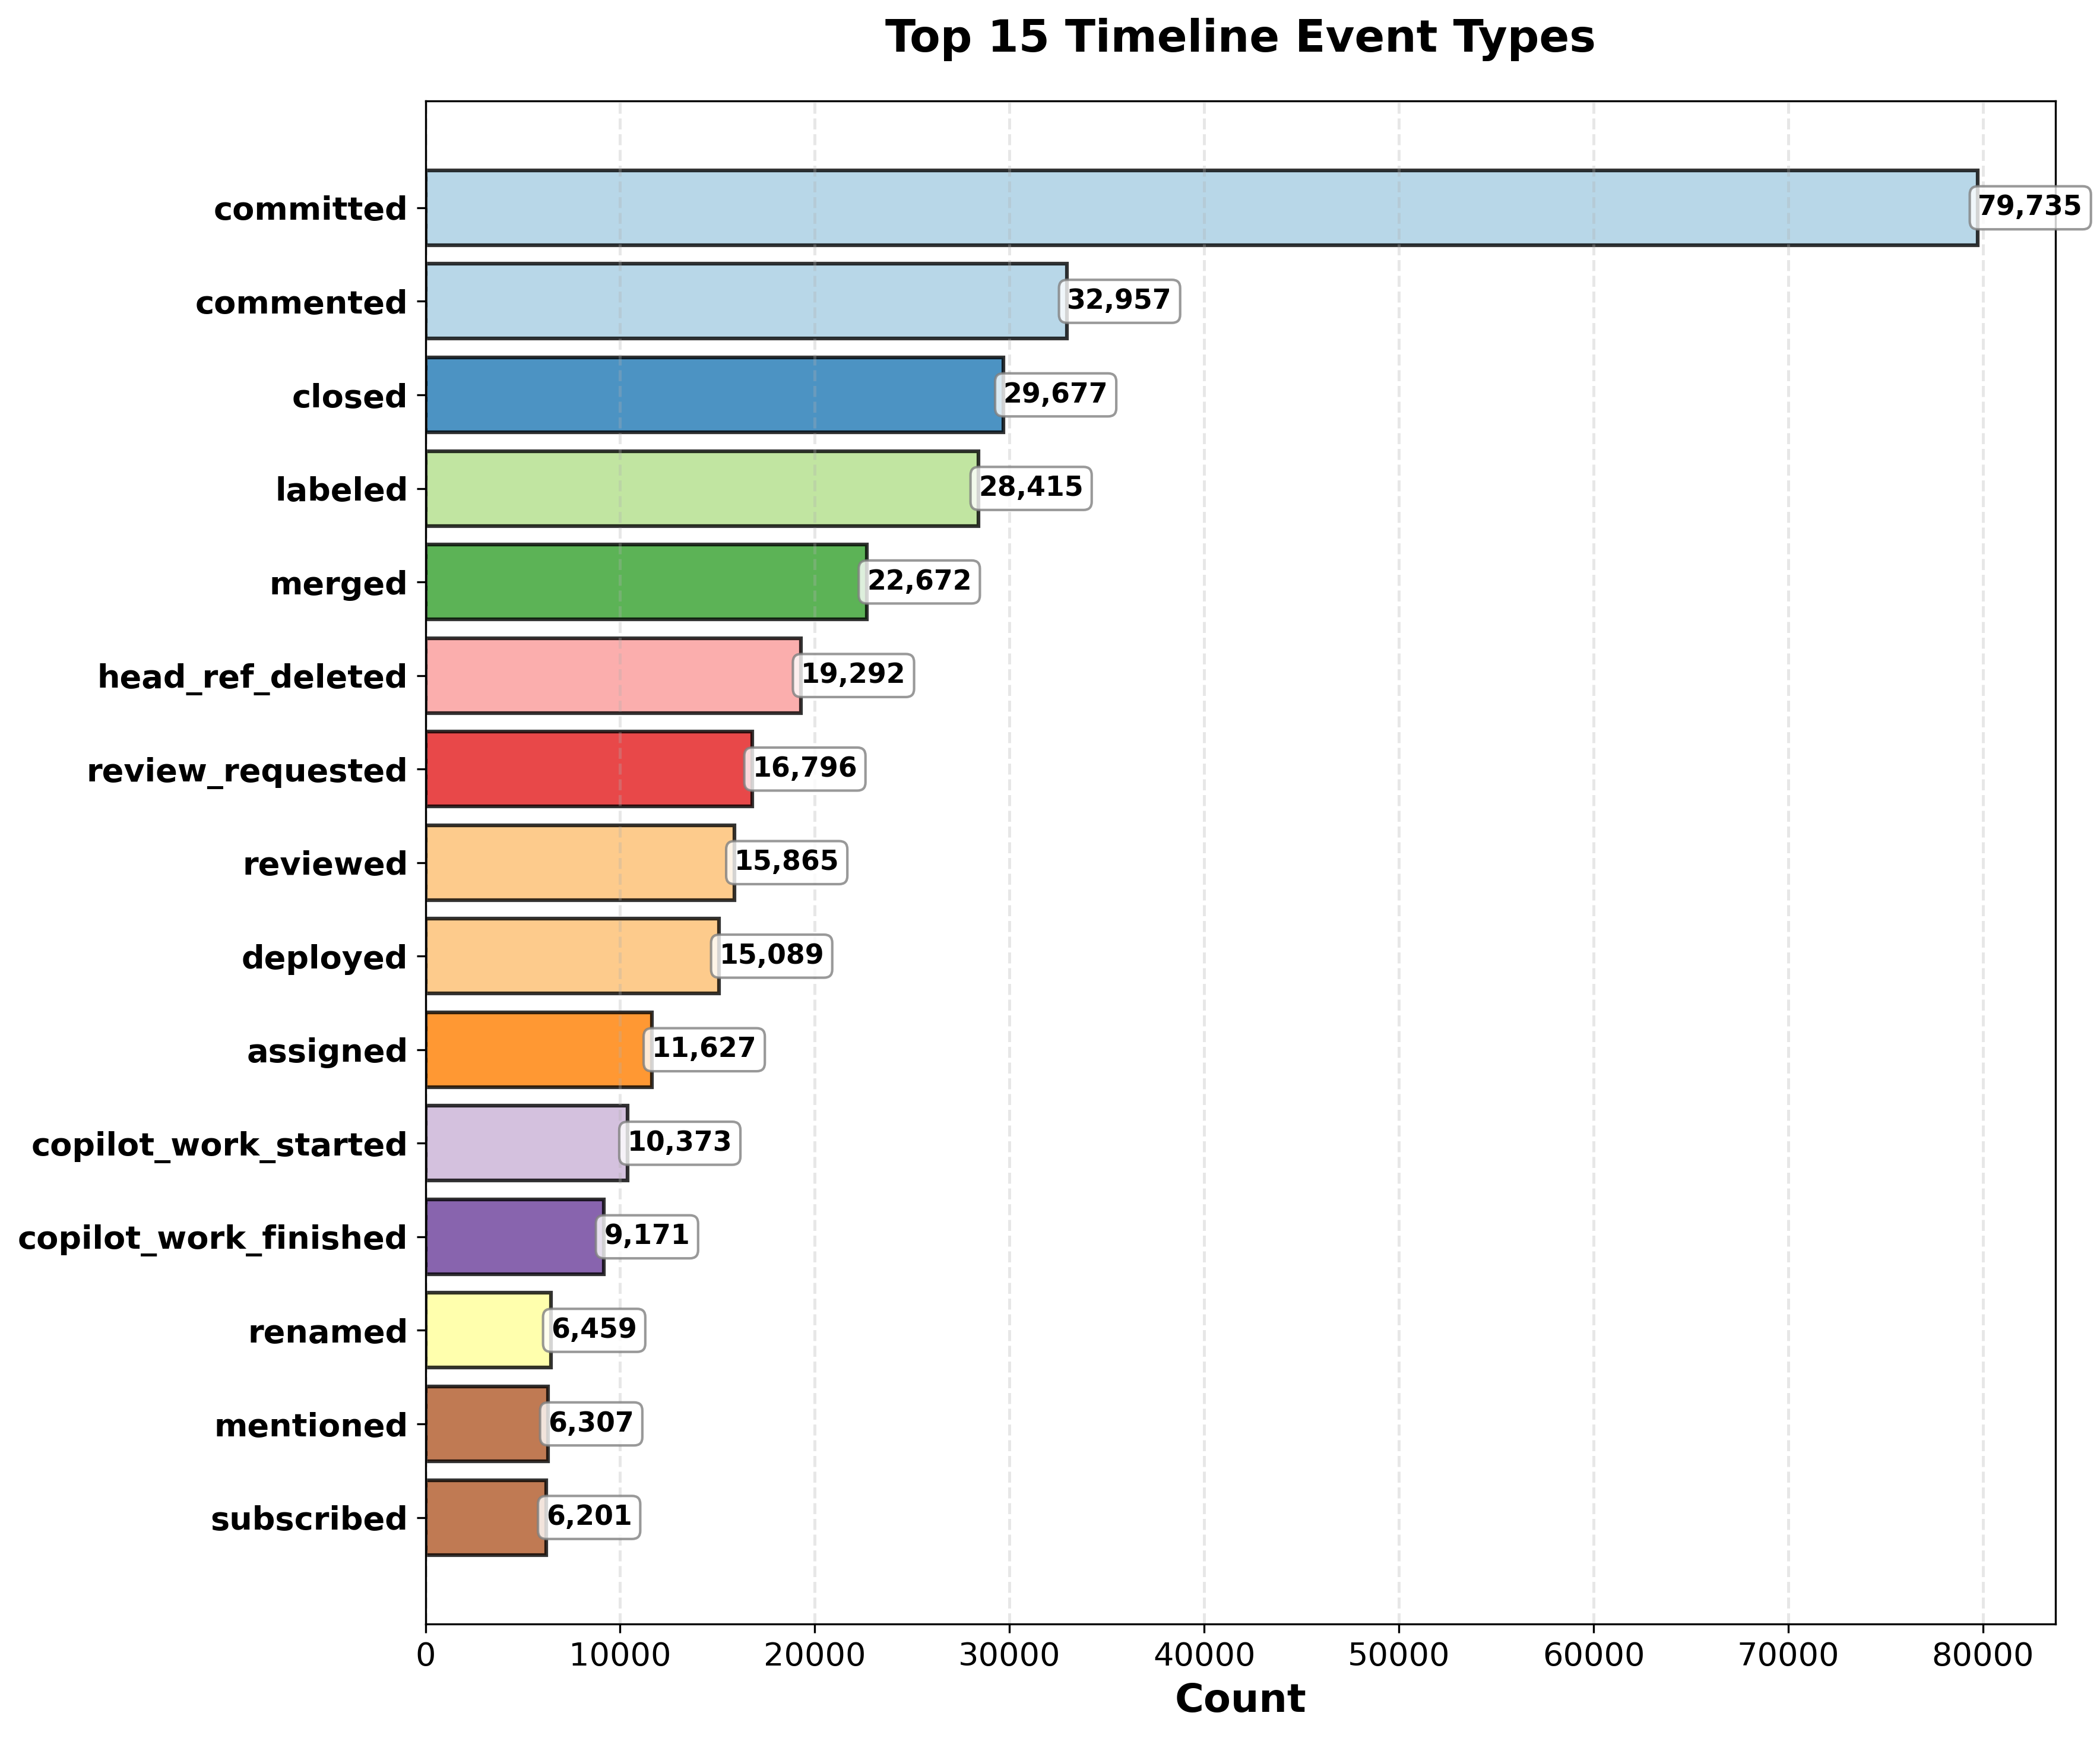
\includegraphics[width=\textwidth]{figures_individual/30_timeline_event_types_barplot.png}
\caption{Top 15 timeline event types}
\label{fig:event_types}
\end{subfigure}

\caption{File-Level Change Distributions (Top events: committed 79K, commented 33K, closed 30K)}
\label{fig:file_level_all}
\end{figure}


\section{Traceability Analysis}

\subsection{Text Blobs, URLs \& Languages}

\begin{table}[H]
\centering
\caption{Text Blob Statistics}
\label{tab:text_blobs}
\begin{tabular}{@{}lrr@{}}
\toprule
\textbf{Entity Type} & \textbf{Count} & \textbf{Avg Length (chars)} \\
\midrule
PR Titles & 33,596 & 42.85 \\
PR Bodies & 33,596 & 930.84 \\
Commit Messages & 88,576 & 79.8 \\
PR Comments & 39,122 & 1,604.62 \\
PR Reviews & 28,875 & 584.30 \\
Issue Bodies & 4,614 & 1,534.7 \\
\midrule
\textbf{Total Text Blobs} & \textbf{228,379} & \textbf{-} \\
\textbf{Non-empty Blobs} & \textbf{206,959} & \textbf{(90.6\%)} \\
\bottomrule
\end{tabular}
\end{table}

\begin{table}[H]
\centering
\caption{URL Analysis and Top Domains}
\small
\begin{tabular}{@{}lrlr@{}}
\toprule
\textbf{Metric} & \textbf{Value} & \textbf{Top Domain} & \textbf{Count (\%)} \\
\midrule
Total URLs & 157,480 & github.com & 24,635 (15.64\%) \\
Unique URLs & 84,451 & chatgpt.com & 17,417 (11.06\%) \\
URLs/Blob (avg) & 0.690 & gh.io & 8,962 (5.69\%) \\
GitHub URLs (internal) & 29,924 (19\%) & vercel.com & 6,775 (4.30\%) \\
External URLs & 127,556 (81\%) & docs.coderabbit.ai & 6,252 (3.97\%) \\
 &  & coderabbit.ai & 5,945 (3.78\%) \\
 &  & app.codecov.io & 5,440 (3.45\%) \\
 &  & app.devin.ai & 4,975 (3.16\%) \\
\bottomrule
\end{tabular}
\end{table}

\subsection{Multi-Language Analysis}
\begin{table}[H]
\centering
\caption{Programming Language Distribution in File Changes}
\small
\begin{tabular}{@{}lrr@{}}
\toprule
\textbf{Language} & \textbf{Files} & \textbf{Percentage} \\
\midrule
Other & 338,010 & 47.48\% \\
TypeScript & 112,252 & 15.77\% \\
Markdown & 40,401 & 5.67\% \\
Python & 39,837 & 5.60\% \\
Go & 28,194 & 3.96\% \\
JSON & 26,330 & 3.70\% \\
JavaScript & 22,374 & 3.14\% \\
YAML & 16,735 & 2.35\% \\
Rust & 15,605 & 2.19\% \\
Java & 10,277 & 1.44\% \\
C\# & 8,995 & 1.26\% \\
Ruby & 7,965 & 1.12\% \\
Dart & 6,517 & 0.92\% \\
Kotlin & 5,170 & 0.73\% \\
C & 4,592 & 0.65\% \\
C++ & 4,100 & 0.58\% \\
TOML & 4,015 & 0.56\% \\
PHP & 3,753 & 0.53\% \\
HTML & 3,628 & 0.51\% \\
Swift & 2,676 & 0.38\% \\
\bottomrule
\end{tabular}
\end{table}

\begin{table}[H]
\centering
\caption{Multi-Language PR Statistics and Agent Behavior}
\small
\begin{tabular}{@{}lrlr@{}}
\toprule
\textbf{Metric} & \textbf{Value} & \textbf{Agent} & \textbf{Multi-lang \%} \\
\midrule
Total PRs w/ files & 33,580 & Claude Code & 58.7\% (2.55 avg) \\
Single-language & 14,829 (44.2\%) & Cursor & 49.4\% (1.96 avg) \\
Multi-language & 11,666 (34.7\%) & Devin & 44.4\% (1.96 avg) \\
Avg langs/PR & 1.37 & OpenAI Codex & 39.0\% (1.49 avg) \\
Max langs/PR & 15 & Copilot & 0.0\% (0.00 avg) \\
\midrule
\multicolumn{4}{l}{\textit{Top Language Combos: Go+MD (2,698), MD+Py (737), MD+TS (372)}} \\
\multicolumn{4}{l}{\textit{Natural Languages: English 98.7\%, Chinese 0.5\%, Spanish 0.4\%}} \\
\bottomrule
\end{tabular}
\end{table}

\section{Temporal Evolution}

\begin{figure}[H]
\centering
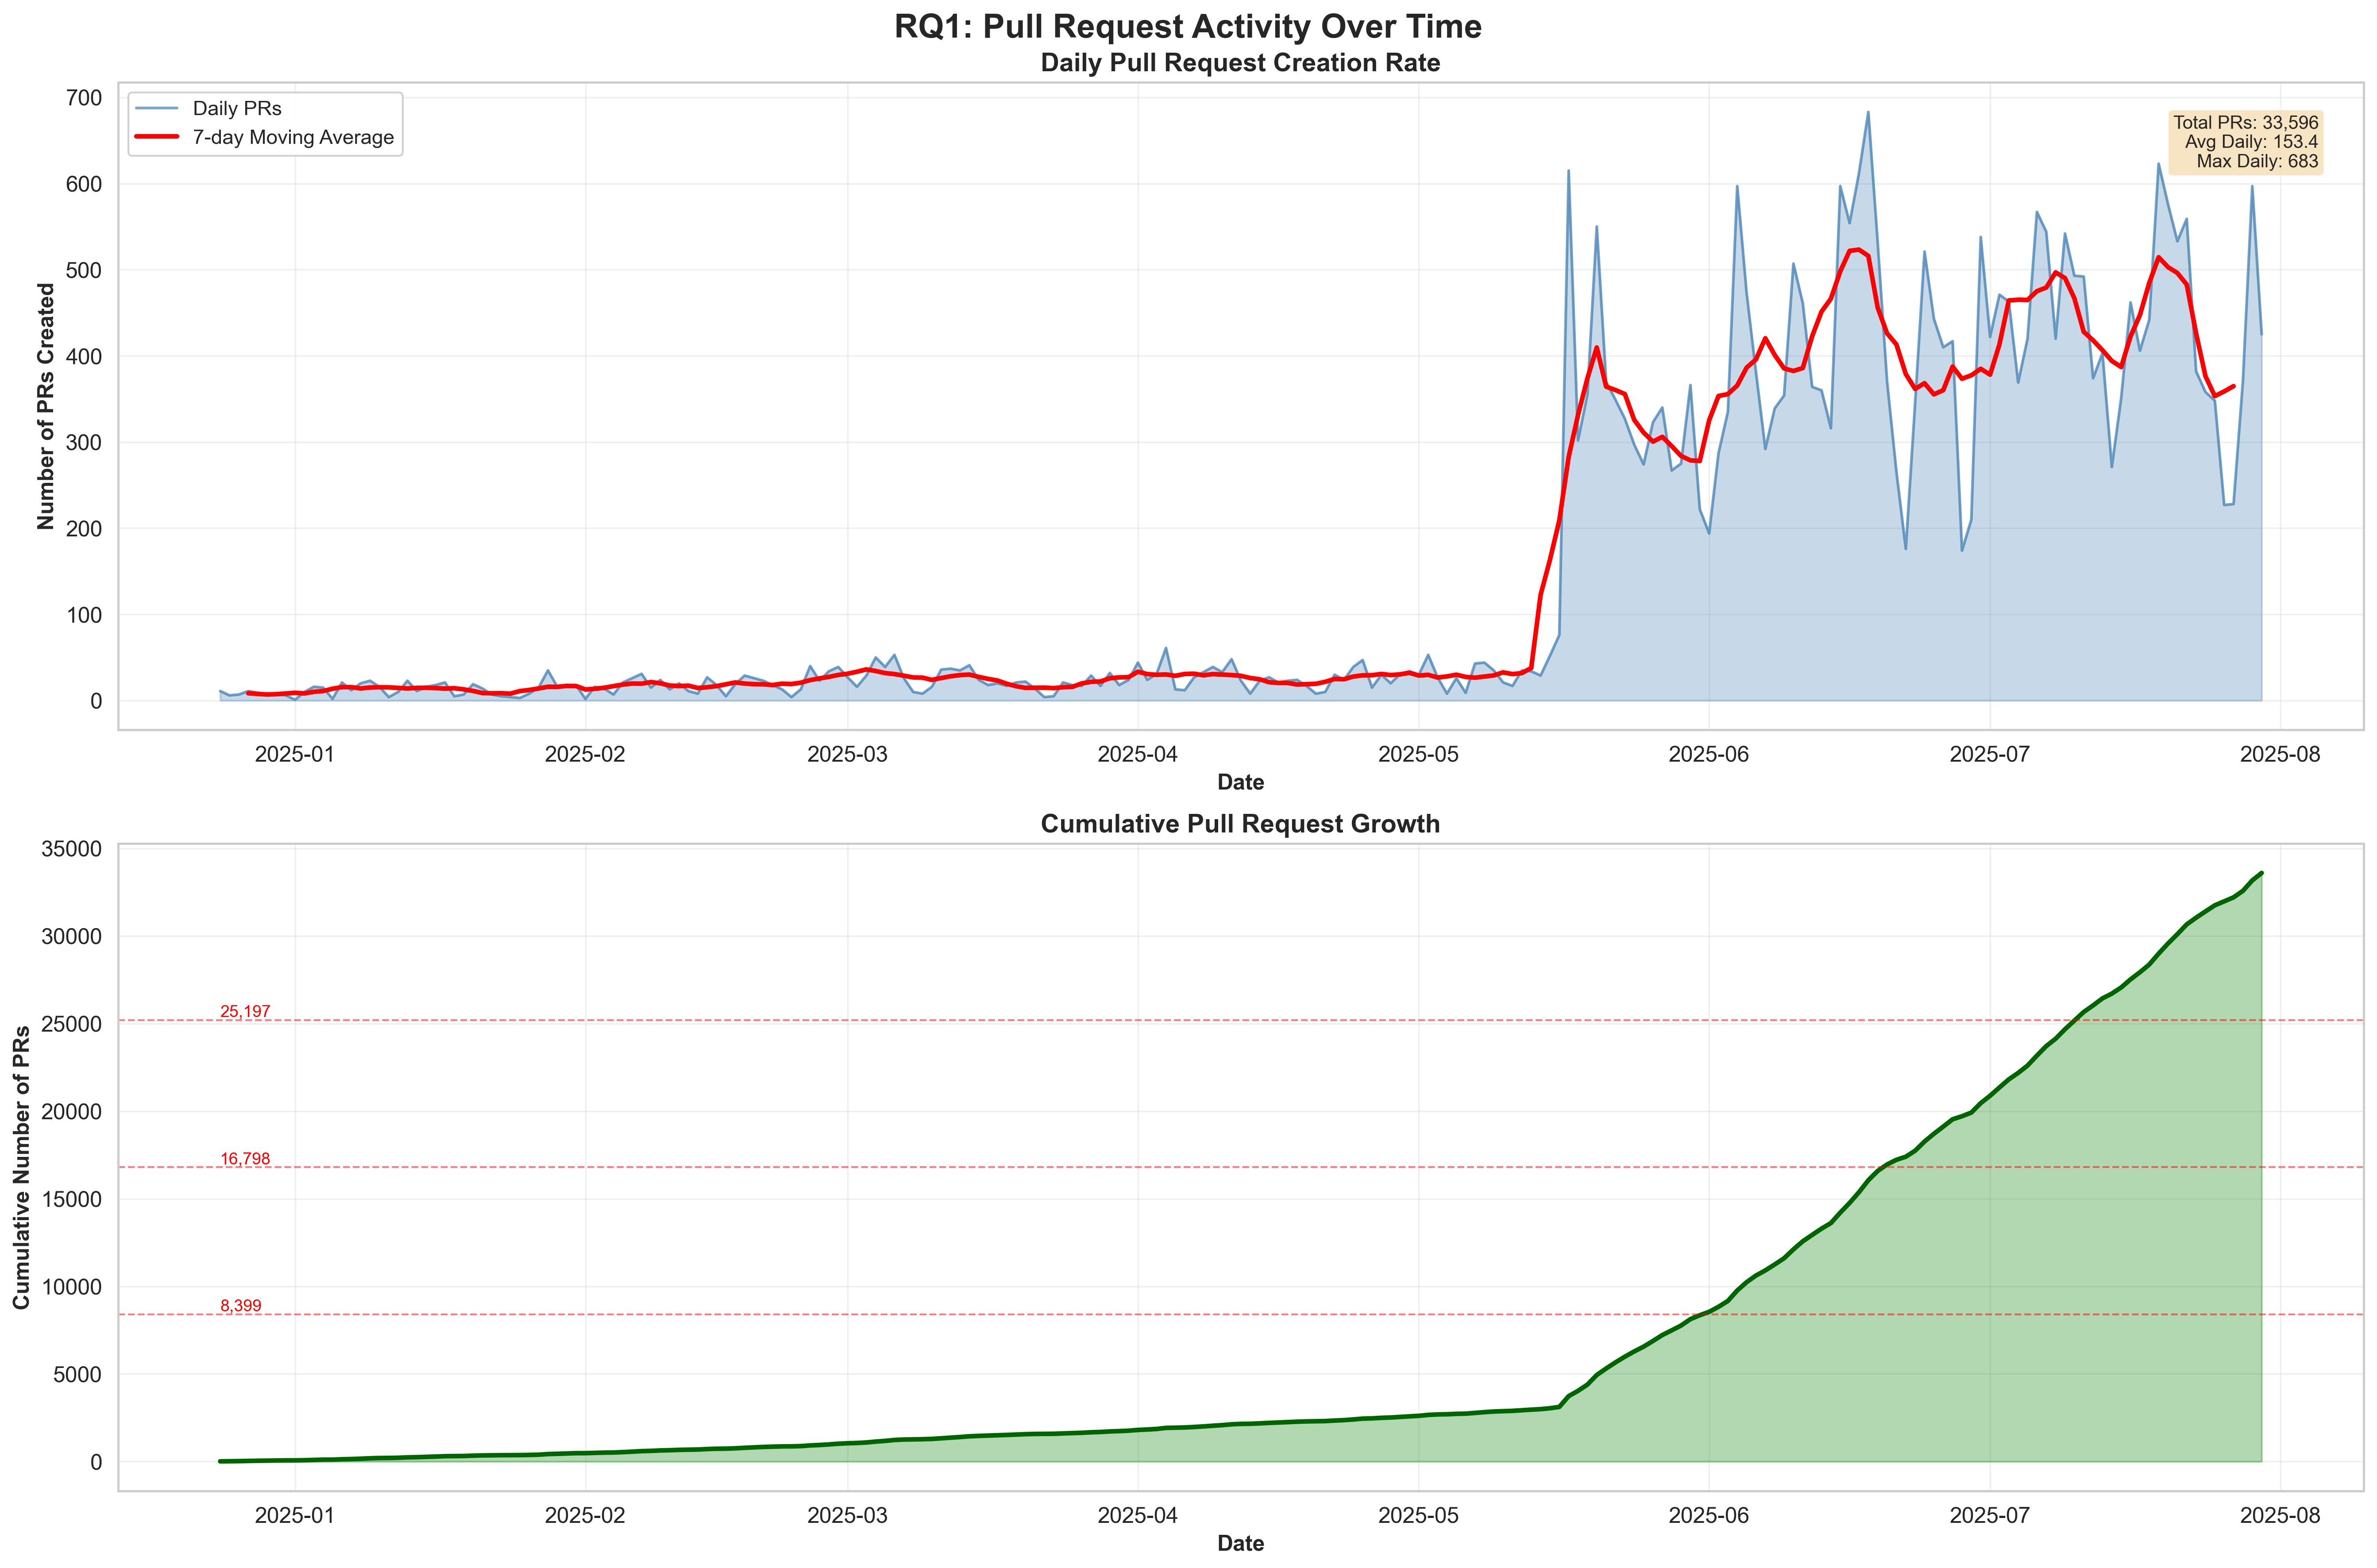
\includegraphics[width=0.95\textwidth]{figures/temporal_01_pr_growth.png}
\caption{Pull Request Activity Over Time: (Top) Daily PR creation rate with 7-day moving average showing activity fluctuations. (Bottom) Cumulative PR growth demonstrating steady dataset expansion over the collection period.}
\label{fig:temporal_pr}
\end{figure}

\begin{figure}[H]
\centering
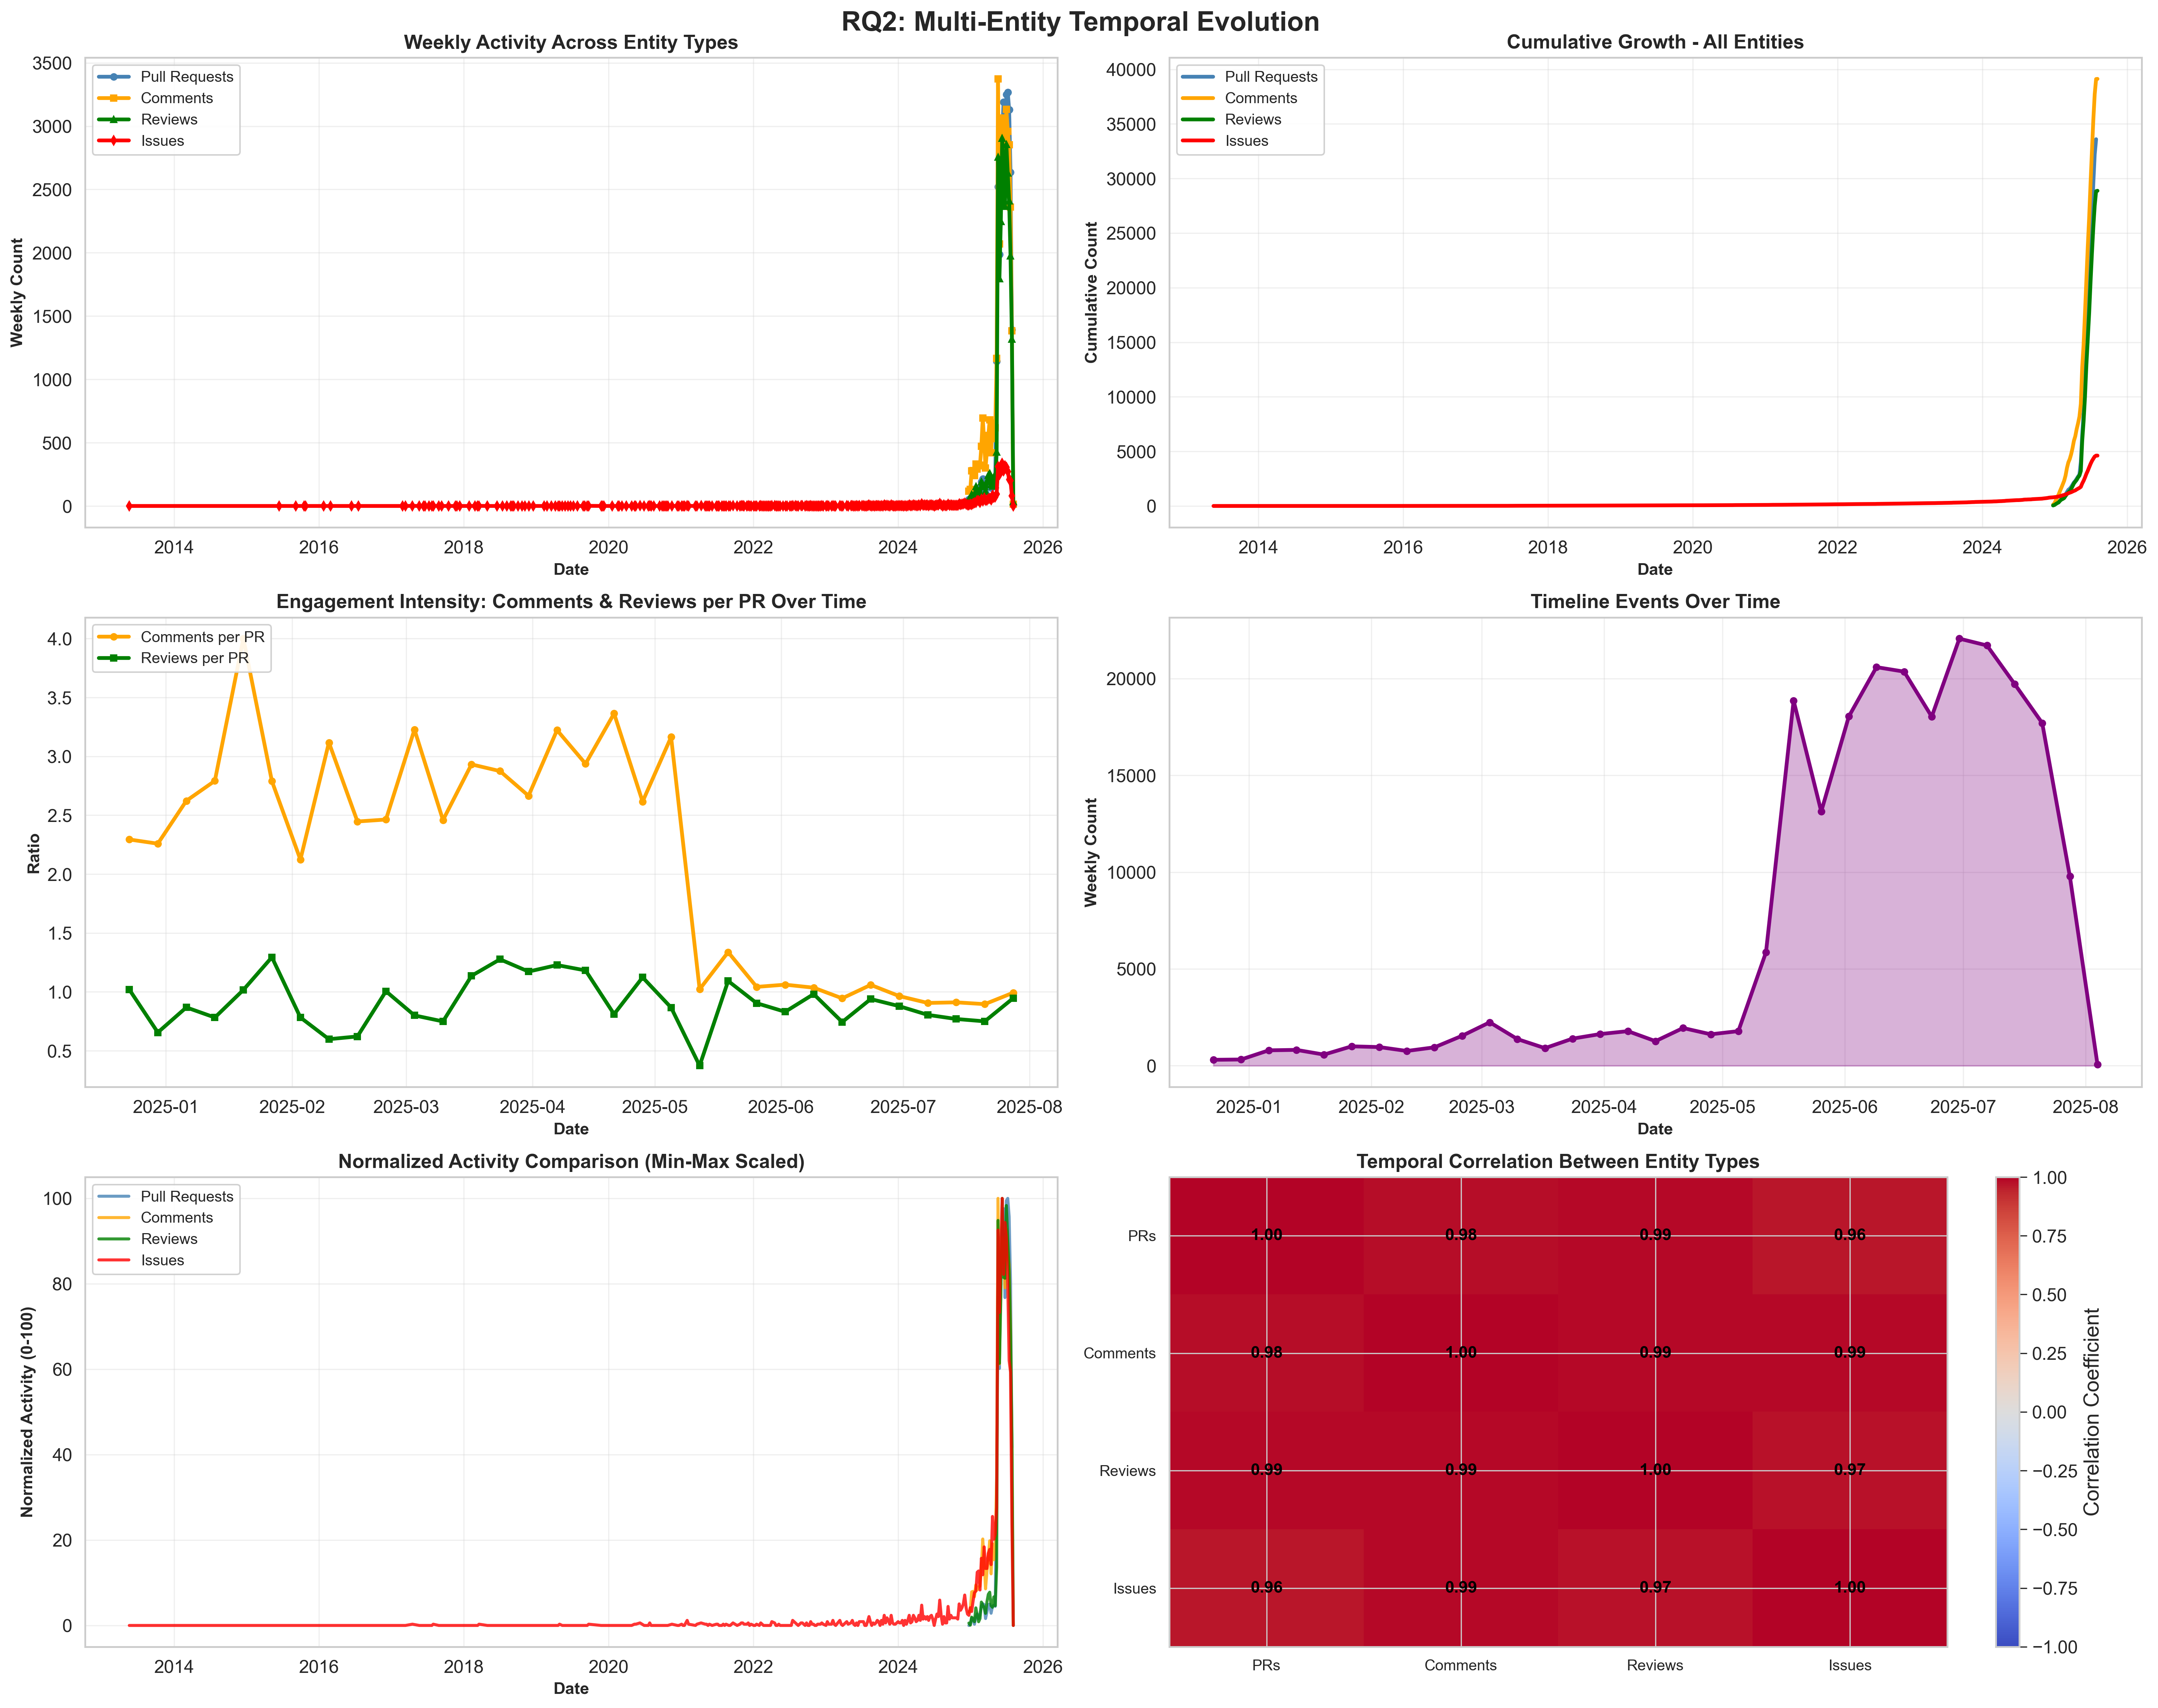
\includegraphics[width=\textwidth]{figures/temporal_02_multi_entity_evolution.png}
\caption{Multi-Entity Temporal Evolution: (Top) Weekly activity and cumulative growth for PRs, comments, reviews, and issues. (Middle) Engagement intensity ratios and timeline events. (Bottom) Normalized comparison and correlation heatmap showing strong positive correlations between entity types (r > 0.7 for most pairs).}
\label{fig:temporal_multi}
\end{figure}

\begin{figure}[H]
\centering
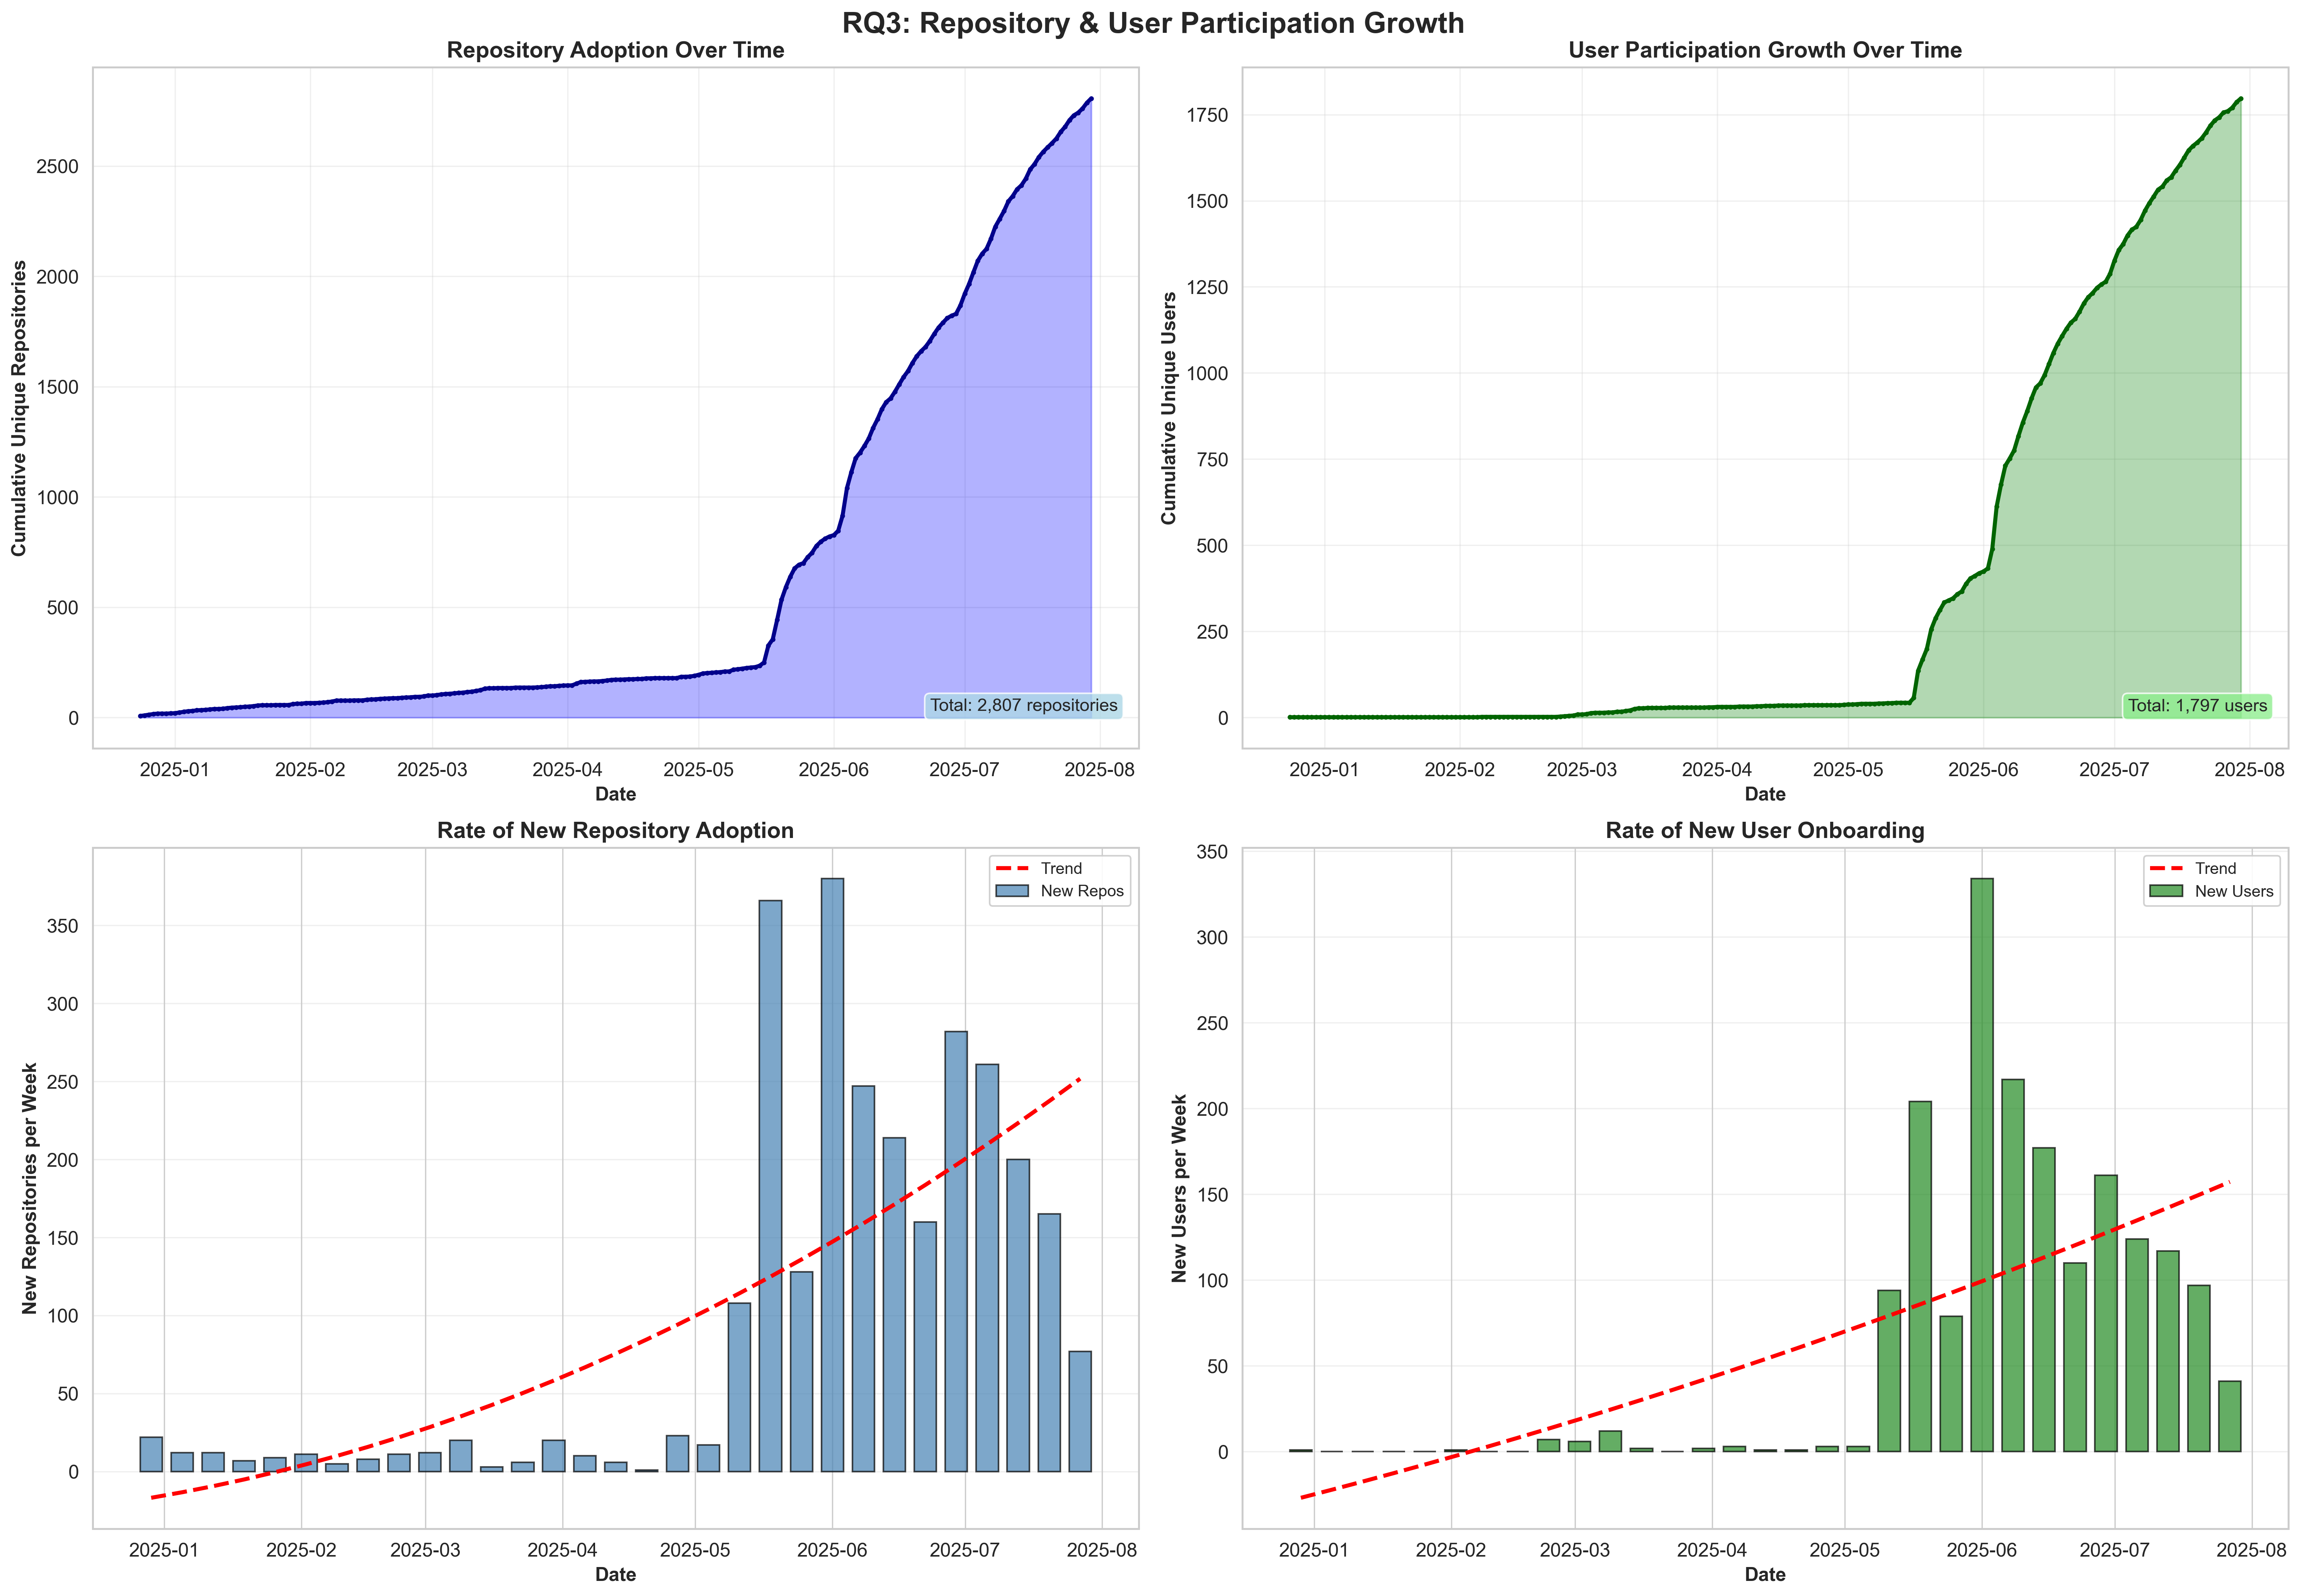
\includegraphics[width=\textwidth]{figures/temporal_03_repo_user_growth.png}
\caption{Repository and User Participation Growth: (Top) Cumulative unique repositories and users over time showing steady growth. (Bottom) Rate of new repository adoption and user onboarding with polynomial trend lines indicating sustained ecosystem expansion.}
\label{fig:temporal_repo_user}
\end{figure}

\begin{figure}[H]
\centering
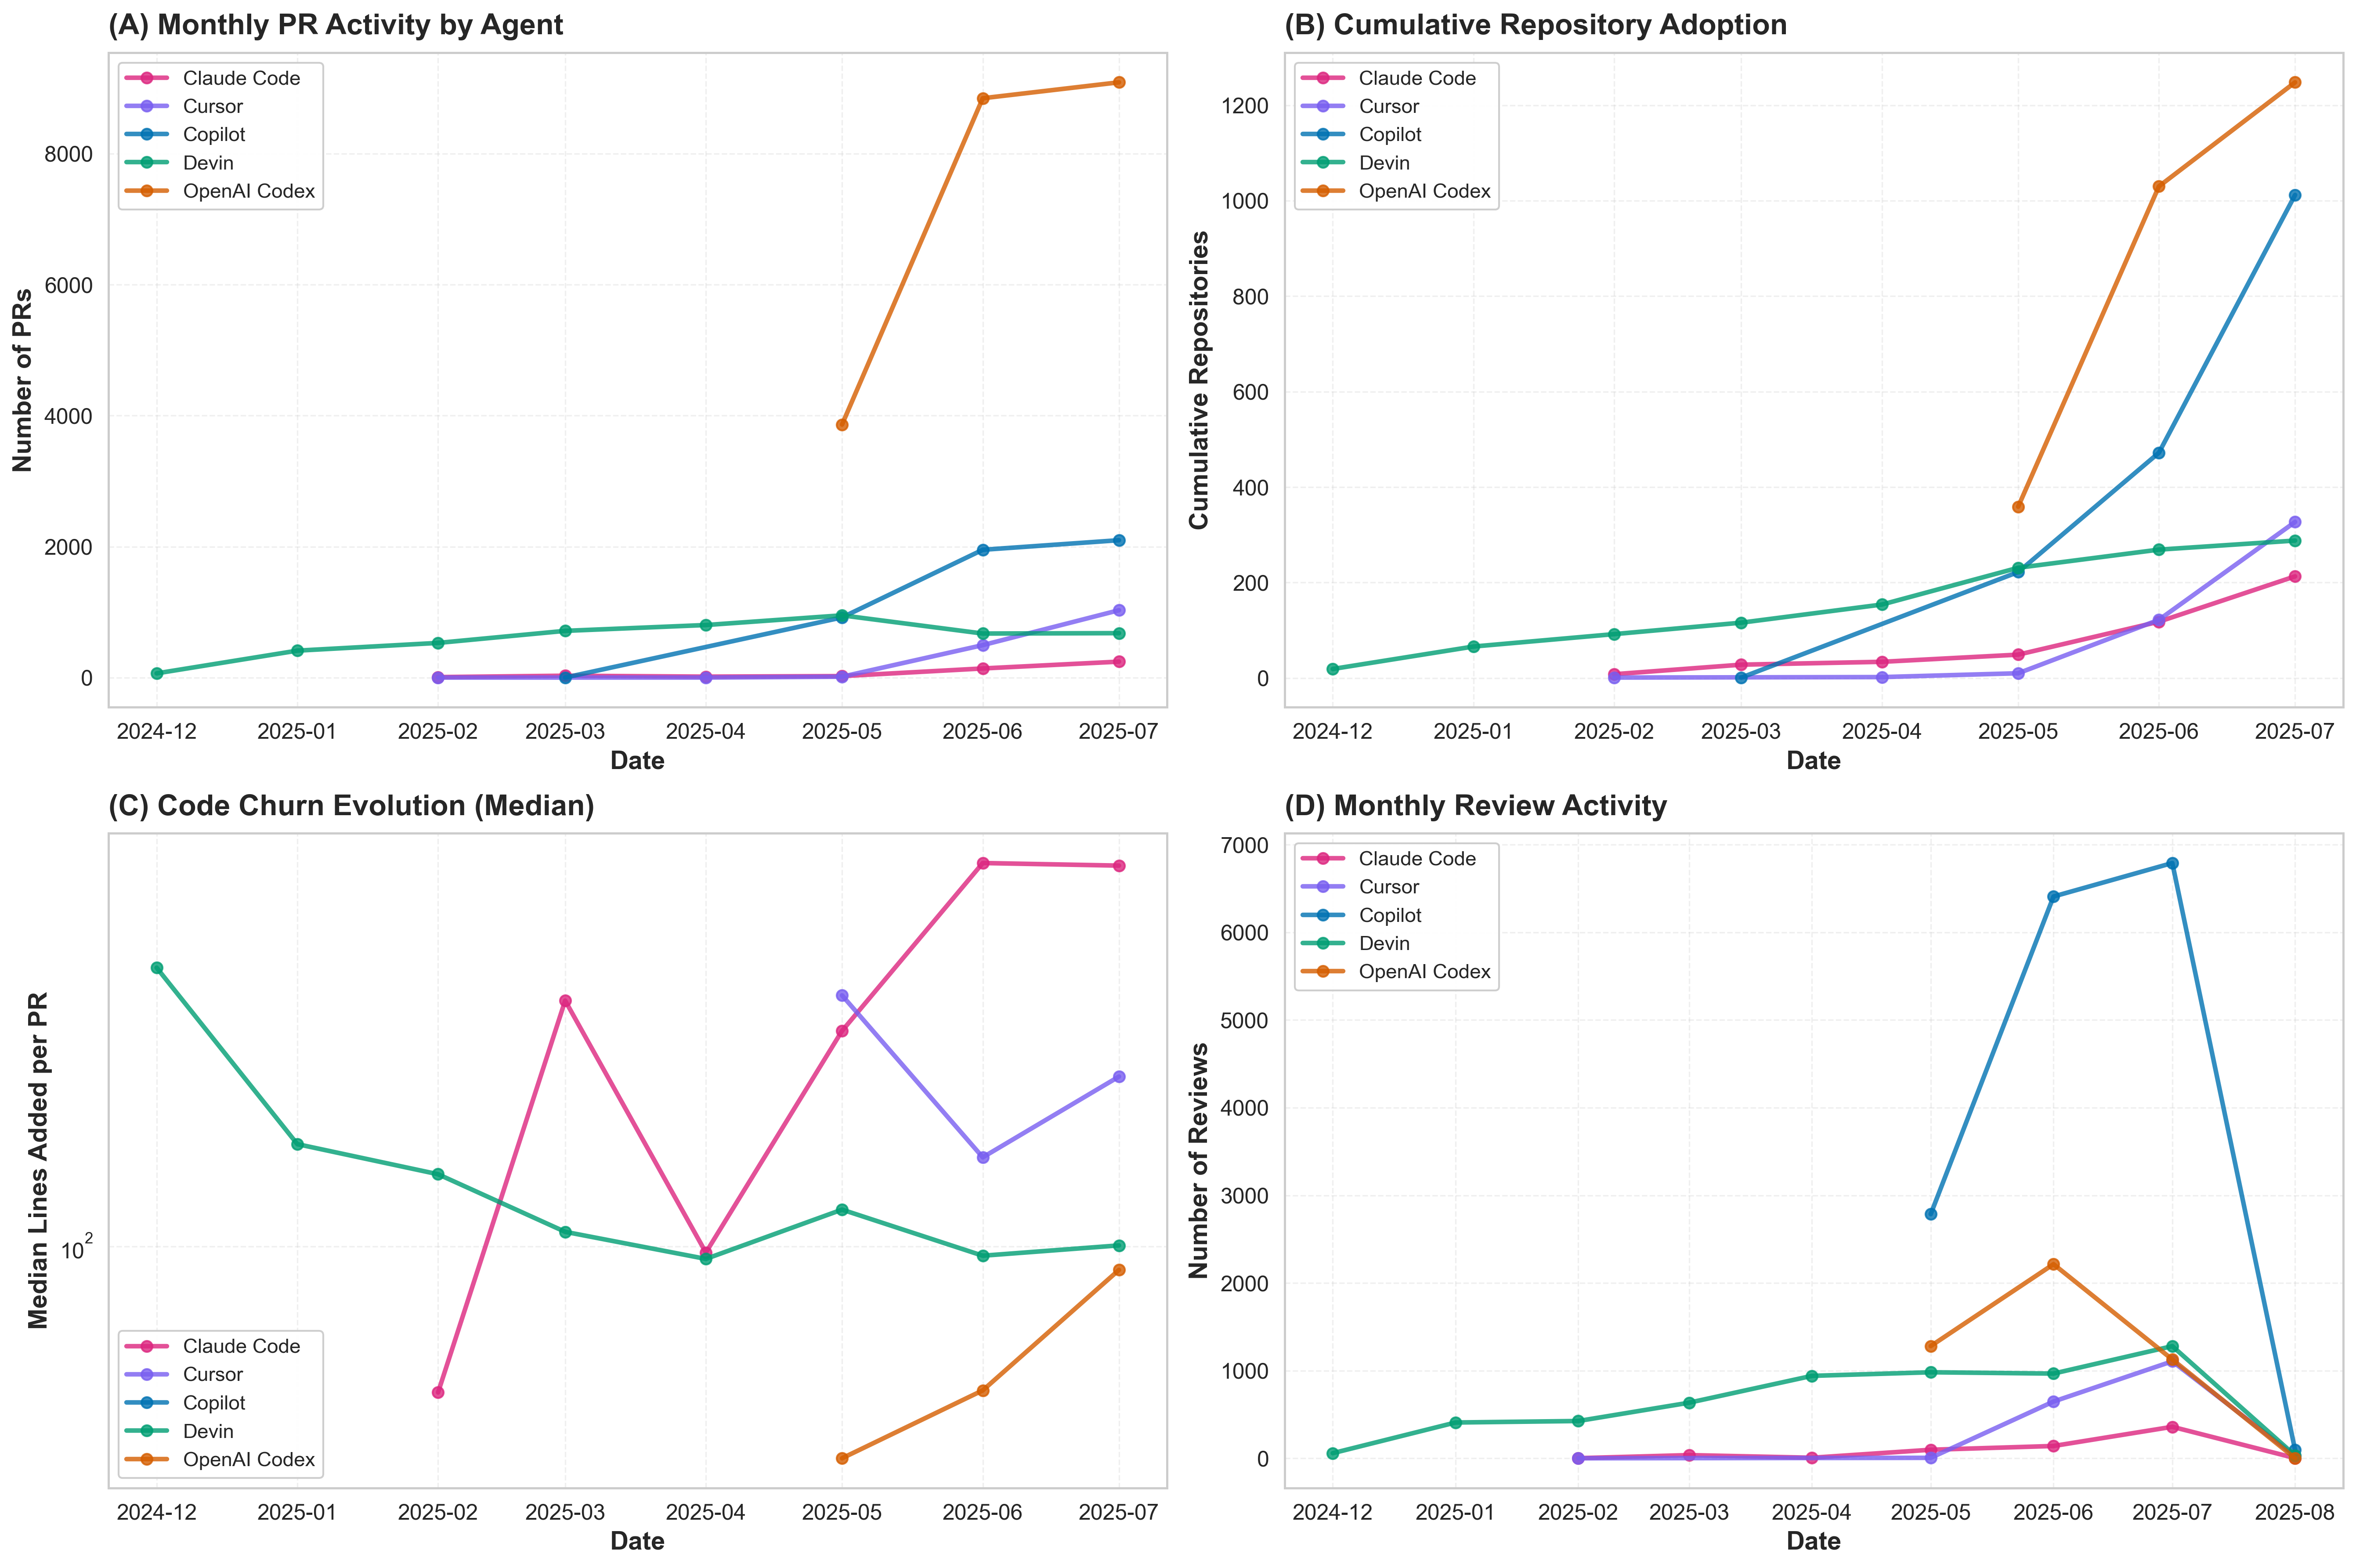
\includegraphics[width=\textwidth]{figures/fig4_temporal_evolution.png}
\caption{Temporal Evolution by Agent: Four-panel time-series analysis showing (Top Left) Monthly PR activity by agent, (Top Right) Cumulative repository adoption, (Bottom Left) Code churn evolution (median lines added), (Bottom Right) Monthly review activity. Reveals distinct growth trajectories and seasonal patterns.}
\label{fig:temporal_evolution}
\end{figure}


\section{Agent-Specific Analysis}

\subsection{Agent Adoption \& Acceptance}

\begin{figure}[H]
\centering
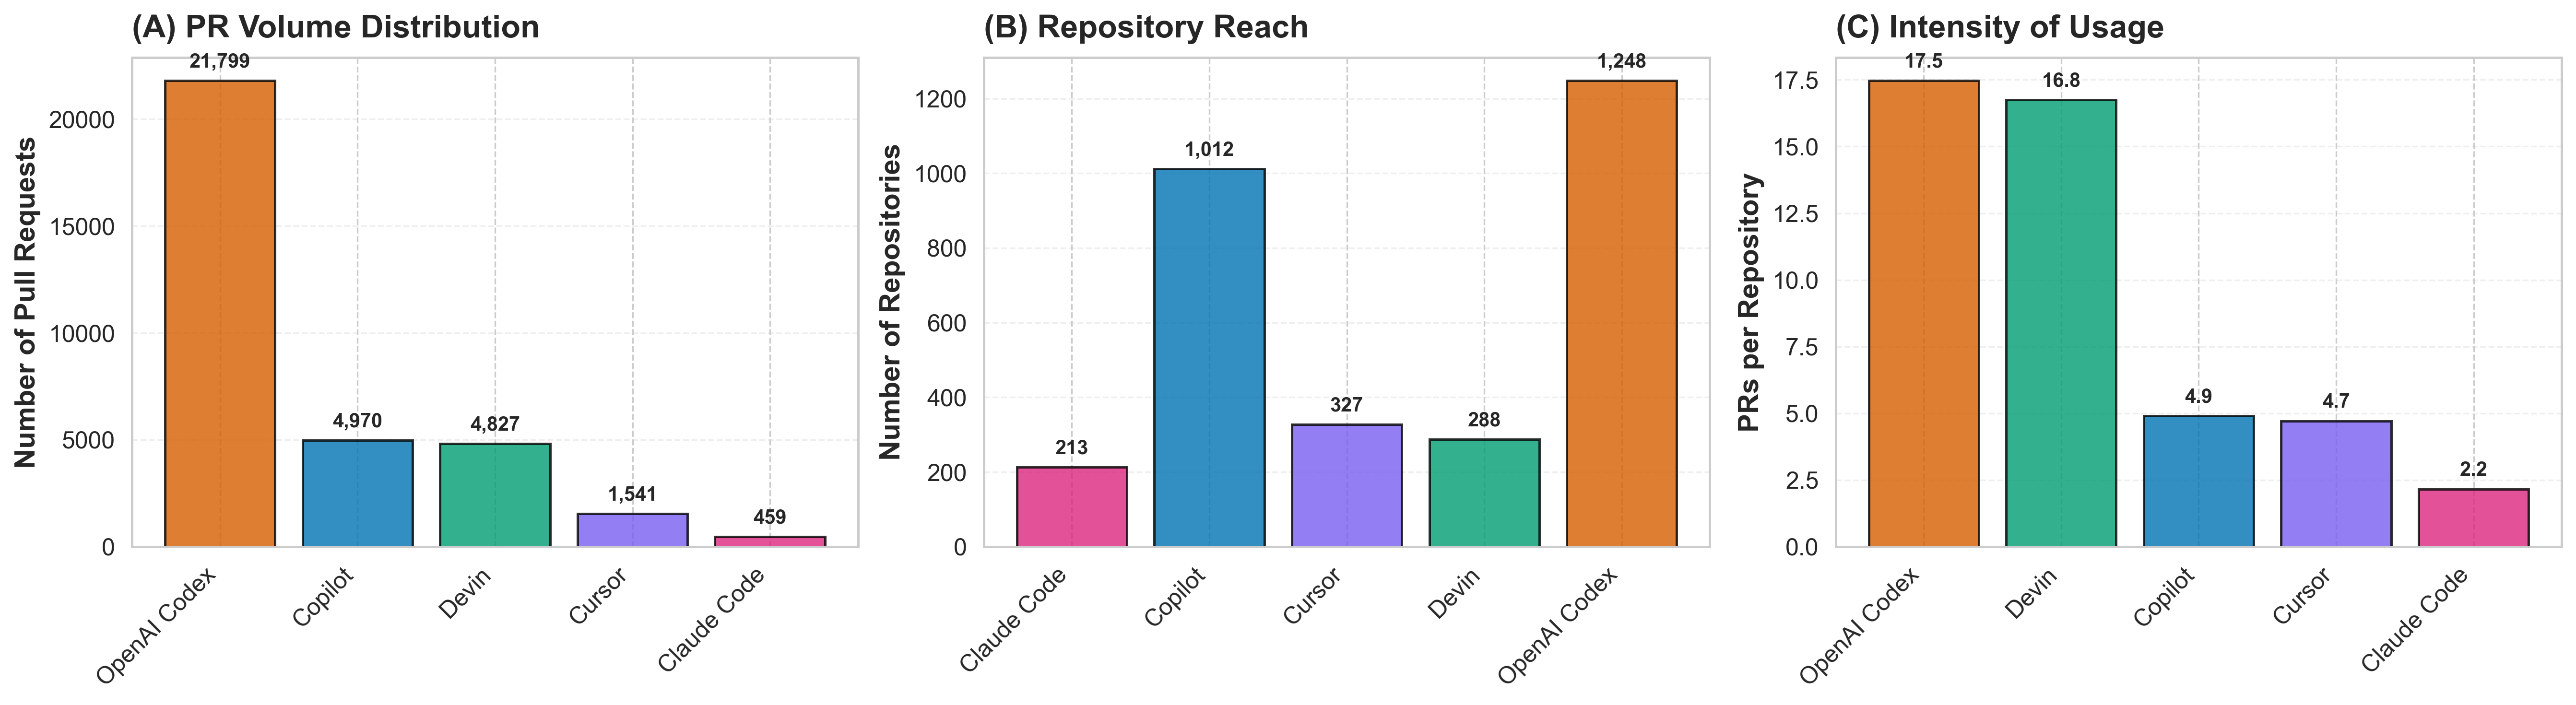
\includegraphics[width=\textwidth]{figures/fig1_agent_adoption_landscape.png}
\caption{Agent Adoption Landscape: (Left) PR volume distribution showing OpenAI Codex dominates with 21,799 PRs (64.89\%). (Middle) Repository reach across agents. (Right) Intensity of usage (PRs per repository) with OpenAI Codex at 17.5 PRs/repo.}
\label{fig:agent_adoption}
\end{figure}

\begin{figure}[H]
\centering
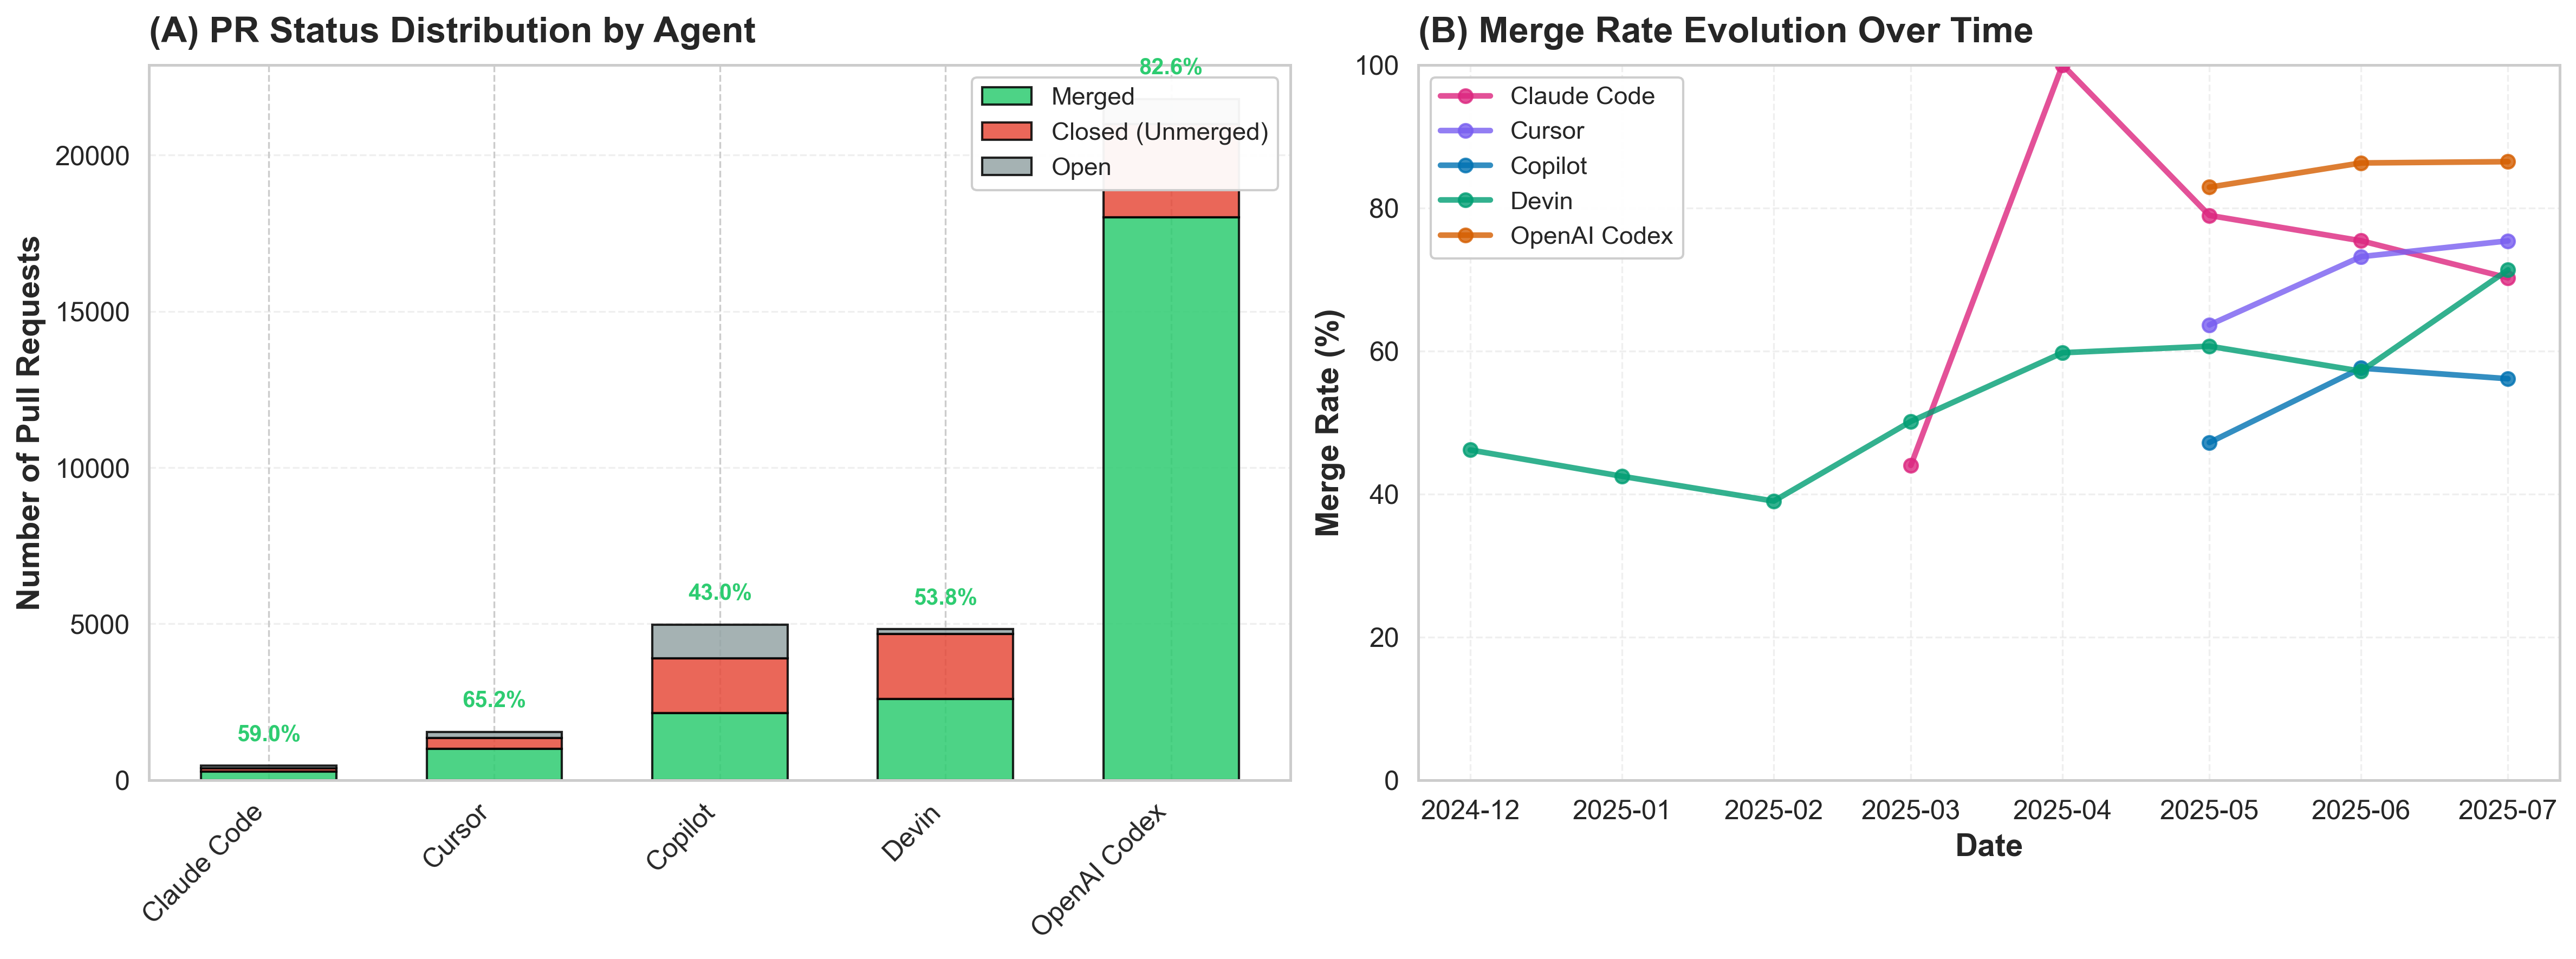
\includegraphics[width=\textwidth]{figures/fig2_pr_acceptance_rates.png}
\caption{PR Acceptance Rates: (Left) PR status distribution by agent showing merge rates from 43\% (Copilot) to 82.6\% (OpenAI Codex). (Right) Temporal trends in merge rates over time, indicating evolving patterns.}
\label{fig:pr_acceptance}
\end{figure}

\subsection{Entity Distributions by Agent}

\begin{figure}[H]
\centering
\begin{subfigure}[b]{0.48\textwidth}
\centering
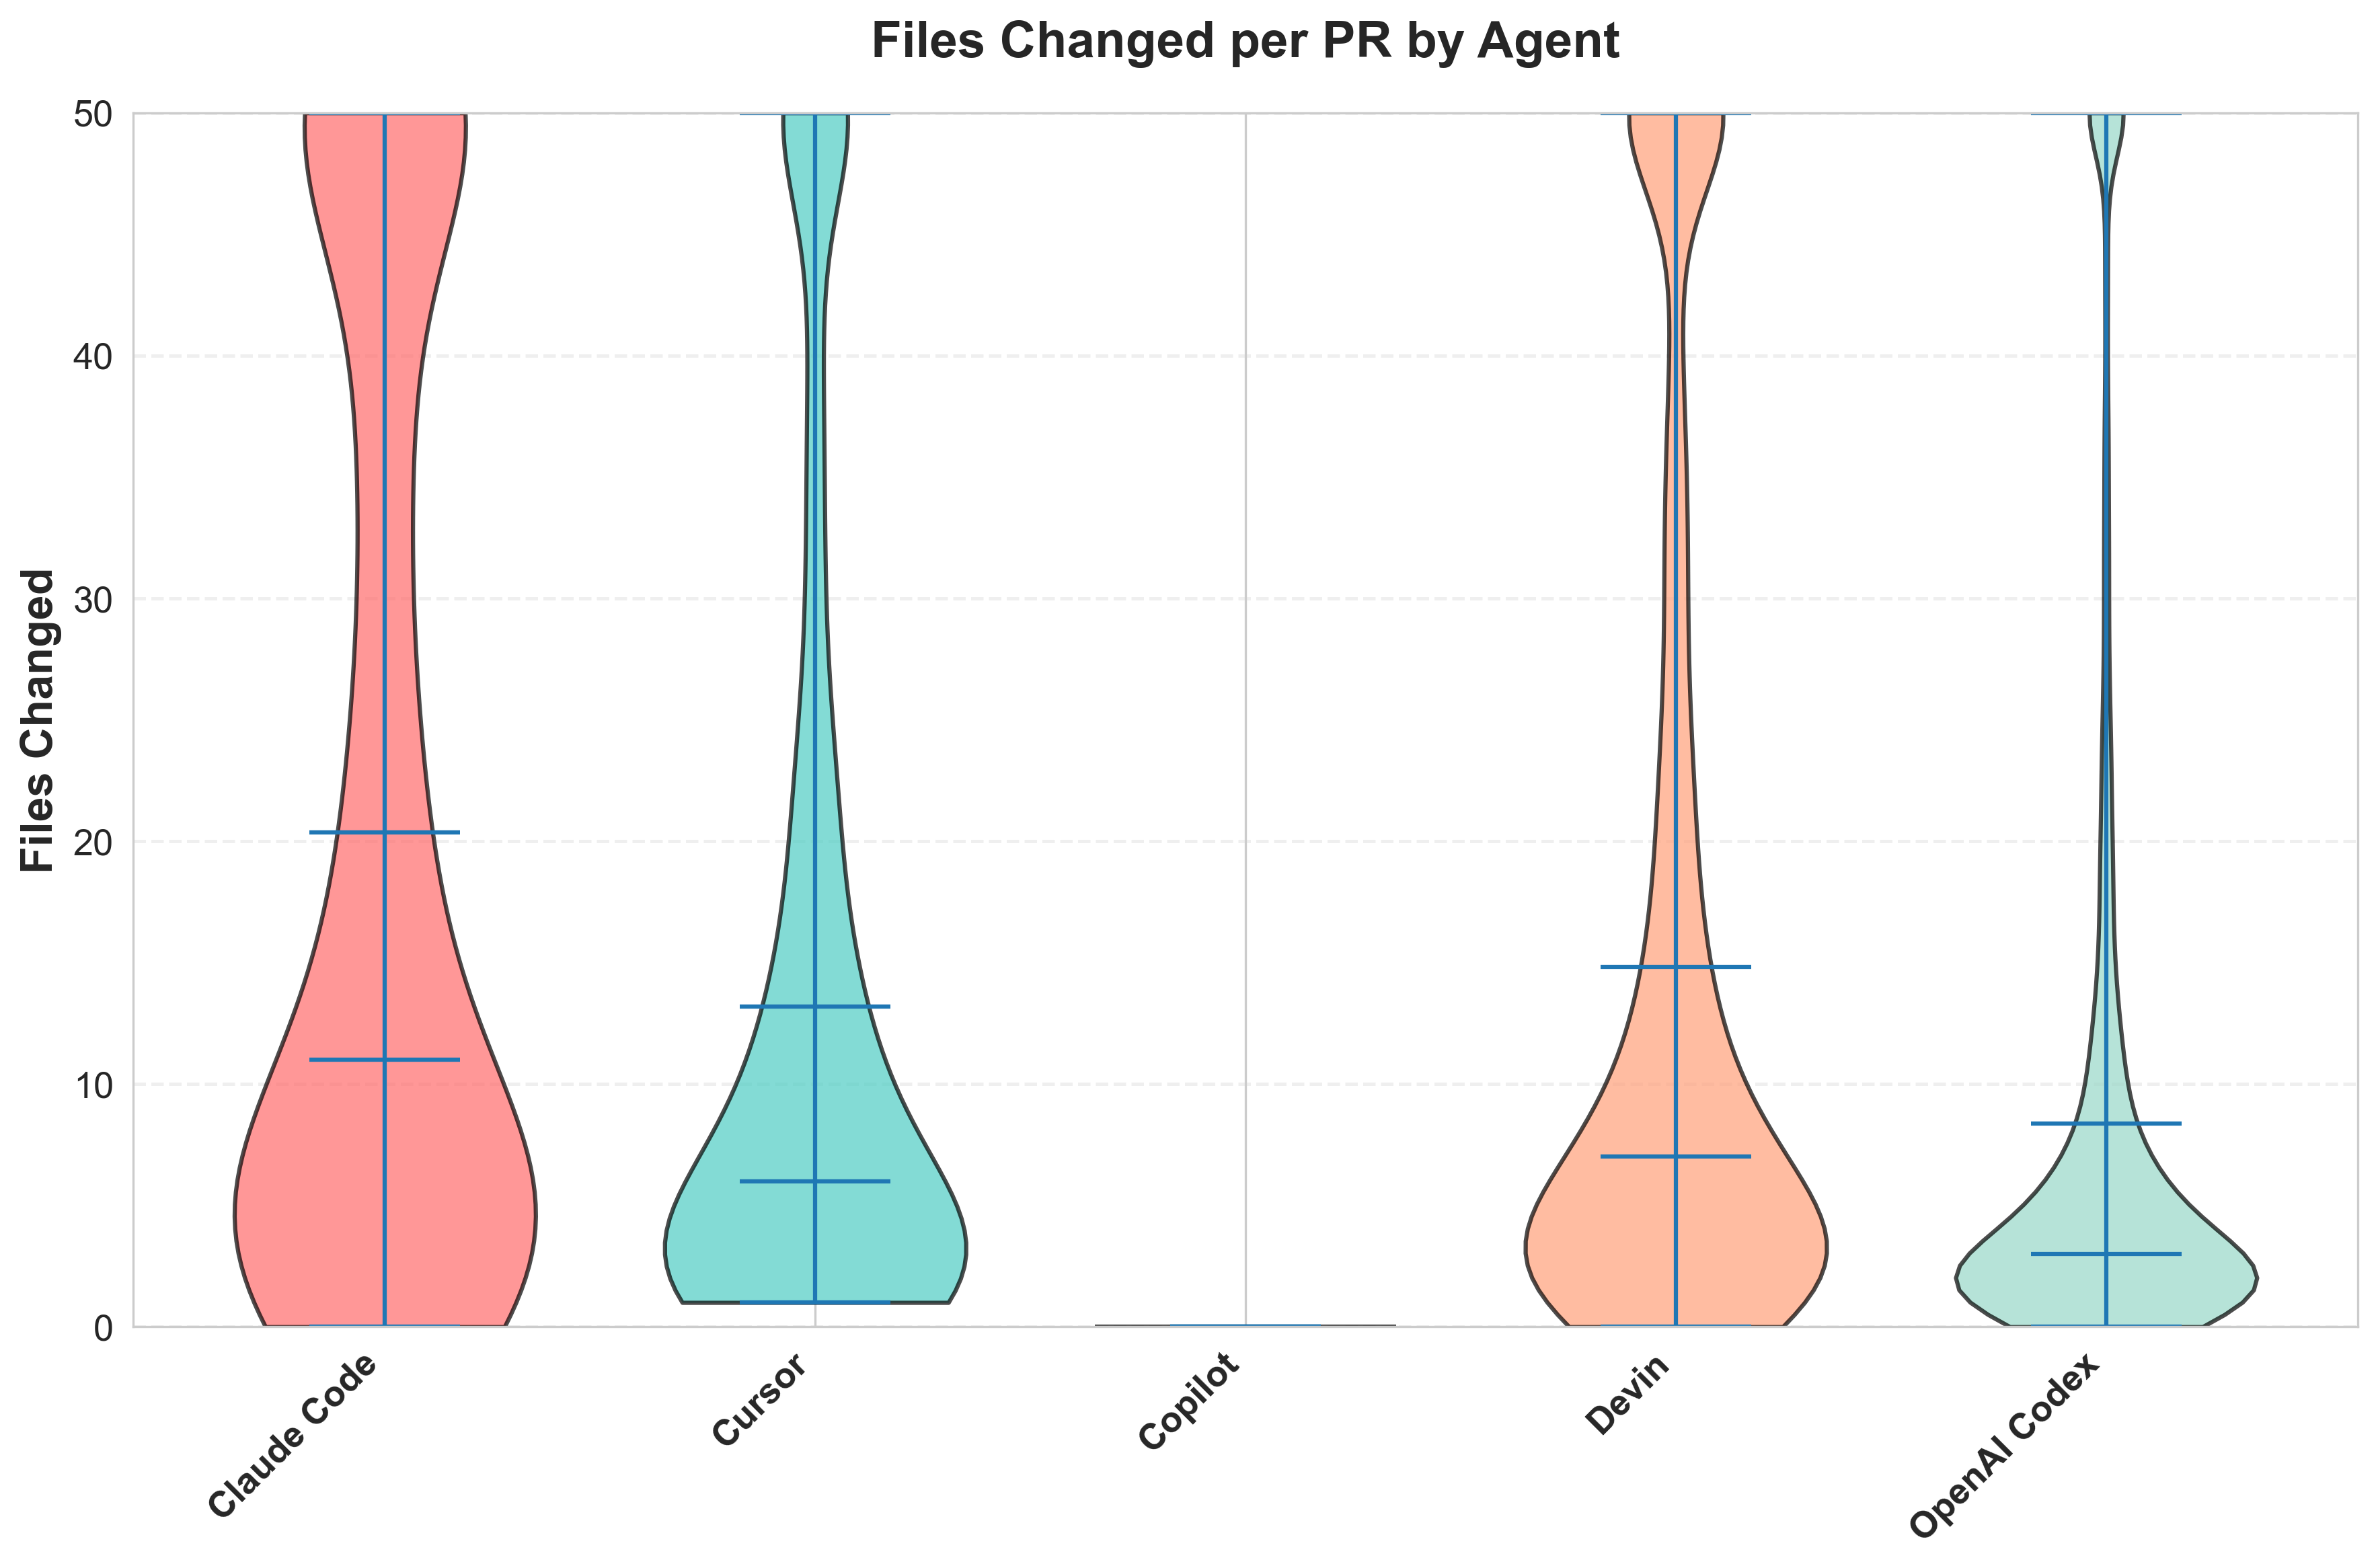
\includegraphics[width=\textwidth]{figures_individual/31_entity_files_changed_by_agent.png}
\caption{Files changed per PR by agent}
\label{fig:entity_files}
\end{subfigure}
\hfill
\begin{subfigure}[b]{0.48\textwidth}
\centering
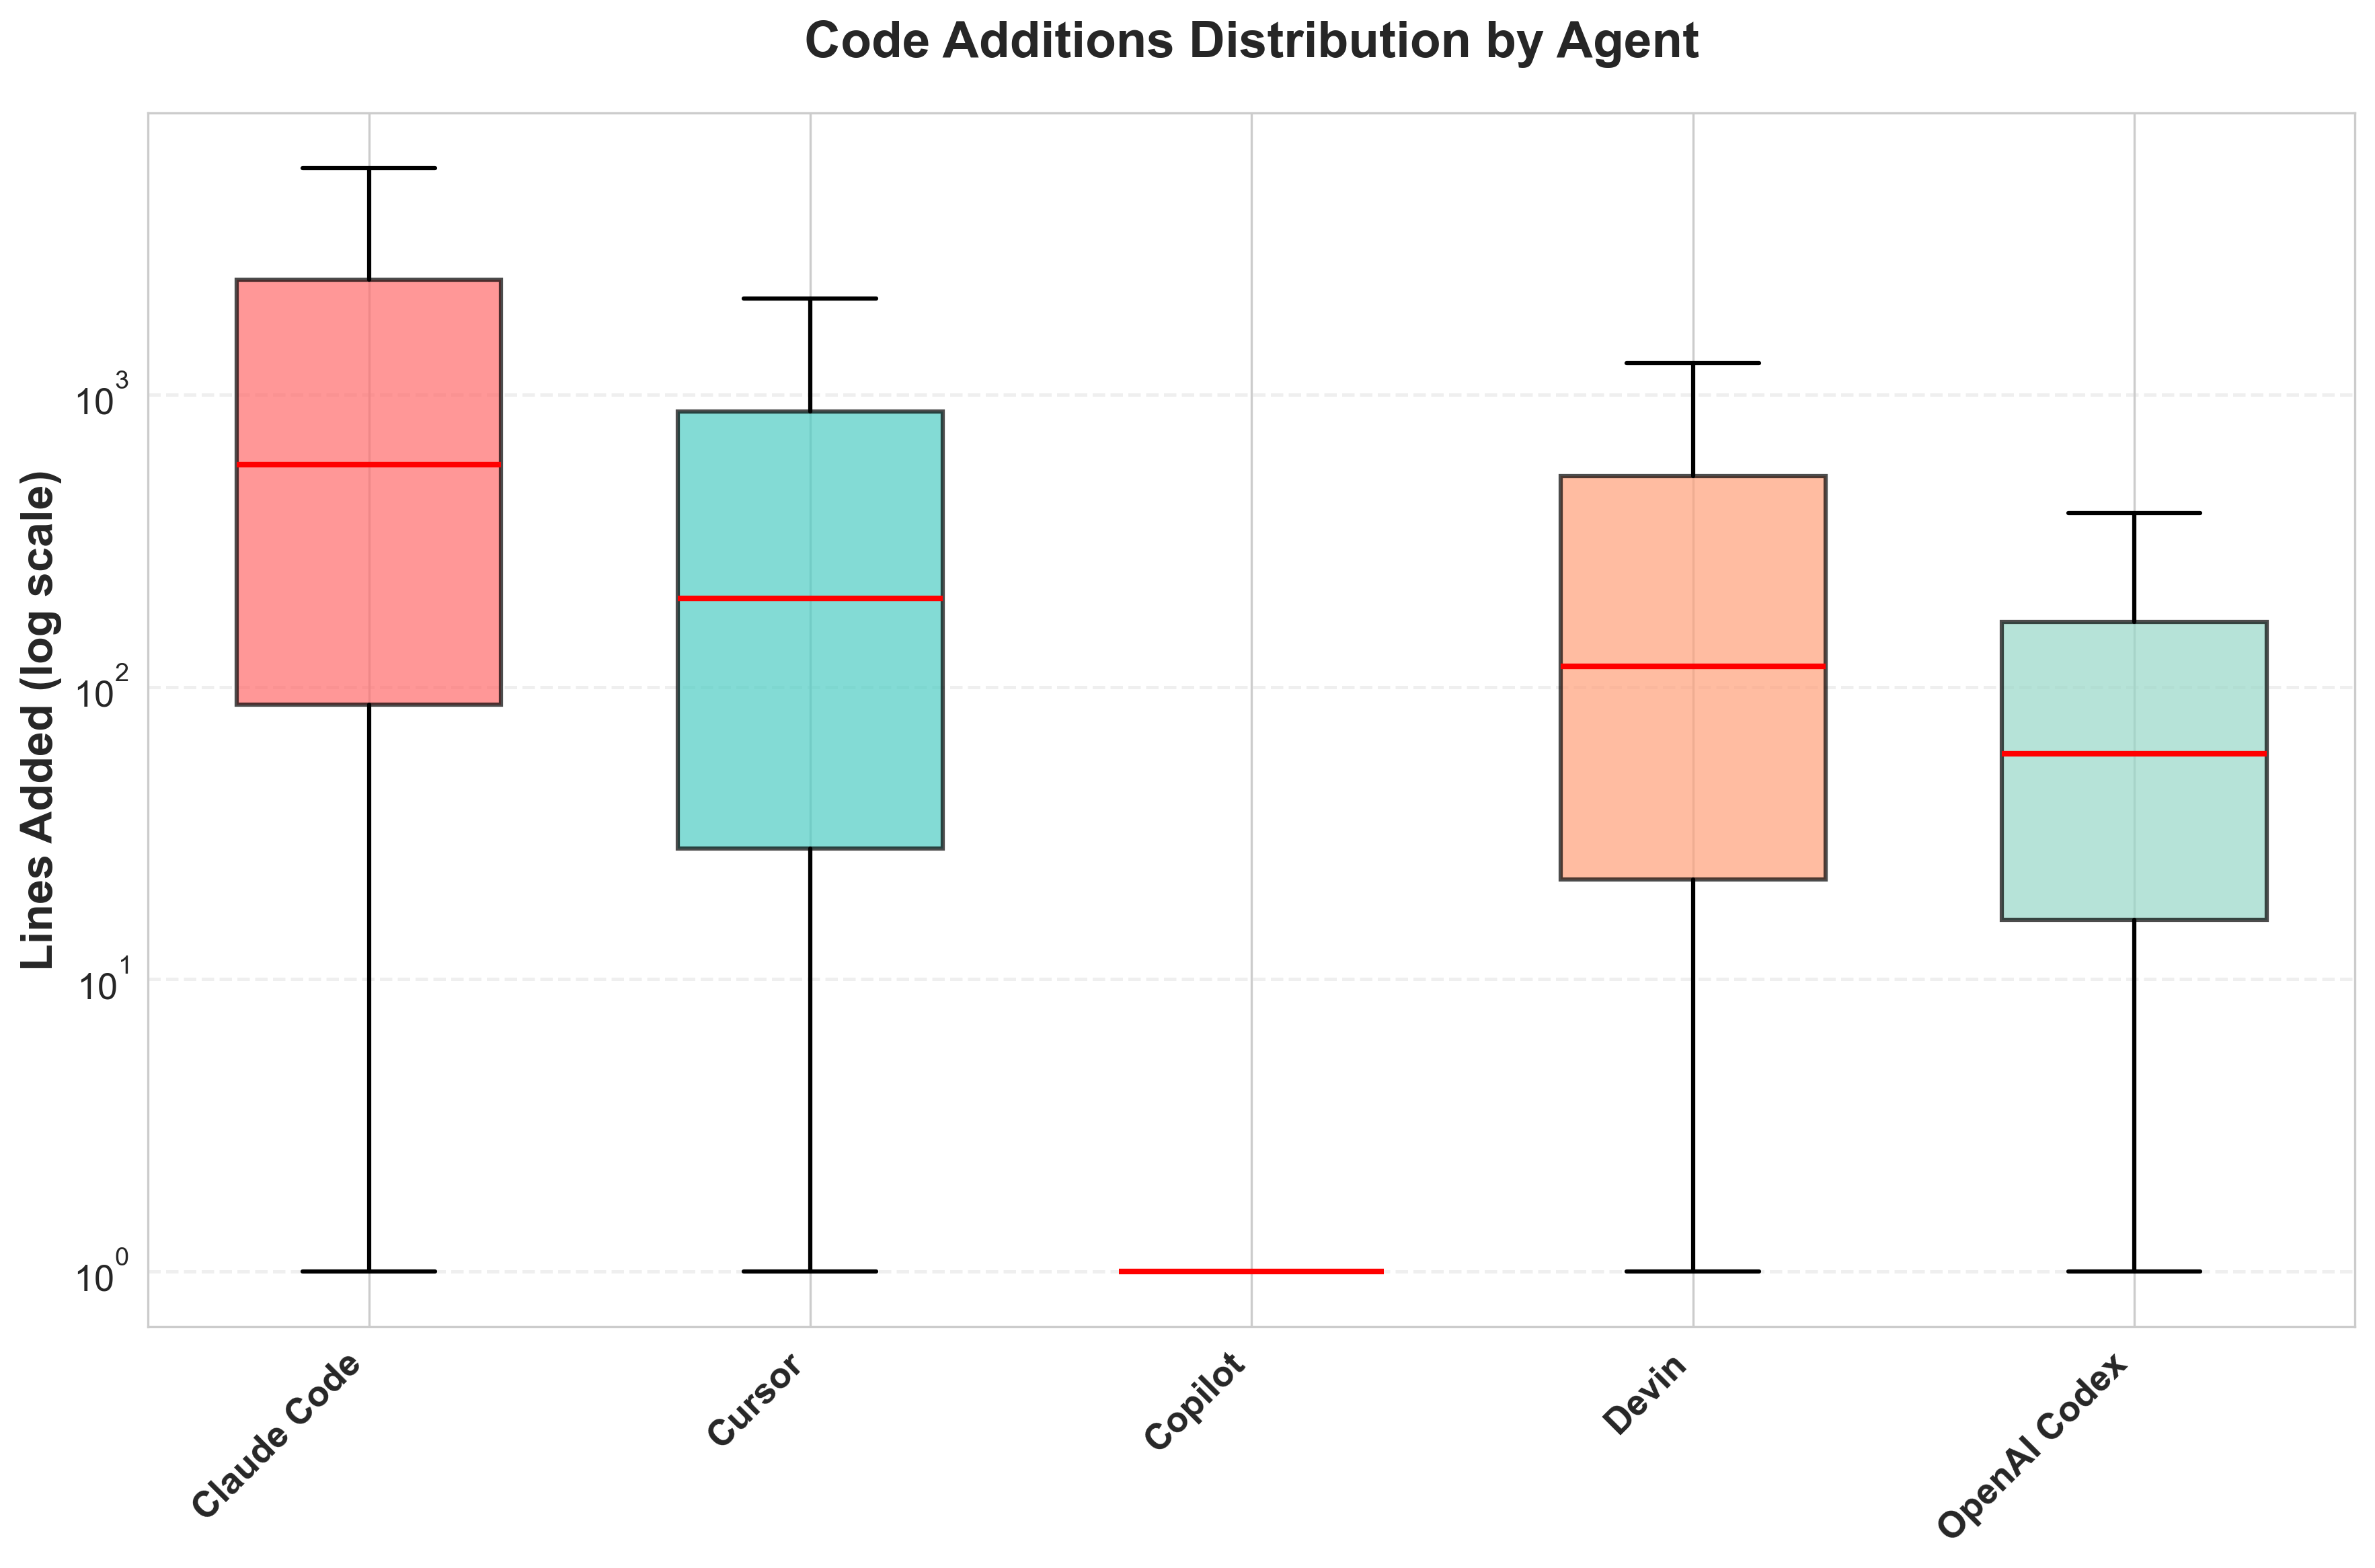
\includegraphics[width=\textwidth]{figures_individual/32_entity_lines_added_by_agent.png}
\caption{Code additions by agent}
\label{fig:entity_additions}
\end{subfigure}

\vspace{0.3cm}

\begin{subfigure}[b]{0.48\textwidth}
\centering
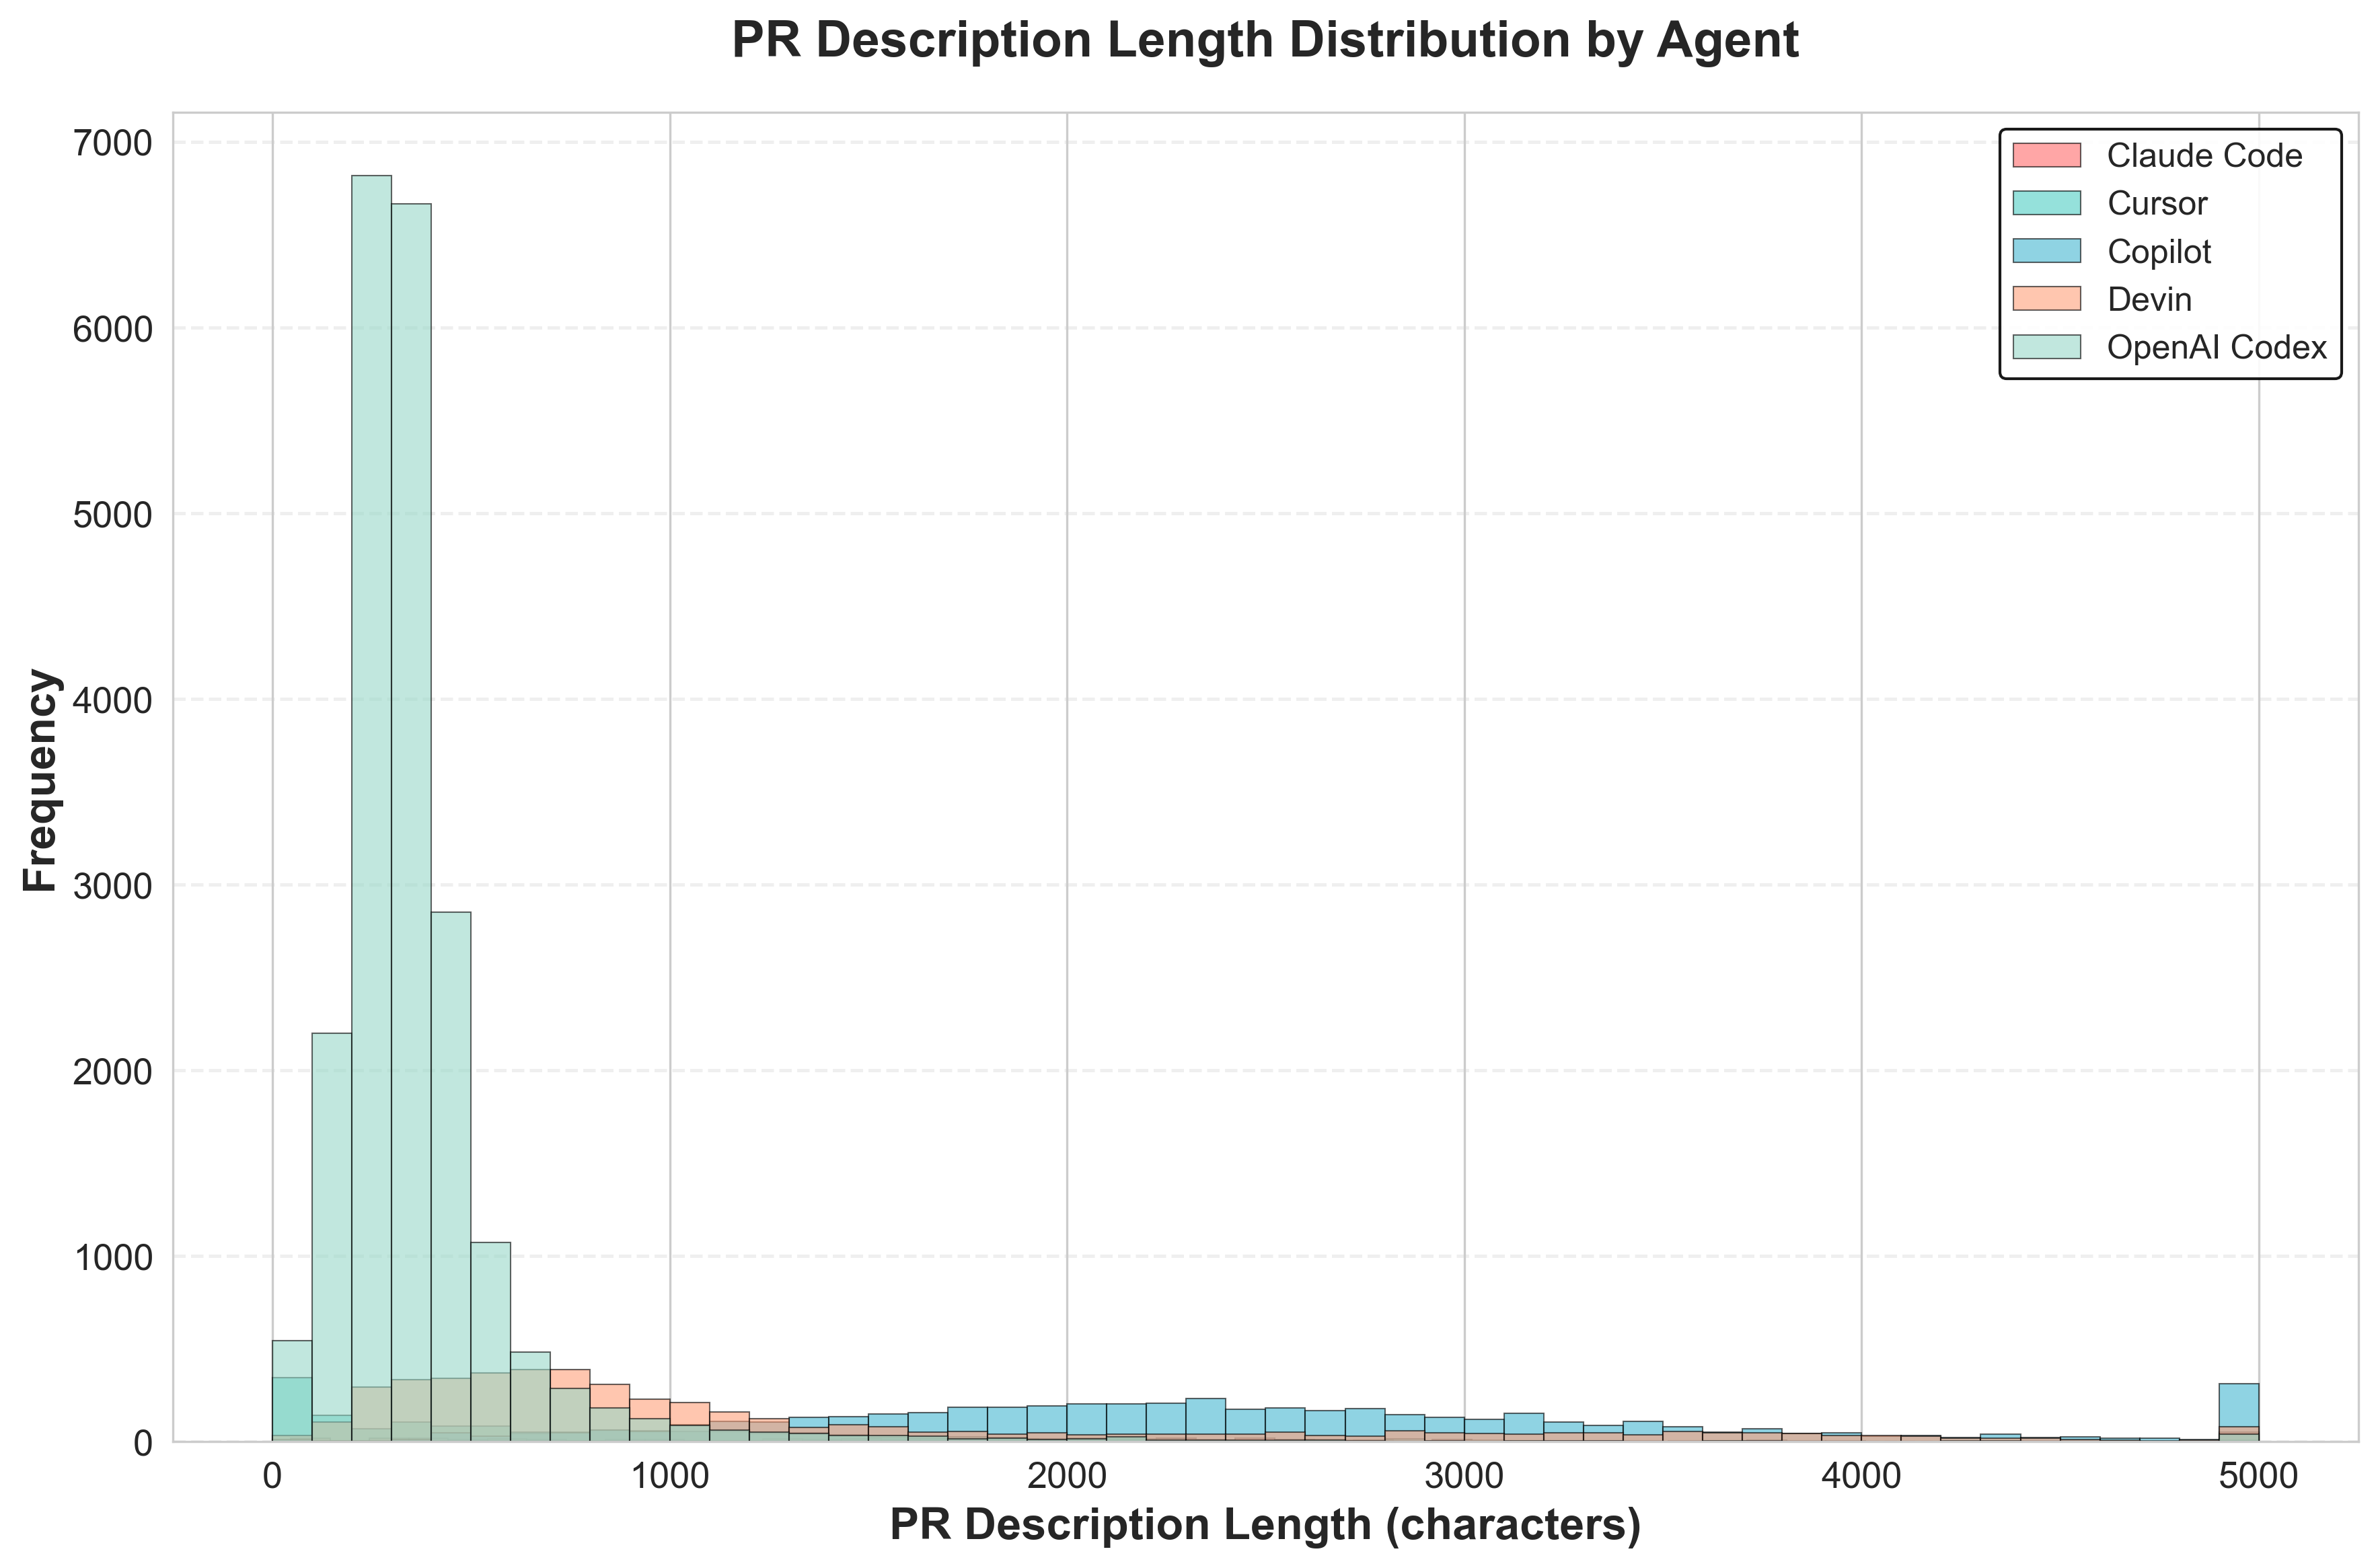
\includegraphics[width=\textwidth]{figures_individual/33_entity_pr_description_length_by_agent.png}
\caption{PR description length by agent}
\label{fig:entity_pr_desc}
\end{subfigure}
\hfill
\begin{subfigure}[b]{0.48\textwidth}
\centering
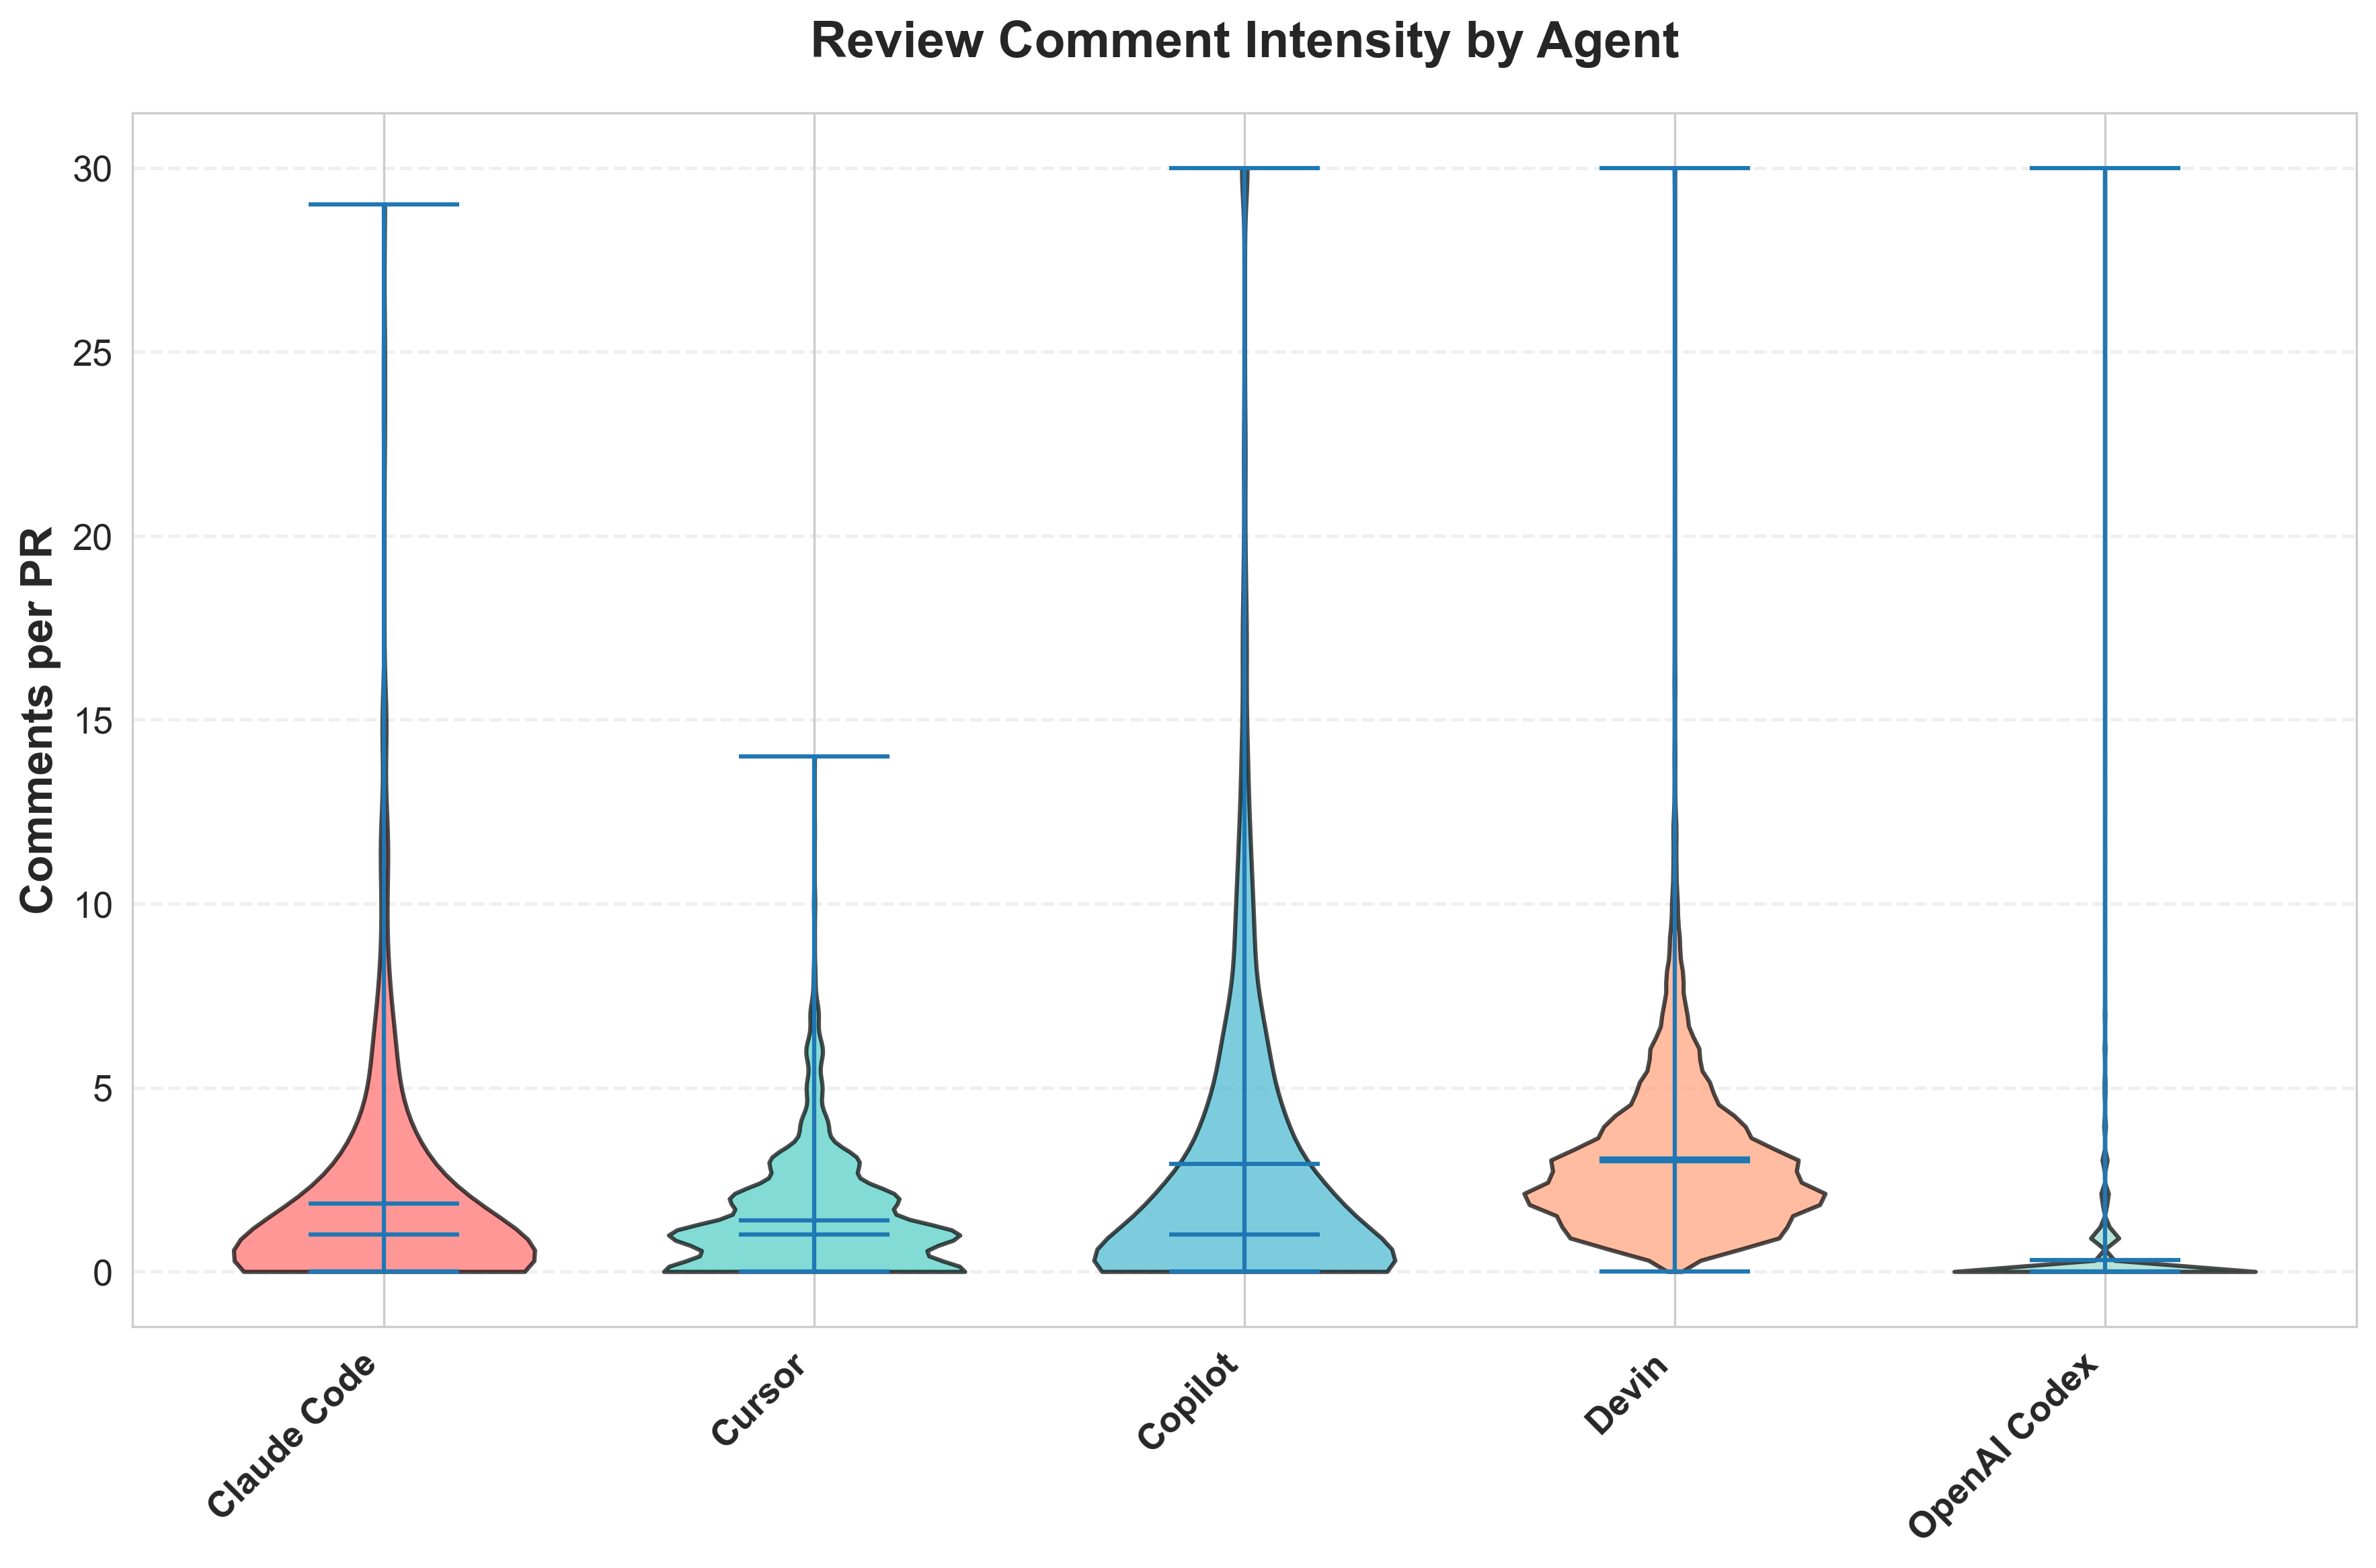
\includegraphics[width=\textwidth]{figures_individual/34_entity_review_comment_intensity_by_agent.png}
\caption{Review comment intensity by agent}
\label{fig:entity_comments}
\end{subfigure}

\vspace{0.3cm}

\begin{subfigure}[b]{0.48\textwidth}
\centering
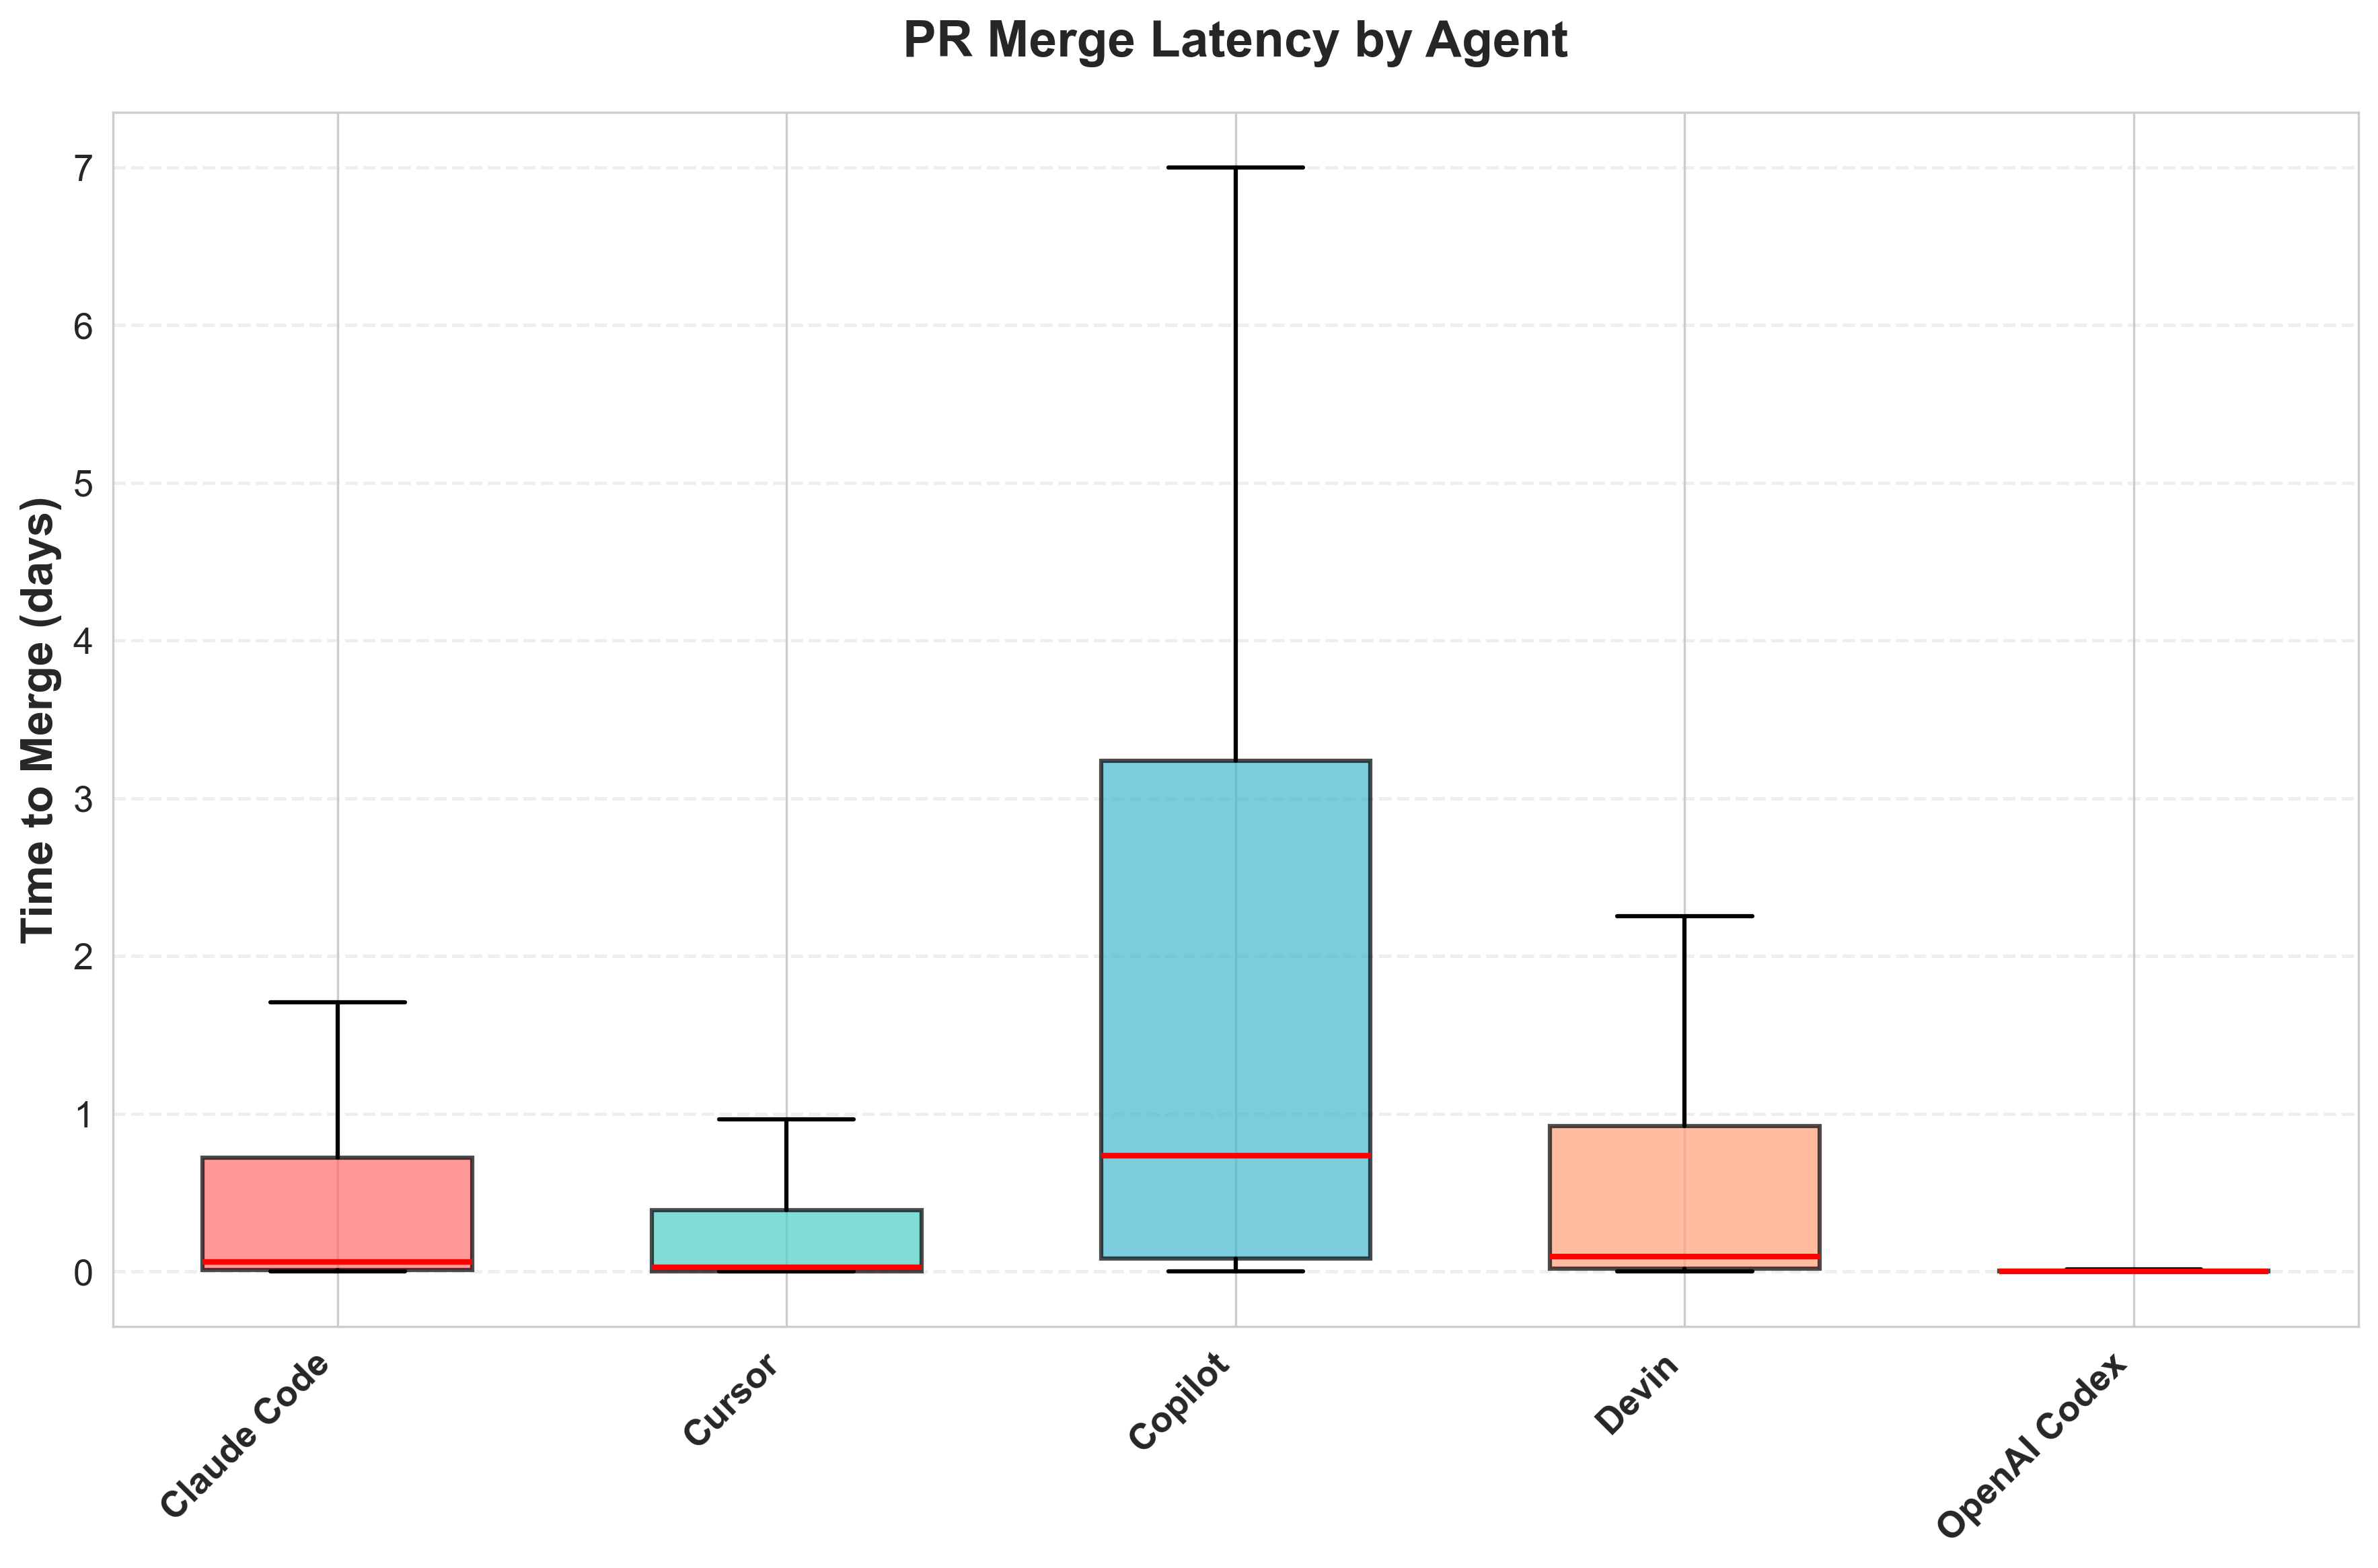
\includegraphics[width=\textwidth]{figures_individual/35_entity_time_to_merge_by_agent.png}
\caption{Time to merge by agent}
\label{fig:entity_merge_time}
\end{subfigure}
\hfill
\begin{subfigure}[b]{0.48\textwidth}
\centering
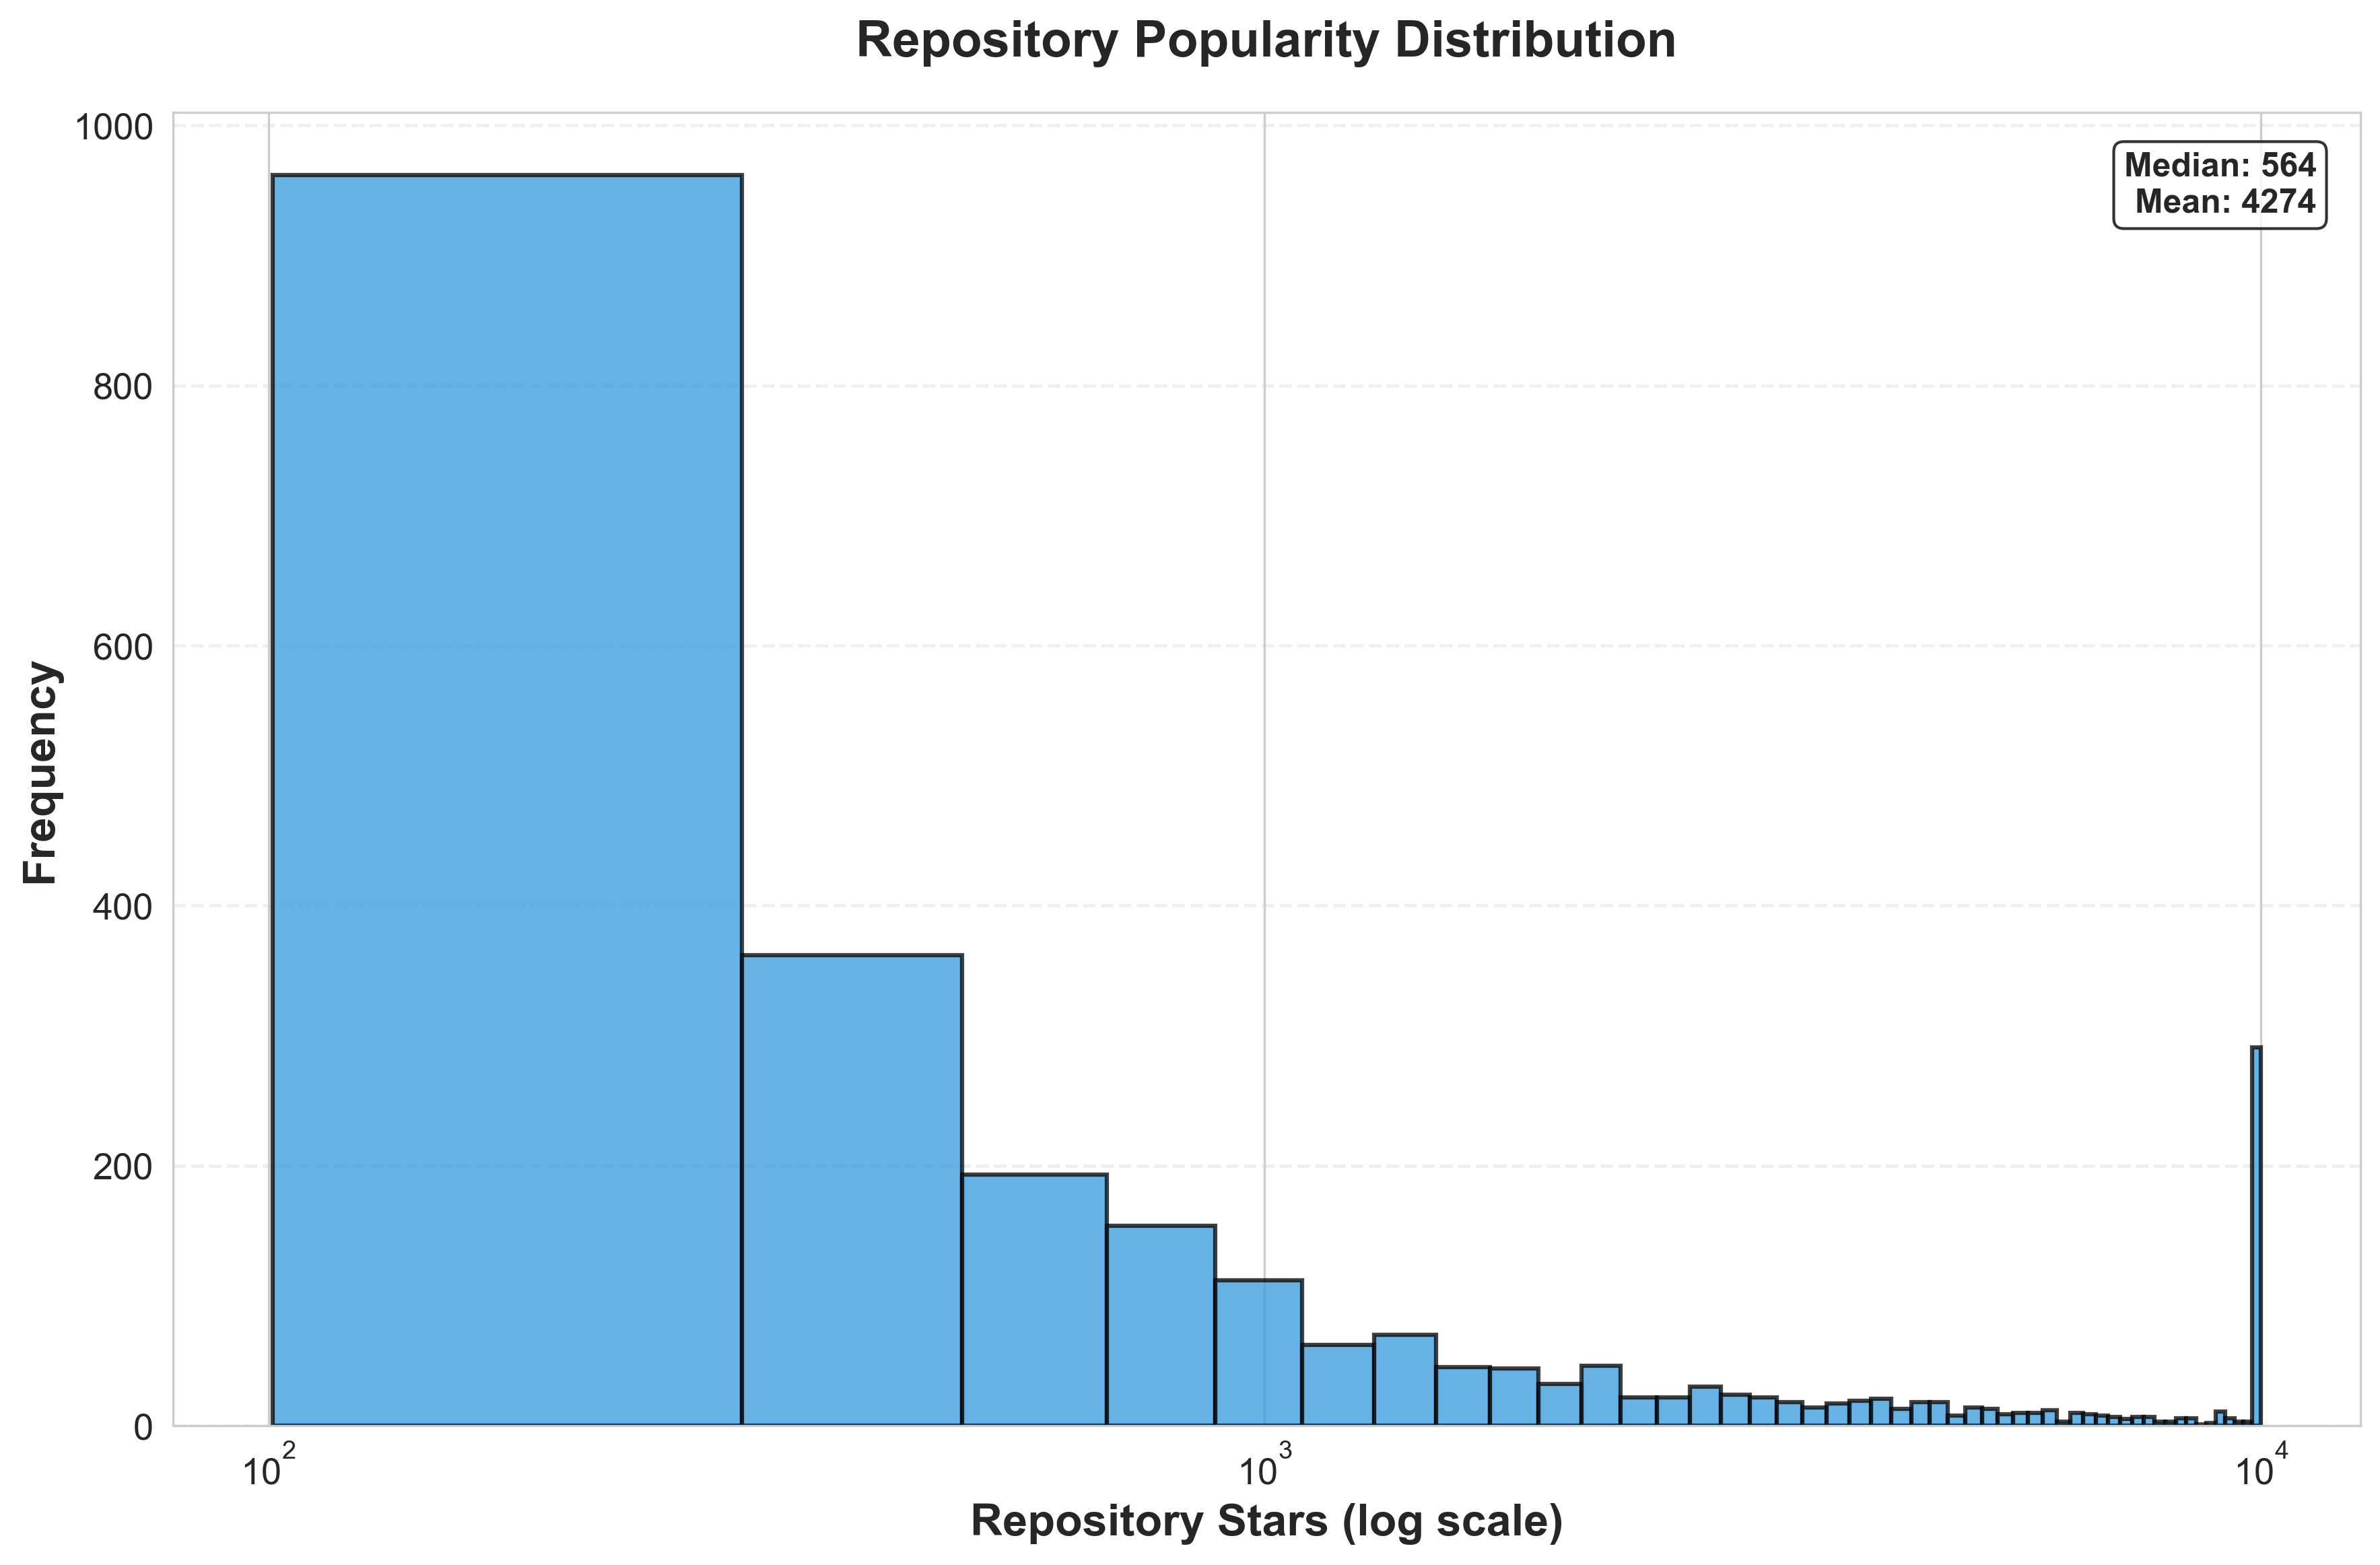
\includegraphics[width=\textwidth]{figures_individual/36_entity_repository_popularity.png}
\caption{Repository popularity distribution}
\label{fig:entity_repo_pop}
\end{subfigure}

\caption{Entity Distributions by Agent (Part 1): Files changed, code additions, PR descriptions, review comments, merge times, and repository popularity. Violin and box plots reveal distinct agent behavior patterns.}
\label{fig:entity_dist_part1}
\end{figure}

\begin{figure}[H]
\centering
\begin{subfigure}[b]{0.48\textwidth}
\centering
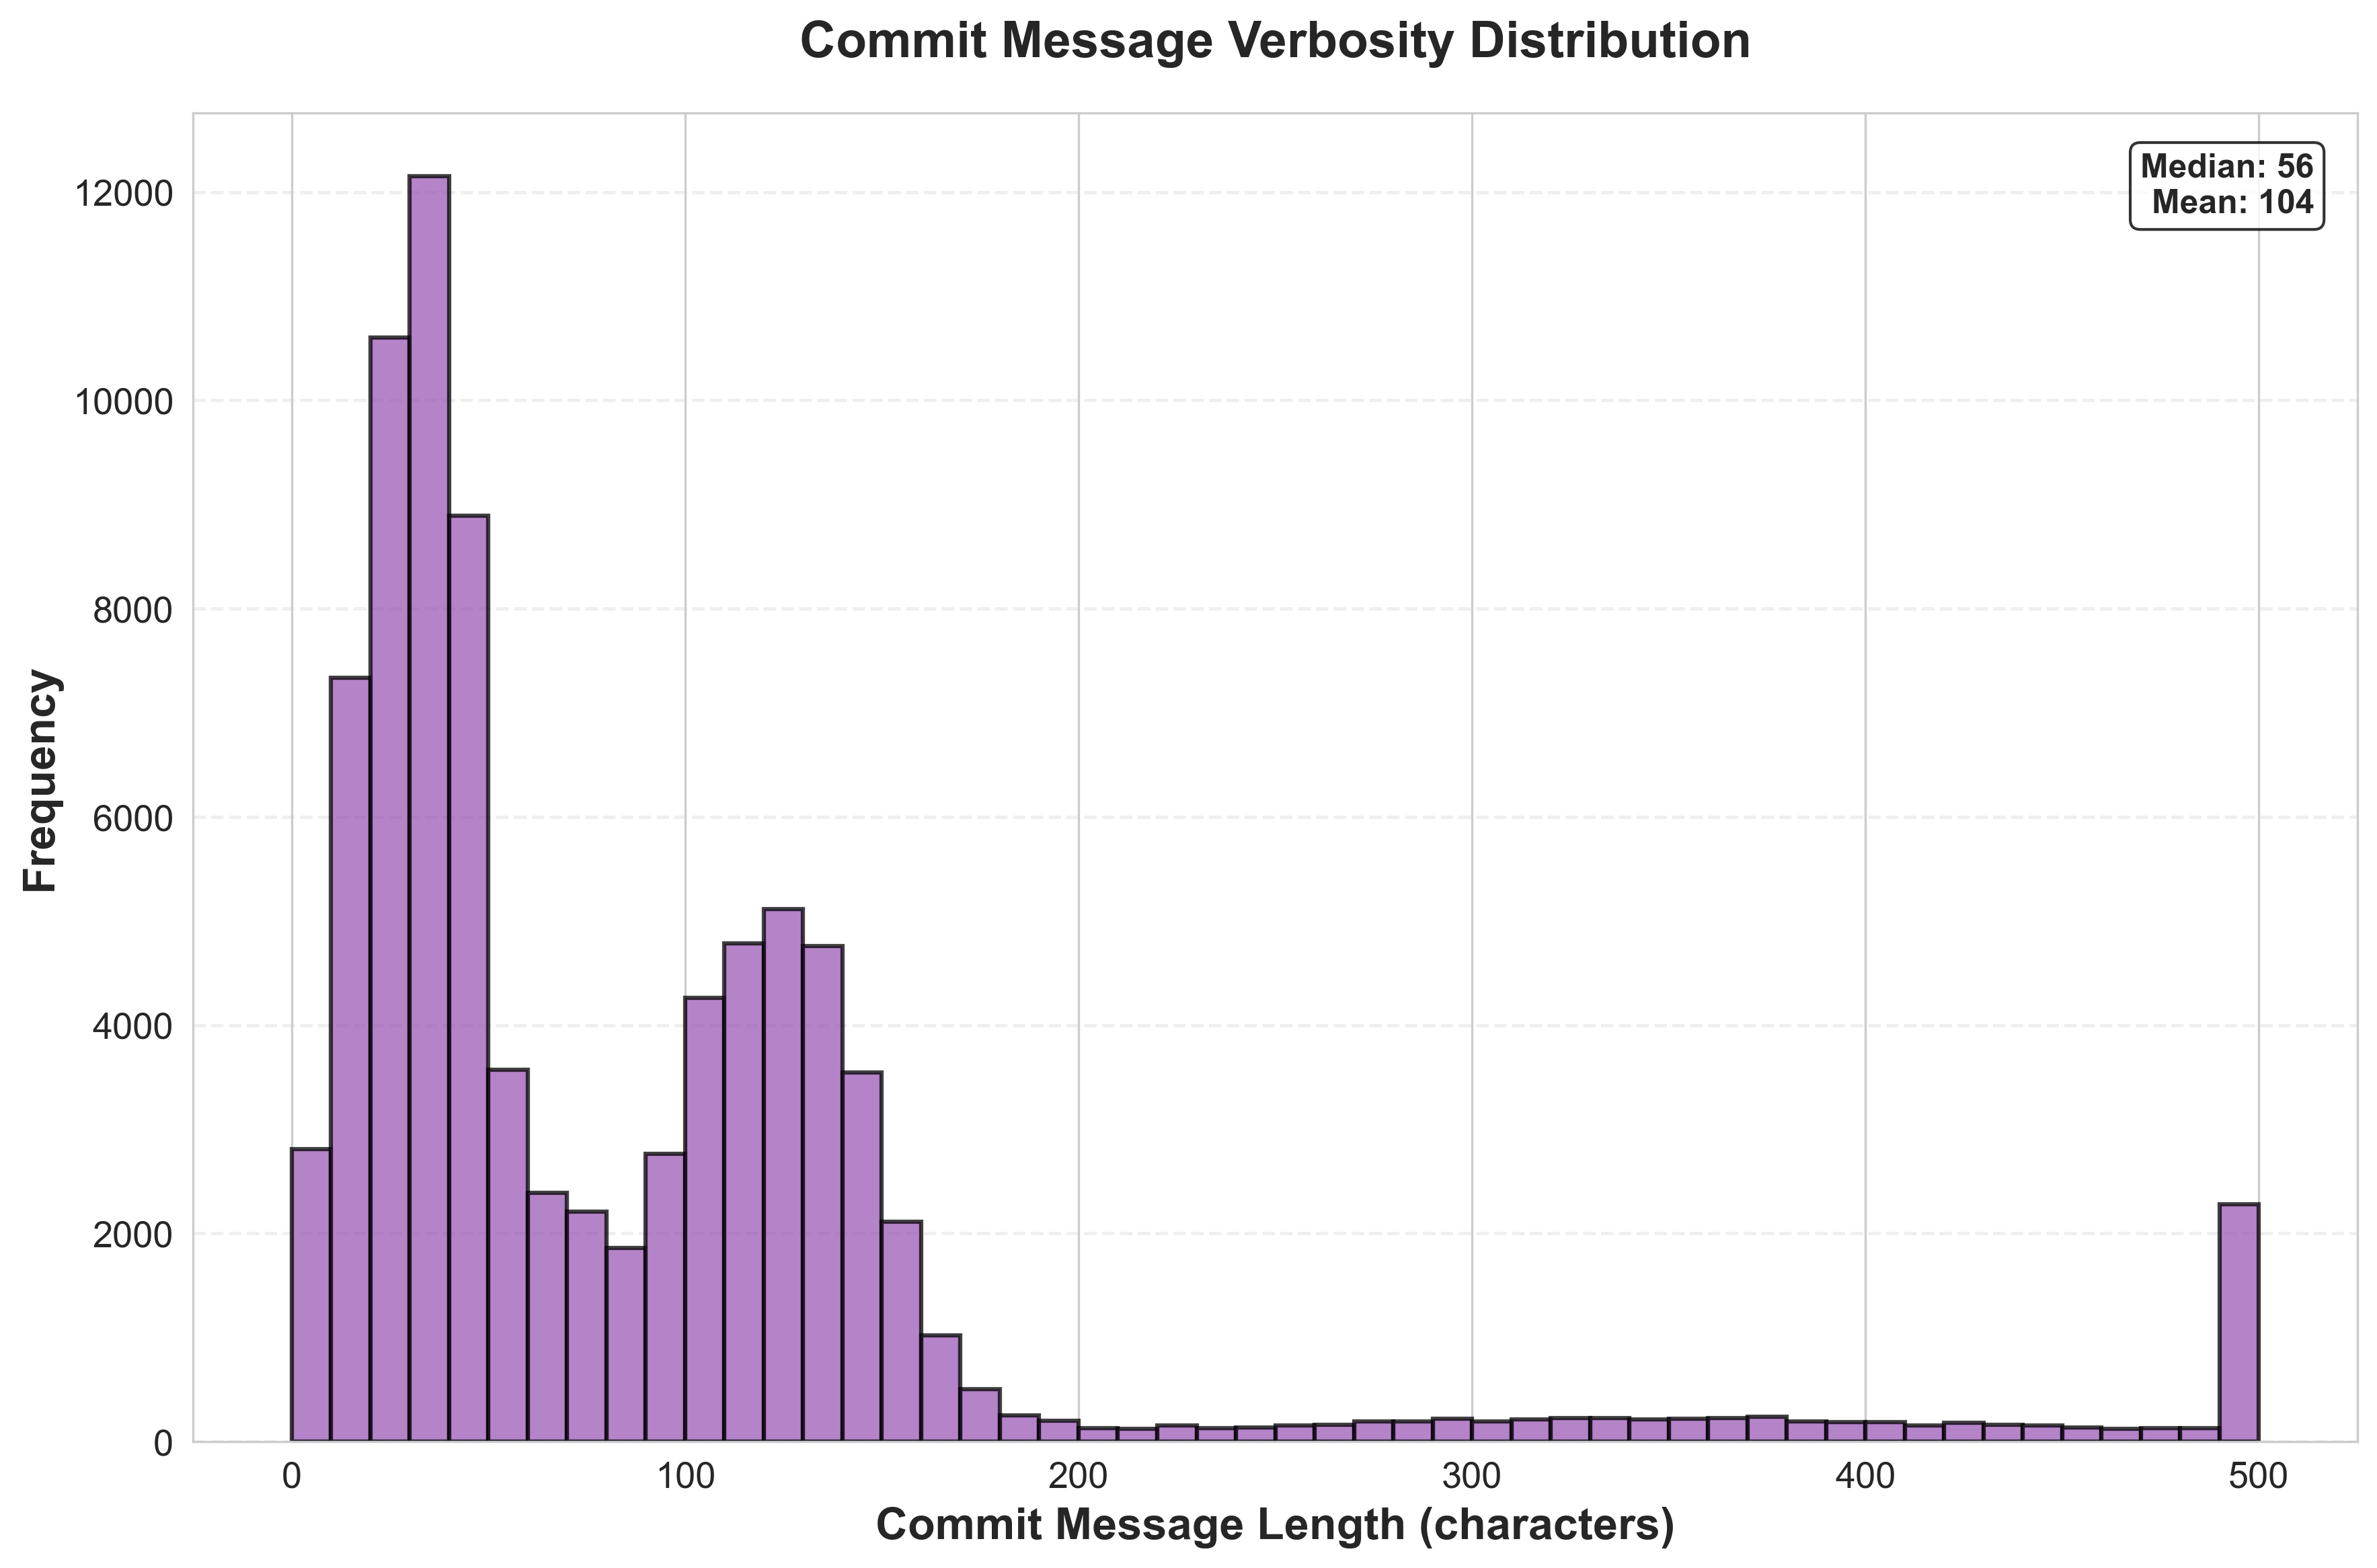
\includegraphics[width=\textwidth]{figures_individual/37_entity_commit_message_verbosity.png}
\caption{Commit message verbosity}
\label{fig:entity_commits}
\end{subfigure}
\hfill
\begin{subfigure}[b]{0.48\textwidth}
\centering
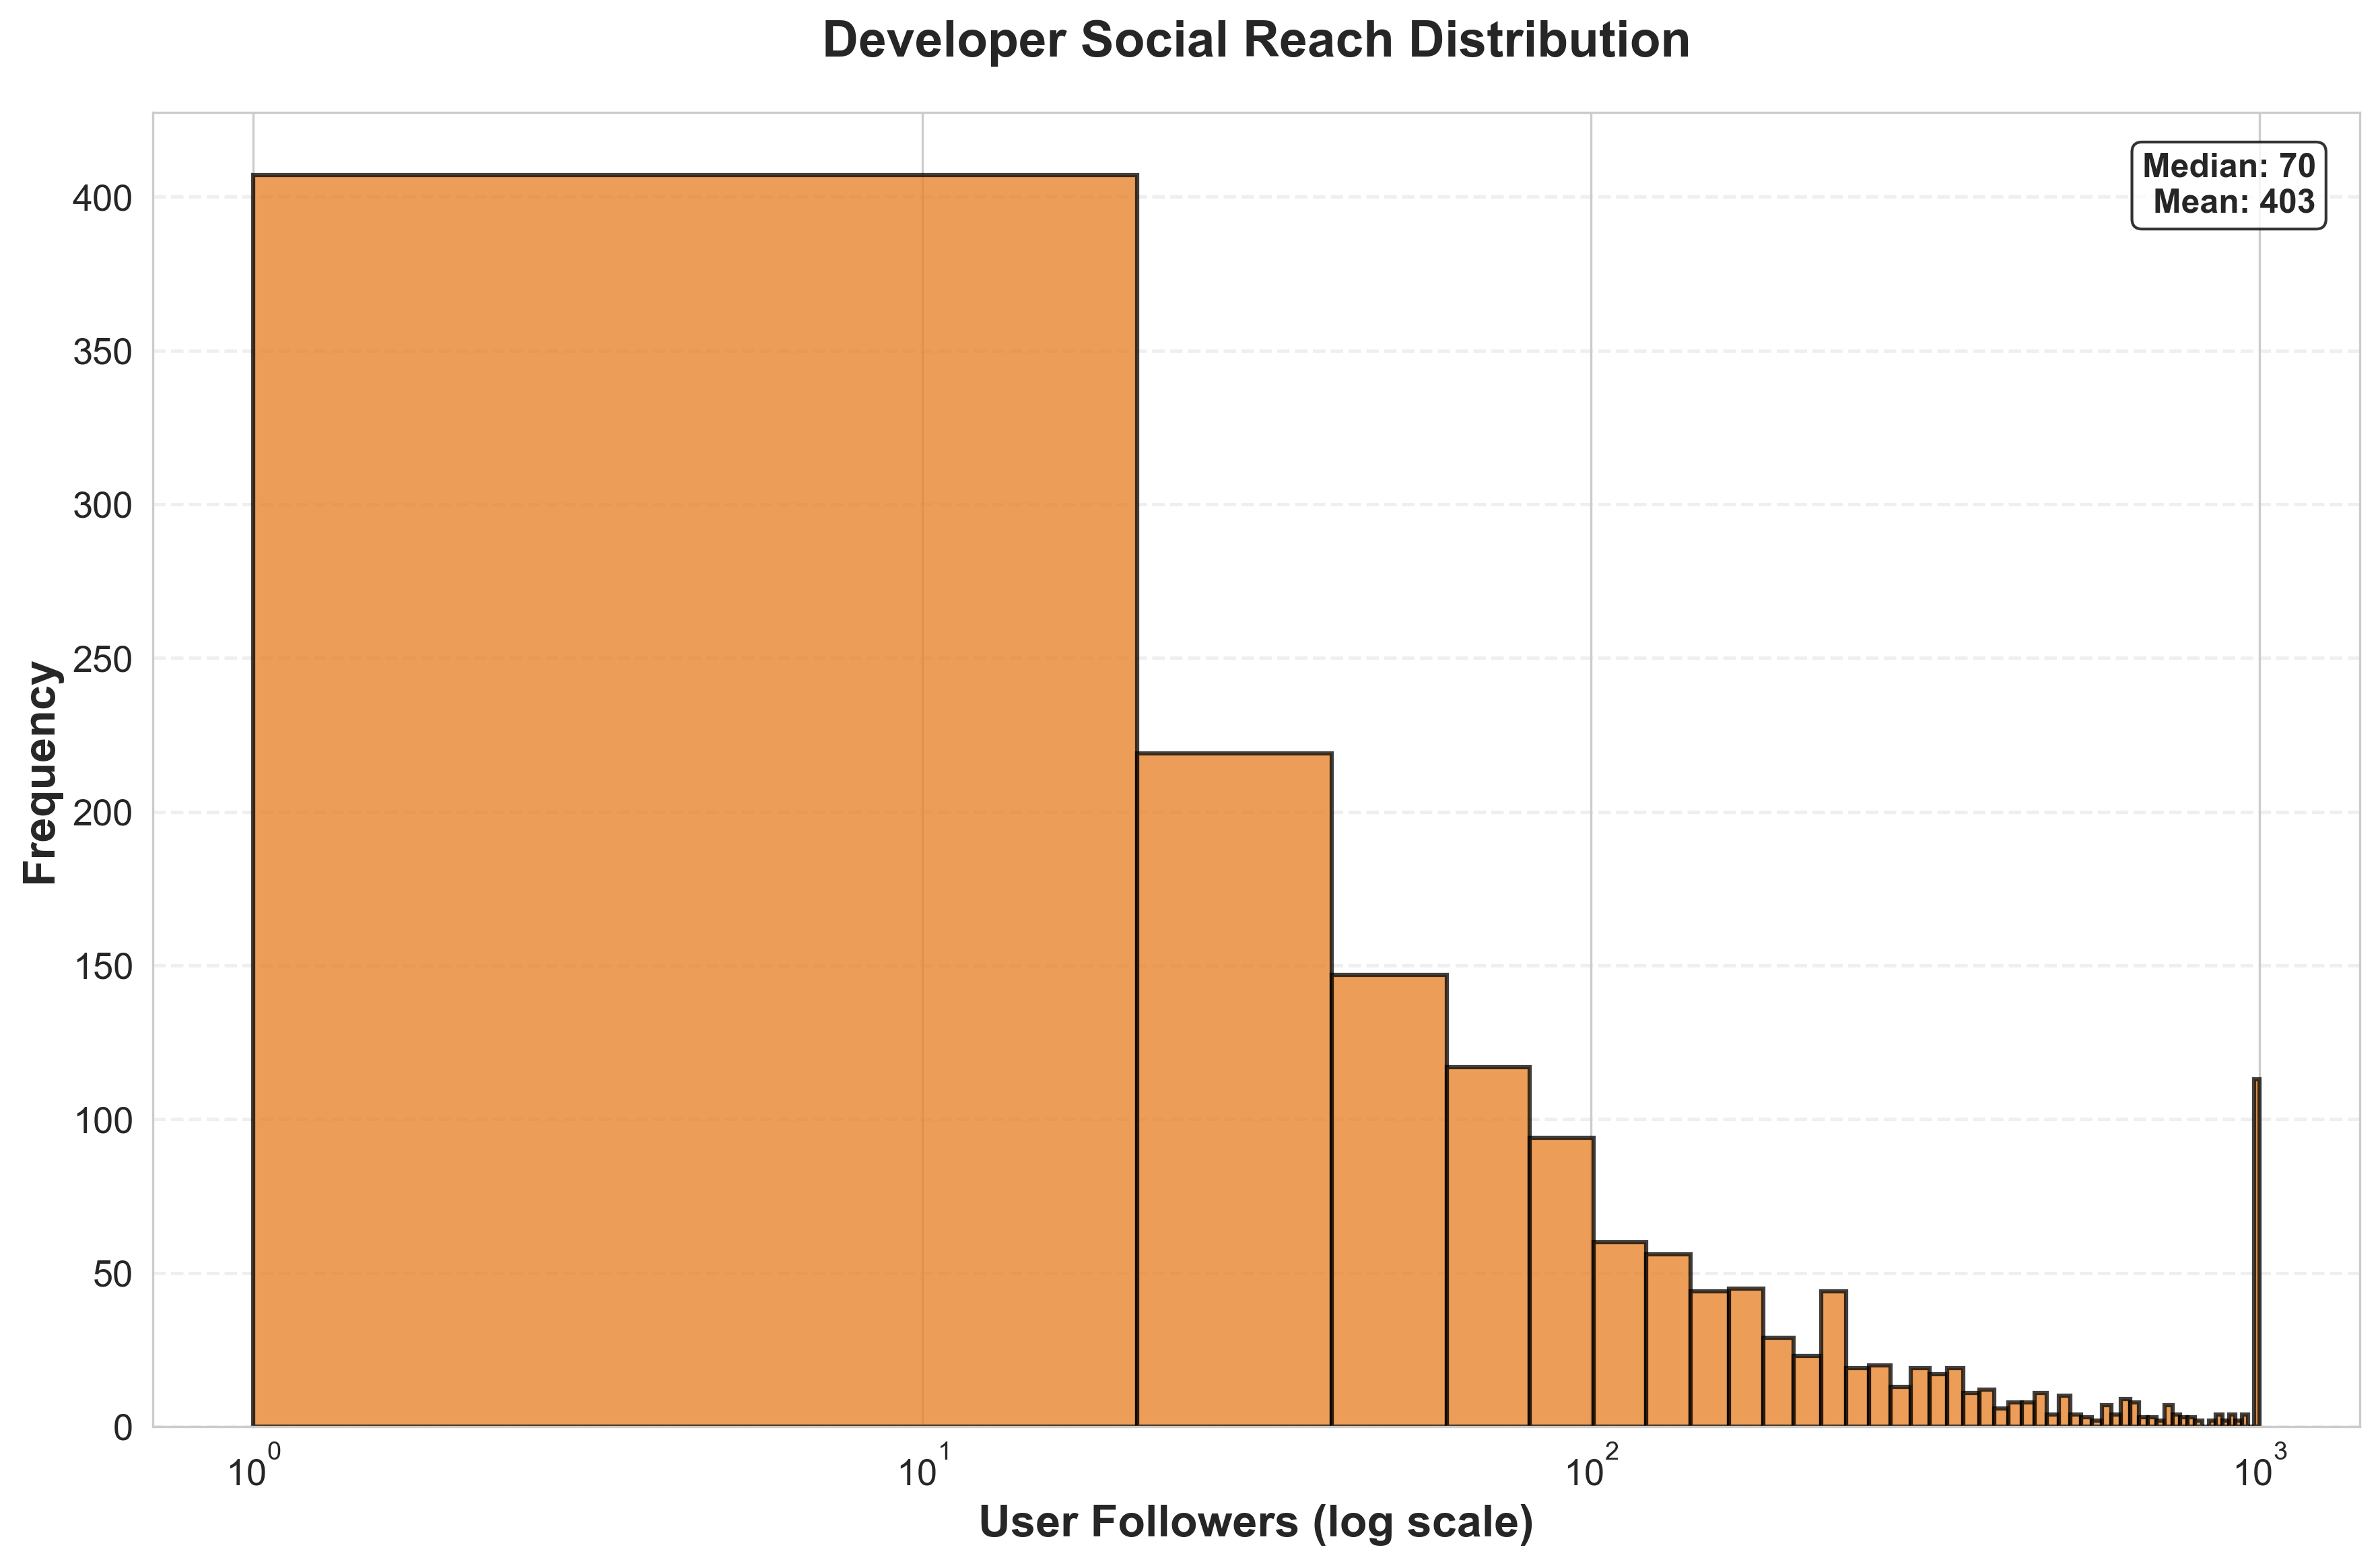
\includegraphics[width=\textwidth]{figures_individual/38_entity_developer_social_reach.png}
\caption{Developer social reach}
\label{fig:entity_social}
\end{subfigure}

\vspace{0.3cm}

\begin{subfigure}[b]{0.48\textwidth}
\centering
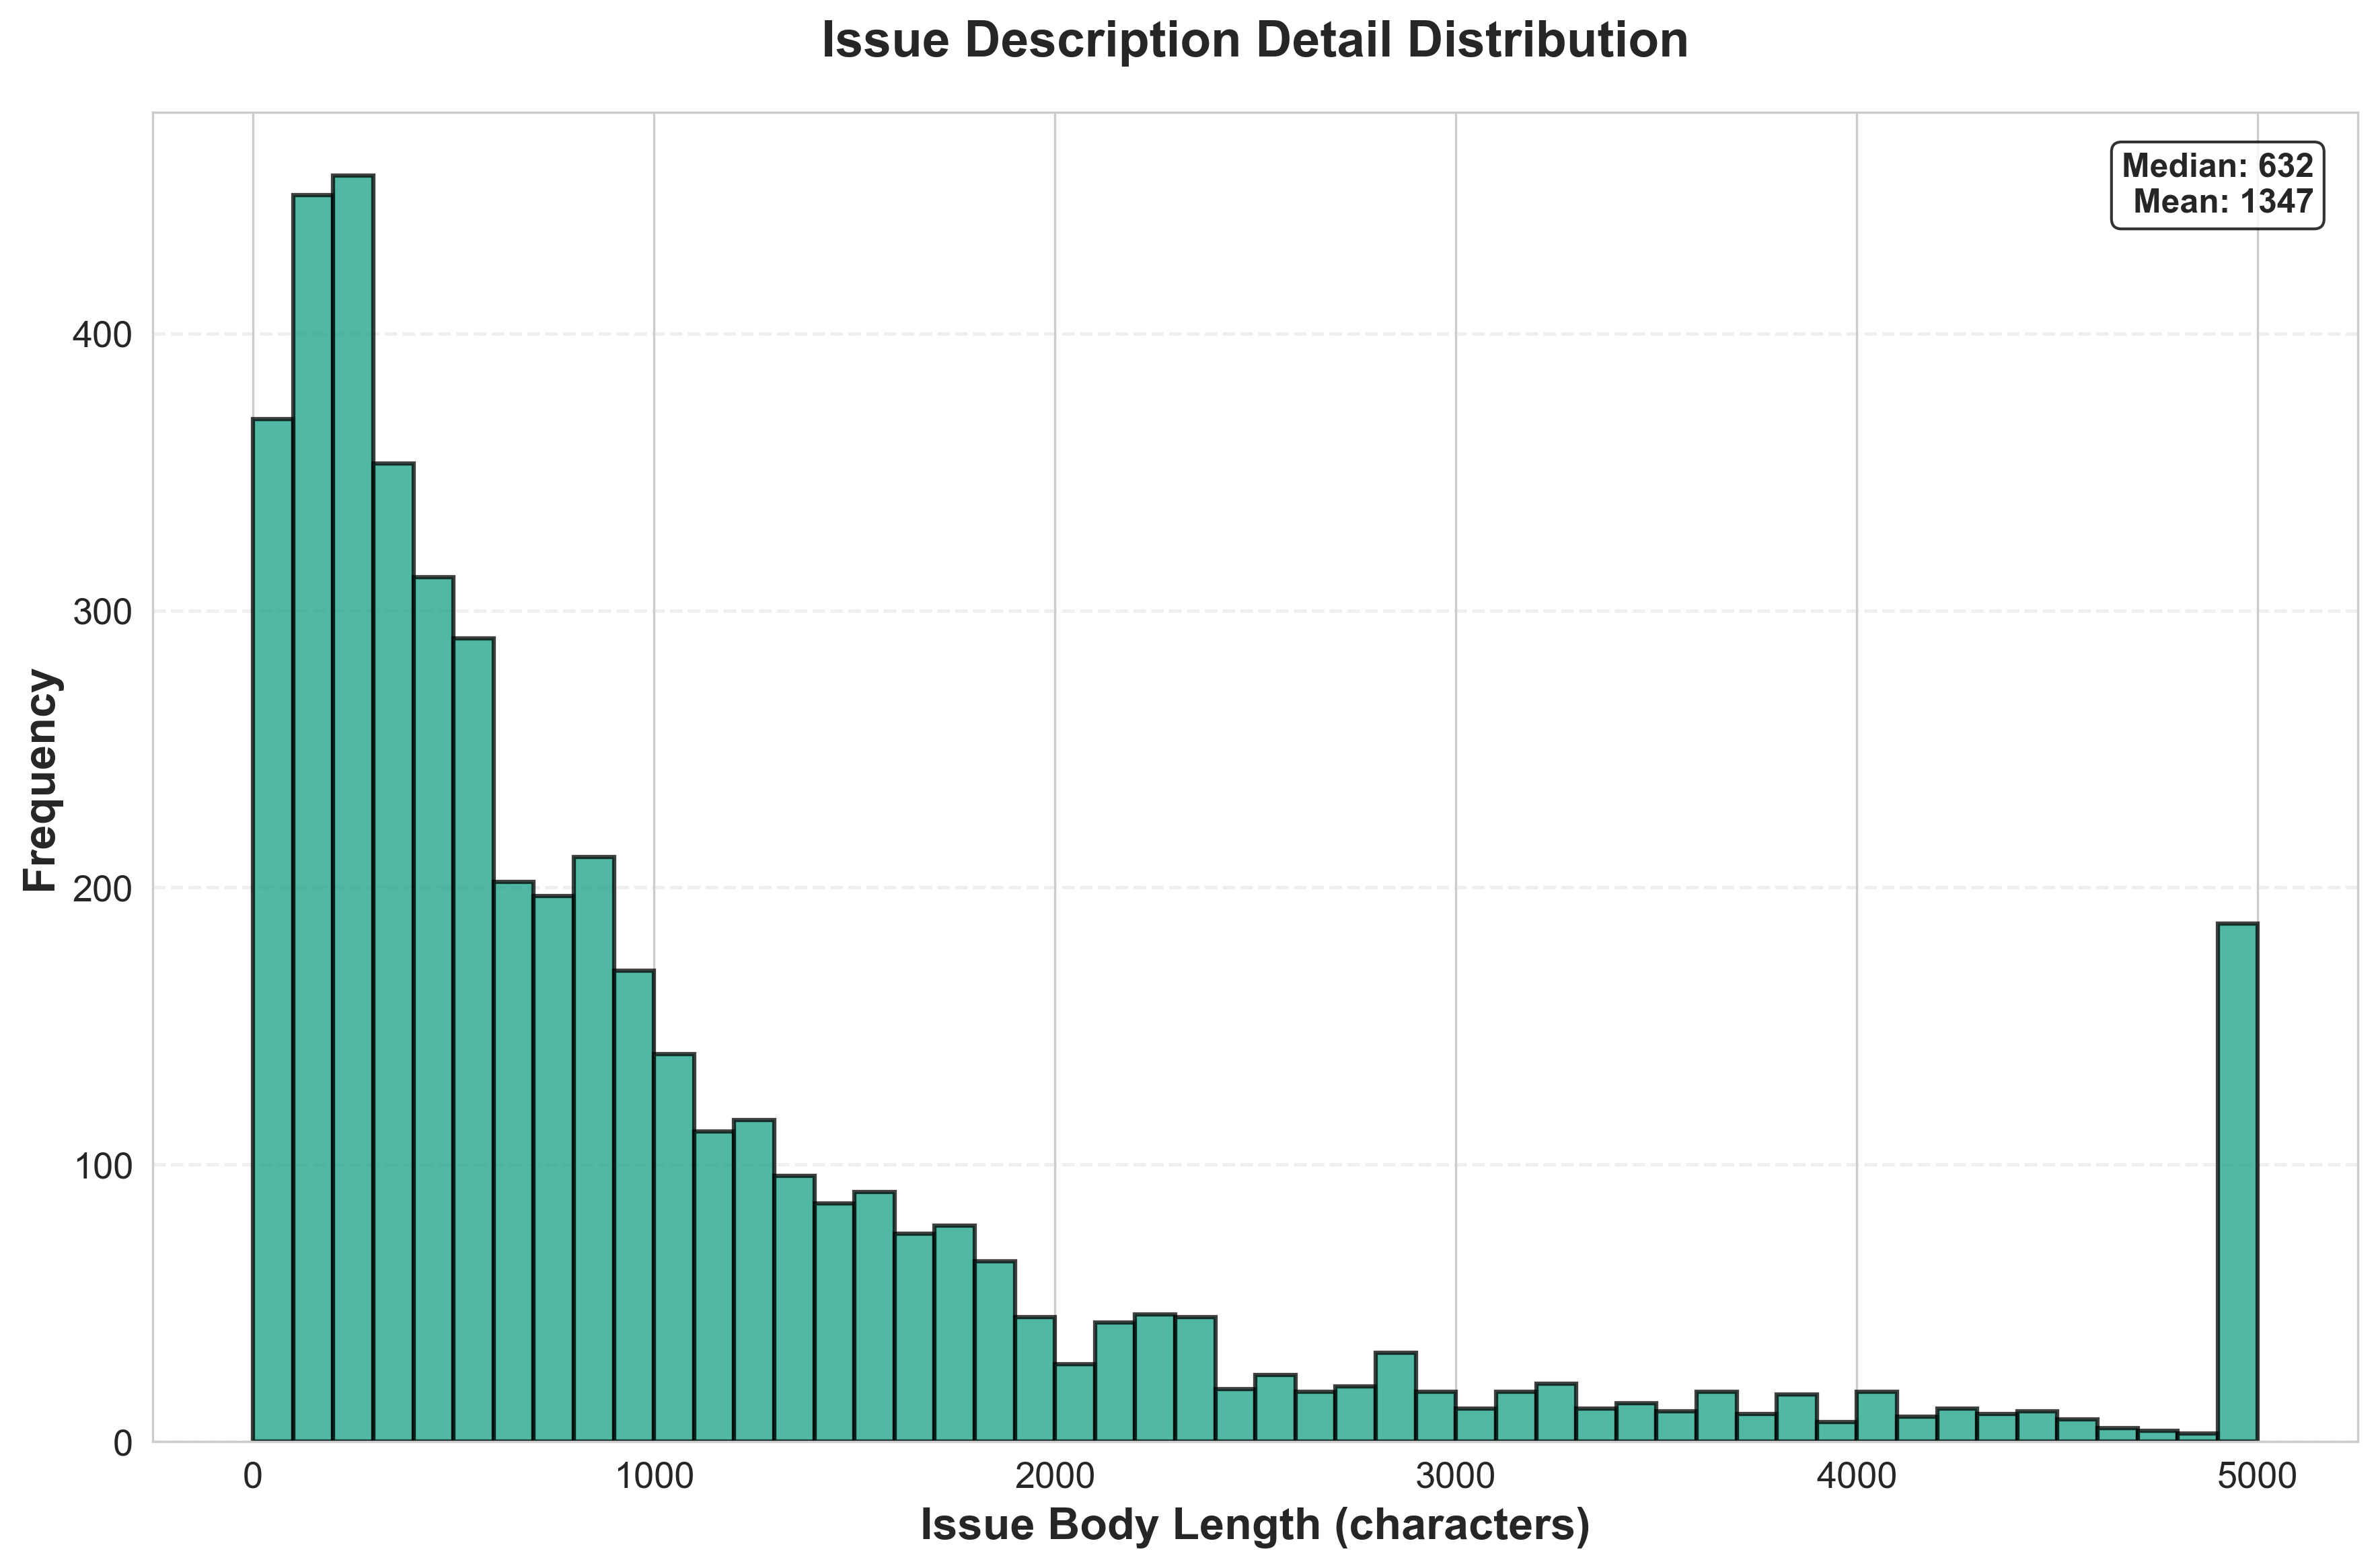
\includegraphics[width=\textwidth]{figures_individual/39_entity_issue_description_detail.png}
\caption{Issue description detail}
\label{fig:entity_issue}
\end{subfigure}

\caption{Entity Distributions by Agent (Part 2): Commit message lengths, developer social reach, issue detail}
\label{fig:entity_dist_part2}
\end{figure}

\begin{figure}[H]
\centering
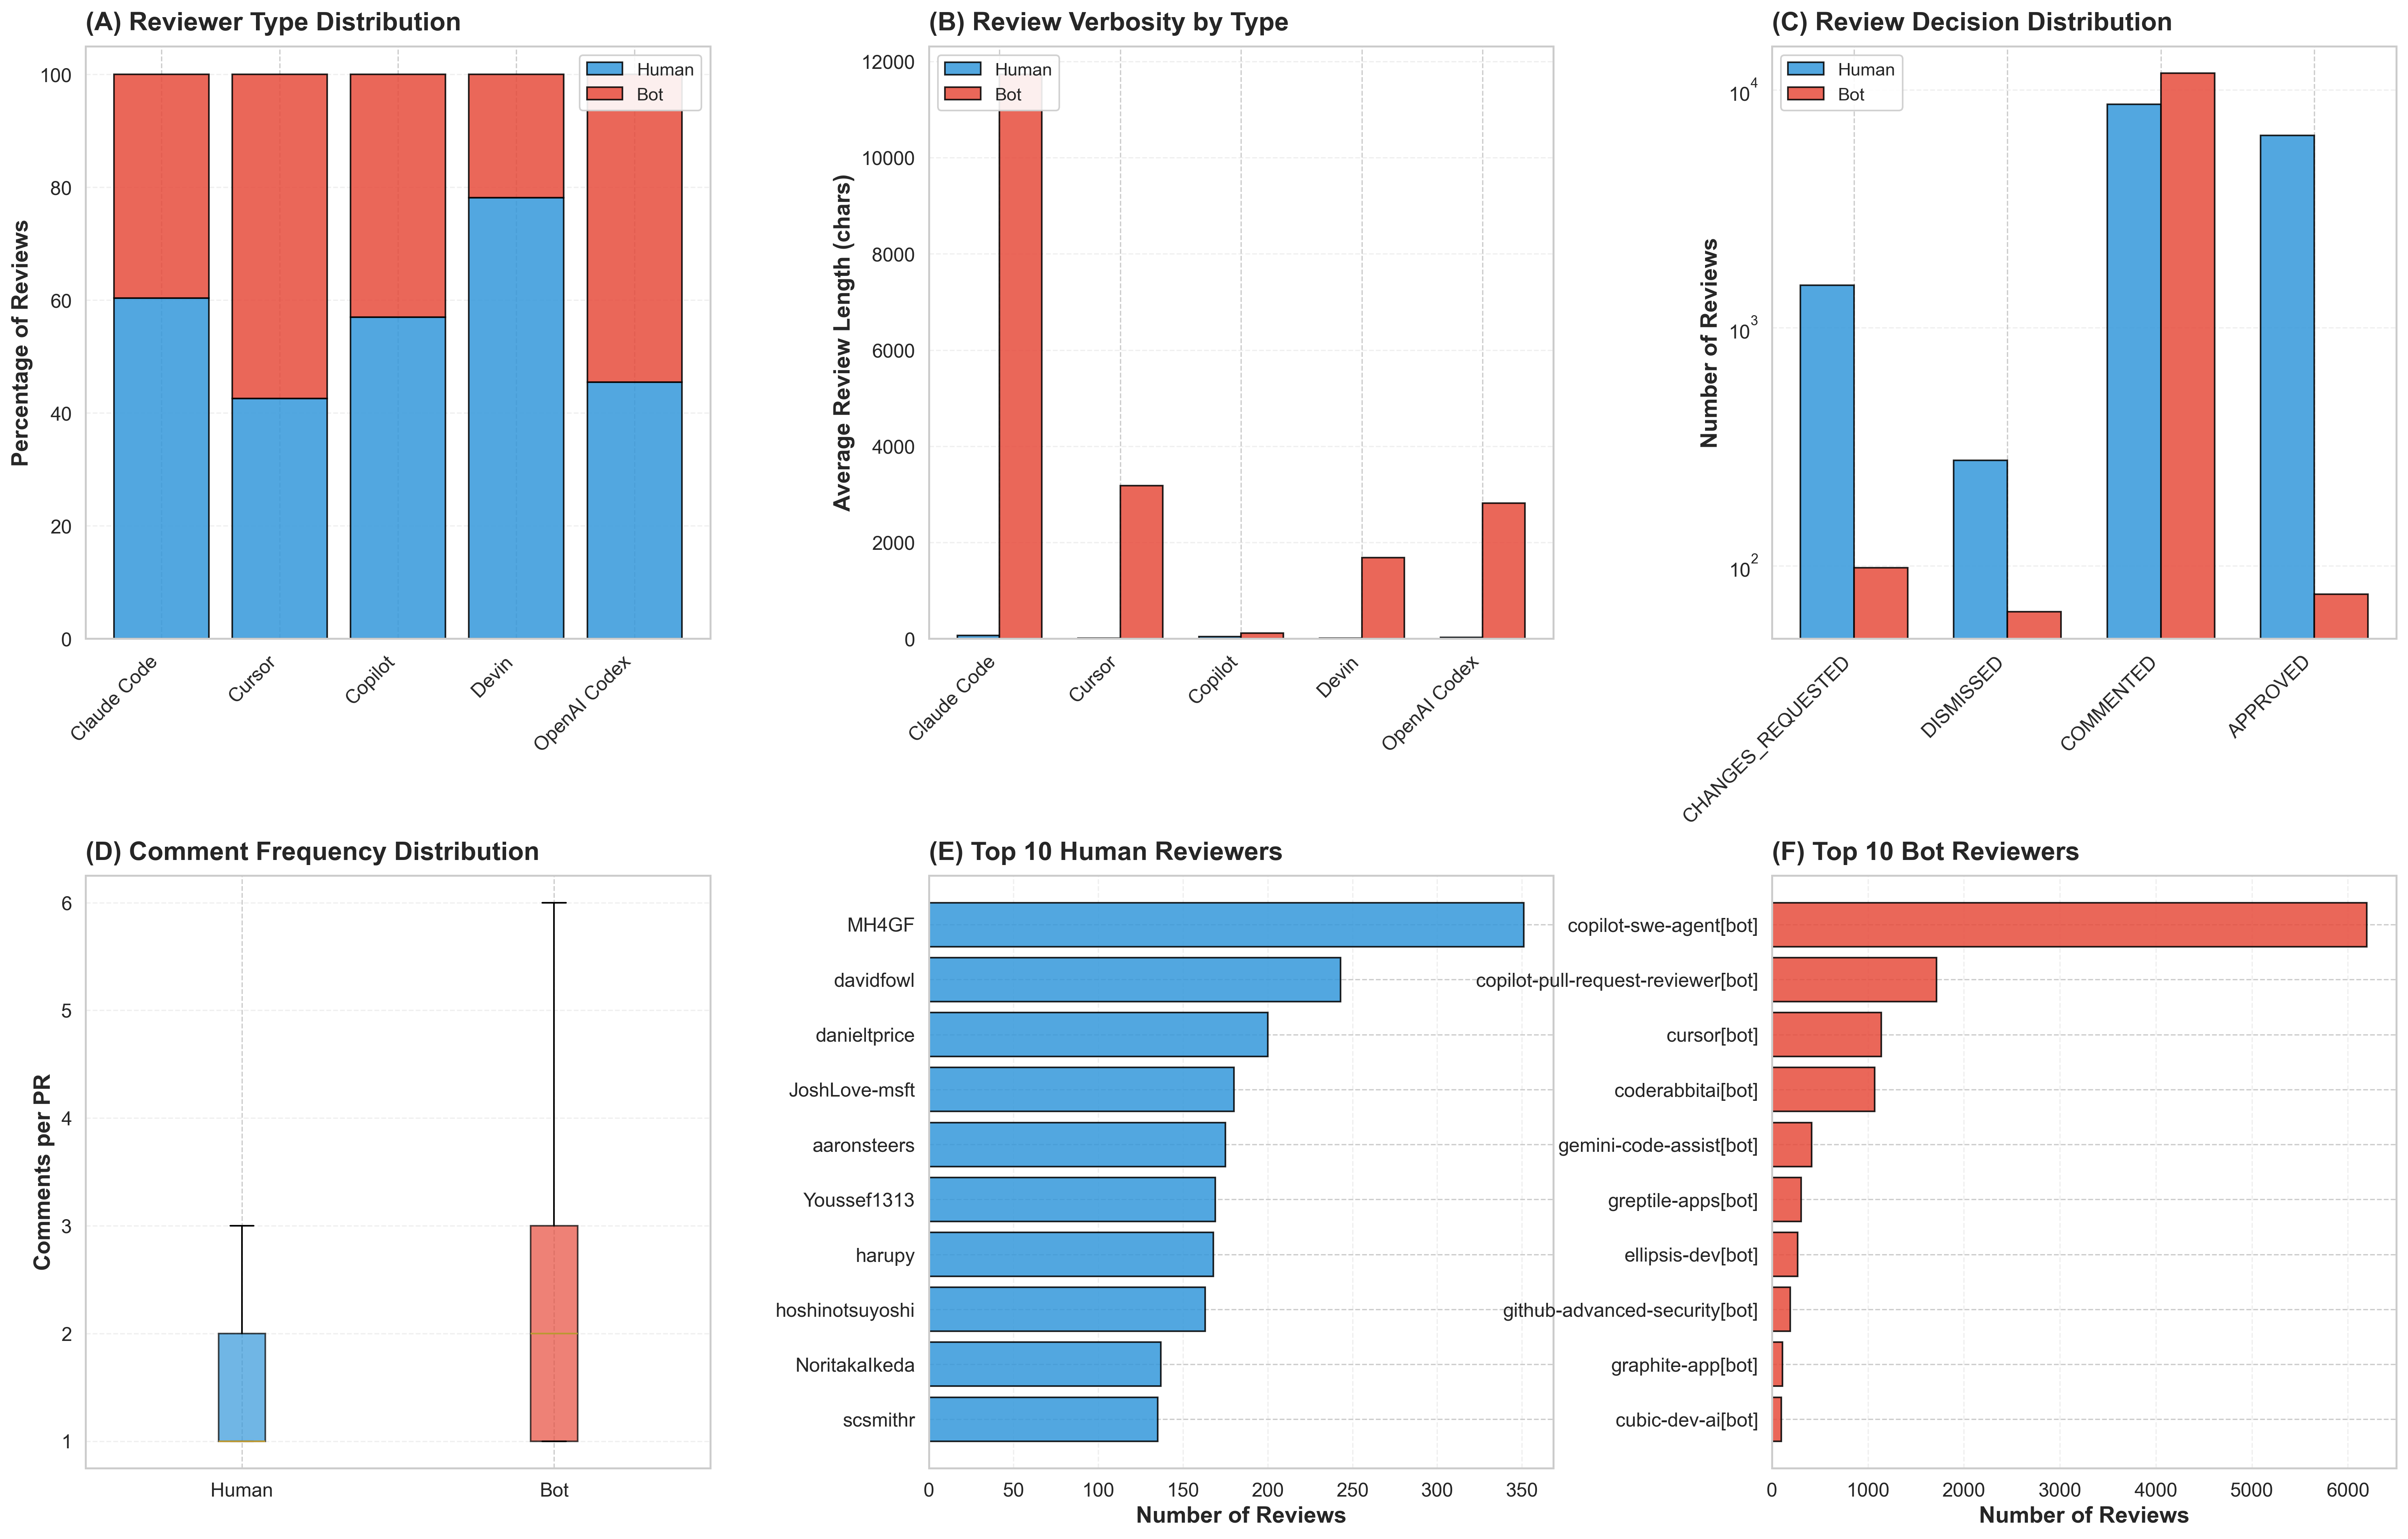
\includegraphics[width=\textwidth]{figures/fig5_human_vs_bot_engagement.png}
\caption{Human vs Bot Reviewer Engagement: Six-panel analysis showing reviewer type distribution (58.5\% human, 41.5\% bot), review verbosity comparison, review decisions, comment frequency, and top reviewers. Bots write longer reviews (avg 11,700 chars) vs humans (avg 200 chars).}
\label{fig:human_bot}
\end{figure}

\newpage
\section*{Appendix: Comprehensive Statistical Summary}

This appendix provides detailed statistical measures for all key entities, including higher-order moments (skewness, kurtosis) that reveal the distribution characteristics.

\begin{table}[H]
\centering
\caption{Comprehensive Entity Statistics (Part 1: PR and File Metrics)}
\tiny
\begin{tabular}{@{}lrrrrrrrrrrr@{}}
\toprule
\textbf{Entity} & \textbf{Count} & \textbf{Mean} & \textbf{Median} & \textbf{Std Dev} & \textbf{Min} & \textbf{25\%} & \textbf{75\%} & \textbf{Max} & \textbf{IQR} & \textbf{Skew} & \textbf{Kurt} \\
\midrule
PR Title Length (chars) & 33,596 & 42.85 & 39.0 & 18.13 & 1.0 & 30.0 & 51.0 & 351 & 21.0 & 2.00 & 13.03 \\
PR Body Length (chars) & 33,596 & 930.84 & 383.0 & 1,651.27 & 0.0 & 273.0 & 935.3 & 77,435 & 662.3 & 13.03 & 347.55 \\
PR Body Lines & 33,596 & 21.59 & 11.0 & 31.15 & 1.0 & 9.0 & 20.0 & 2,076 & 11.0 & 15.58 & 719.32 \\
Lines Added per File & 524,457 & 49.84 & 4.0 & 688.10 & 0.0 & 1.0 & 22.0 & 170,444 & 21.0 & 112.83 & 19,769.64 \\
Lines Deleted per File & 524,457 & 24.04 & 1.0 & 542.81 & 0.0 & 0.0 & 4.0 & 105,024 & 4.0 & 88.39 & 10,850.88 \\
Total Changes per File & 524,457 & 73.88 & 8.0 & 945.68 & 0.0 & 2.0 & 34.0 & 171,263 & 32.0 & 69.23 & 7,298.63 \\
Total Lines Added per PR & 33,580 & 778.37 & 46.0 & 6,351.43 & 0.0 & 5.0 & 175.0 & 631,203 & 170.0 & 43.56 & 3,366.62 \\
Total Lines Deleted per PR & 33,580 & 375.52 & 5.0 & 4,835.82 & 0.0 & 0.0 & 38.0 & 640,627 & 38.0 & 81.33 & 9,729.96 \\
Files Changed per PR & 33,580 & 15.62 & 3.0 & 54.67 & 0.0 & 1.0 & 8.0 & 2,682 & 7.0 & 11.96 & 302.12 \\
\bottomrule
\end{tabular}
\end{table}

\begin{table}[H]
\centering
\caption{Comprehensive Entity Statistics (Part 2: Comments, Reviews, and User Metrics)}
\tiny
\begin{tabular}{@{}lrrrrrrrrrrr@{}}
\toprule
\textbf{Entity} & \textbf{Count} & \textbf{Mean} & \textbf{Median} & \textbf{Std Dev} & \textbf{Min} & \textbf{25\%} & \textbf{75\%} & \textbf{Max} & \textbf{IQR} & \textbf{Skew} & \textbf{Kurt} \\
\midrule
Comment Length (chars) & 39,122 & 1,604.62 & 404.0 & 5,607.40 & 1.0 & 154.0 & 1,248.0 & 223,759 & 1,094.0 & 16.61 & 390.22 \\
Review Length (chars) & 28,875 & 584.30 & 0.0 & 3,471.45 & 0.0 & 0.0 & 9.0 & 155,434 & 9.0 & 22.25 & 703.87 \\
User Followers & 1,796 & 372.18 & 58.0 & 1,916.52 & 0.0 & 14.0 & 195.0 & 45,077 & 181.0 & 15.25 & 287.35 \\
User Following & 1,796 & 50.45 & 10.0 & 235.72 & 0.0 & 2.0 & 39.3 & 8,049 & 37.3 & 24.66 & 773.64 \\
Repository Stars & 2,807 & 4,273.75 & 564.0 & 12,634.83 & 101.0 & 215.5 & 2,487.5 & 203,424 & 2,272.0 & 7.08 & 70.14 \\
Repository Forks & 2,807 & 750.35 & 104.0 & 3,135.61 & 1.0 & 36.0 & 399.5 & 62,633 & 363.5 & 12.10 & 181.13 \\
\bottomrule
\end{tabular}
\end{table}

\textbf{Interpretation Notes:}
\begin{itemize}
    \item \textbf{High Skewness (>2)}: All metrics show strong right-skewed distributions, indicating most values are small with occasional extreme outliers
    \item \textbf{Extreme Kurtosis}: Values ranging from 13 to 19,770 indicate heavy-tailed distributions with extreme outliers
    \item \textbf{Large Mean-Median Gap}: Confirms outlier influence (e.g., mean files/PR: 15.62 vs median: 3.0)
    \item \textbf{IQR Analysis}: Interquartile ranges are small relative to maximums, showing most data is concentrated in lower ranges
\end{itemize}

\end{document}